\section{Non signal testing of the regular and variational Autoencoder}\label{sec:nonsig}

\subsection*{Channel removing}

Both the large and small regular and variational autoencoder produced results, and the results are shown below. 
The Higgs, singletop and ttbar channels have been selected here, as they are 
from a physics standpoint the channels that looks most unlike the other channels.  


\begin{figure}[H]
    \centering
    \begin{subfigure}{.45\textwidth}
        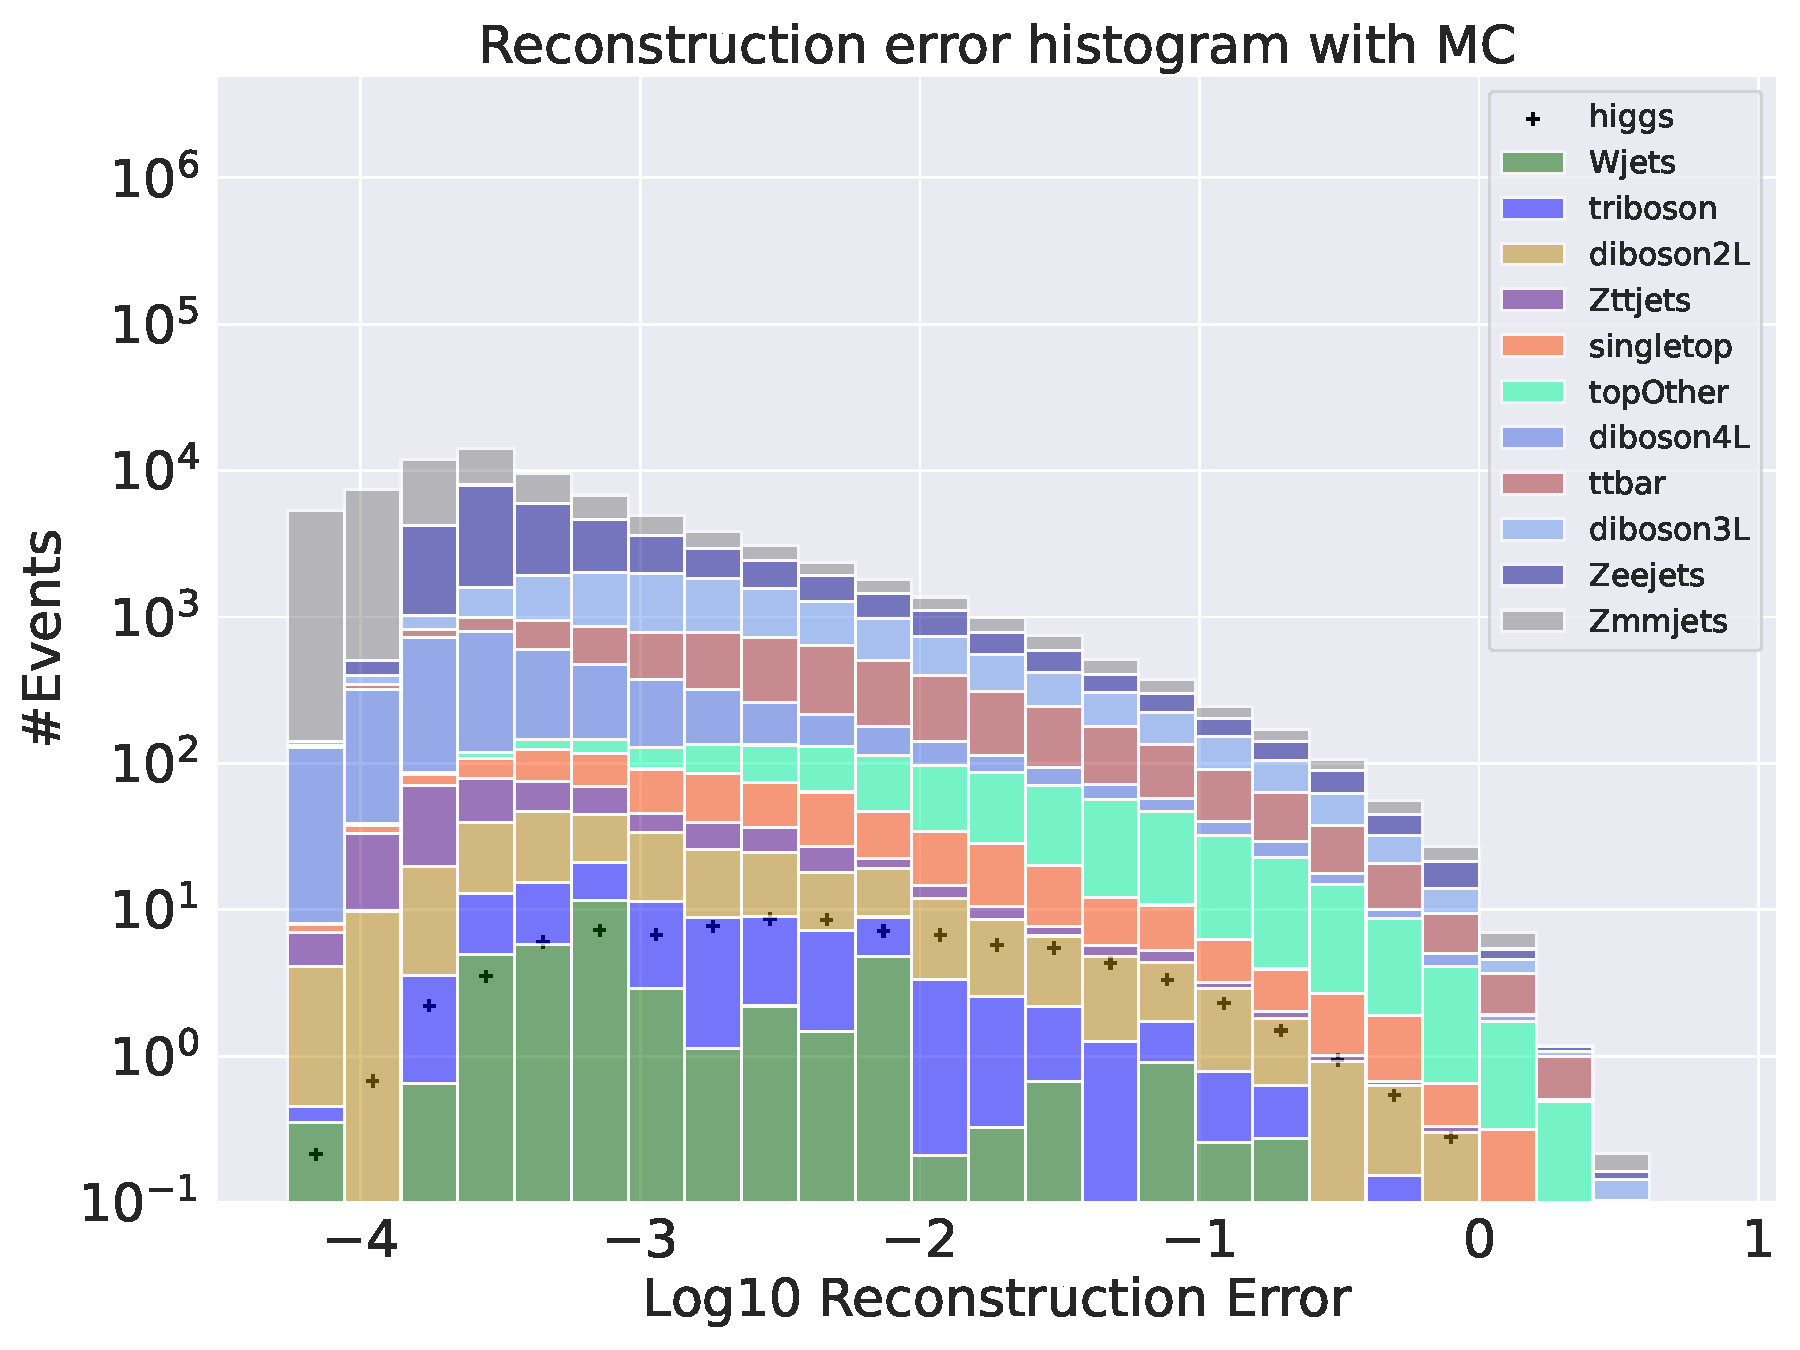
\includegraphics[width=\textwidth]{Figures/AE_testing/small/b_data_recon_big_rm3_feats_sig_higgs.pdf}
        \caption{}
        \label{fig:ae_small_higgs}
    \end{subfigure}
    \hfill 
    \begin{subfigure}{.45\textwidth}
        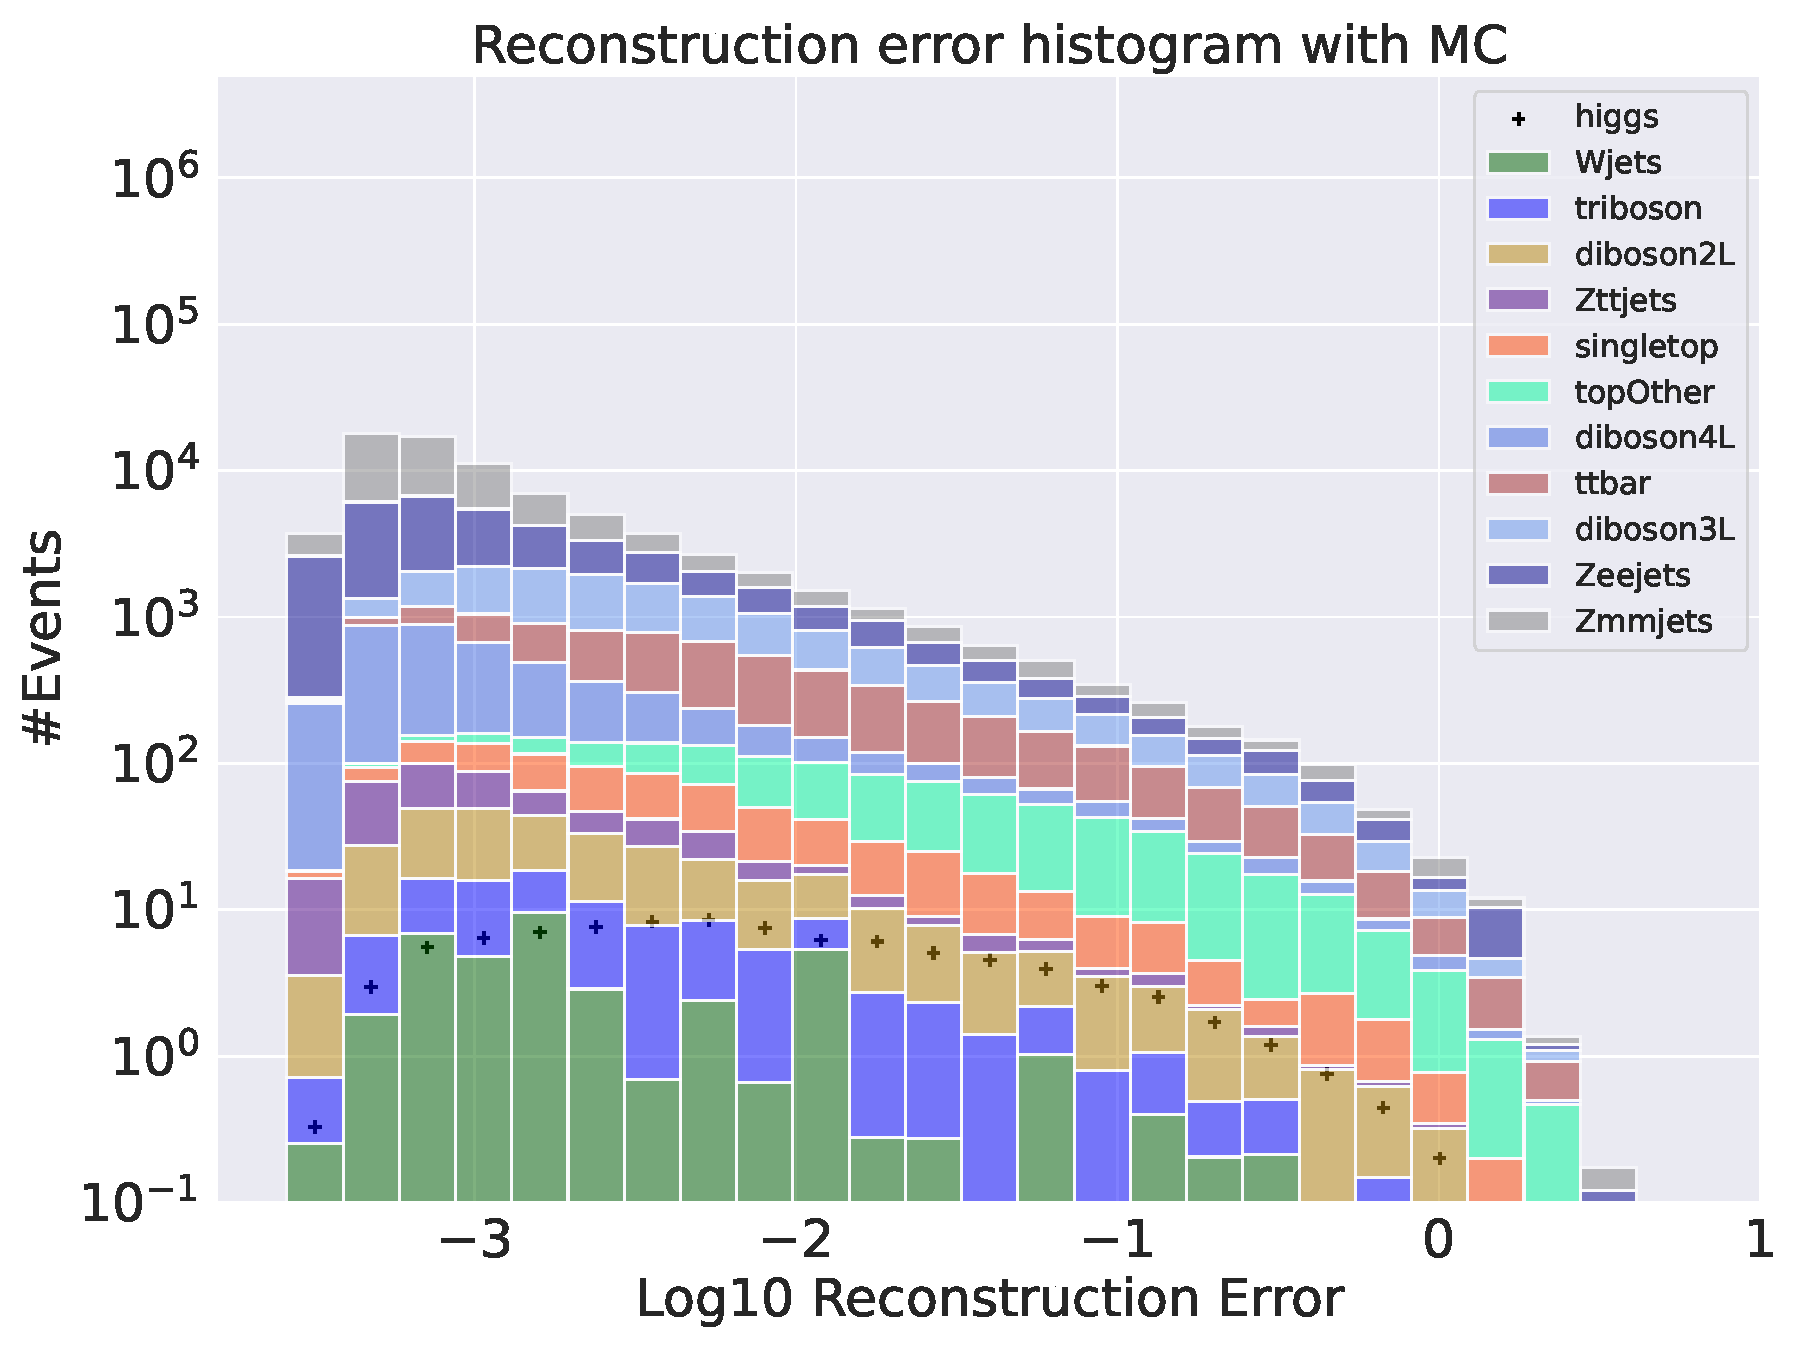
\includegraphics[width=\textwidth]{Figures/AE_testing/big/b_data_recon_big_rm3_feats_sig_higgs.pdf}
        \caption{ }
        \label{fig:ae_big_higgs}
    \end{subfigure}
    \hfill 
    \caption[AE | Reconstruction error using Higgs channel as signal]{Reconstruction error on validation SM MC from the small (a) and large (b) Autoencoders. The higgs channel has been removed from training and 
    is used as signal. No significant difference in distributions is found.  } 
    \label{fig:ae_big_channel_1}
    
\end{figure}

\begin{figure}[H]
    \centering
    \begin{subfigure}{.45\textwidth}
        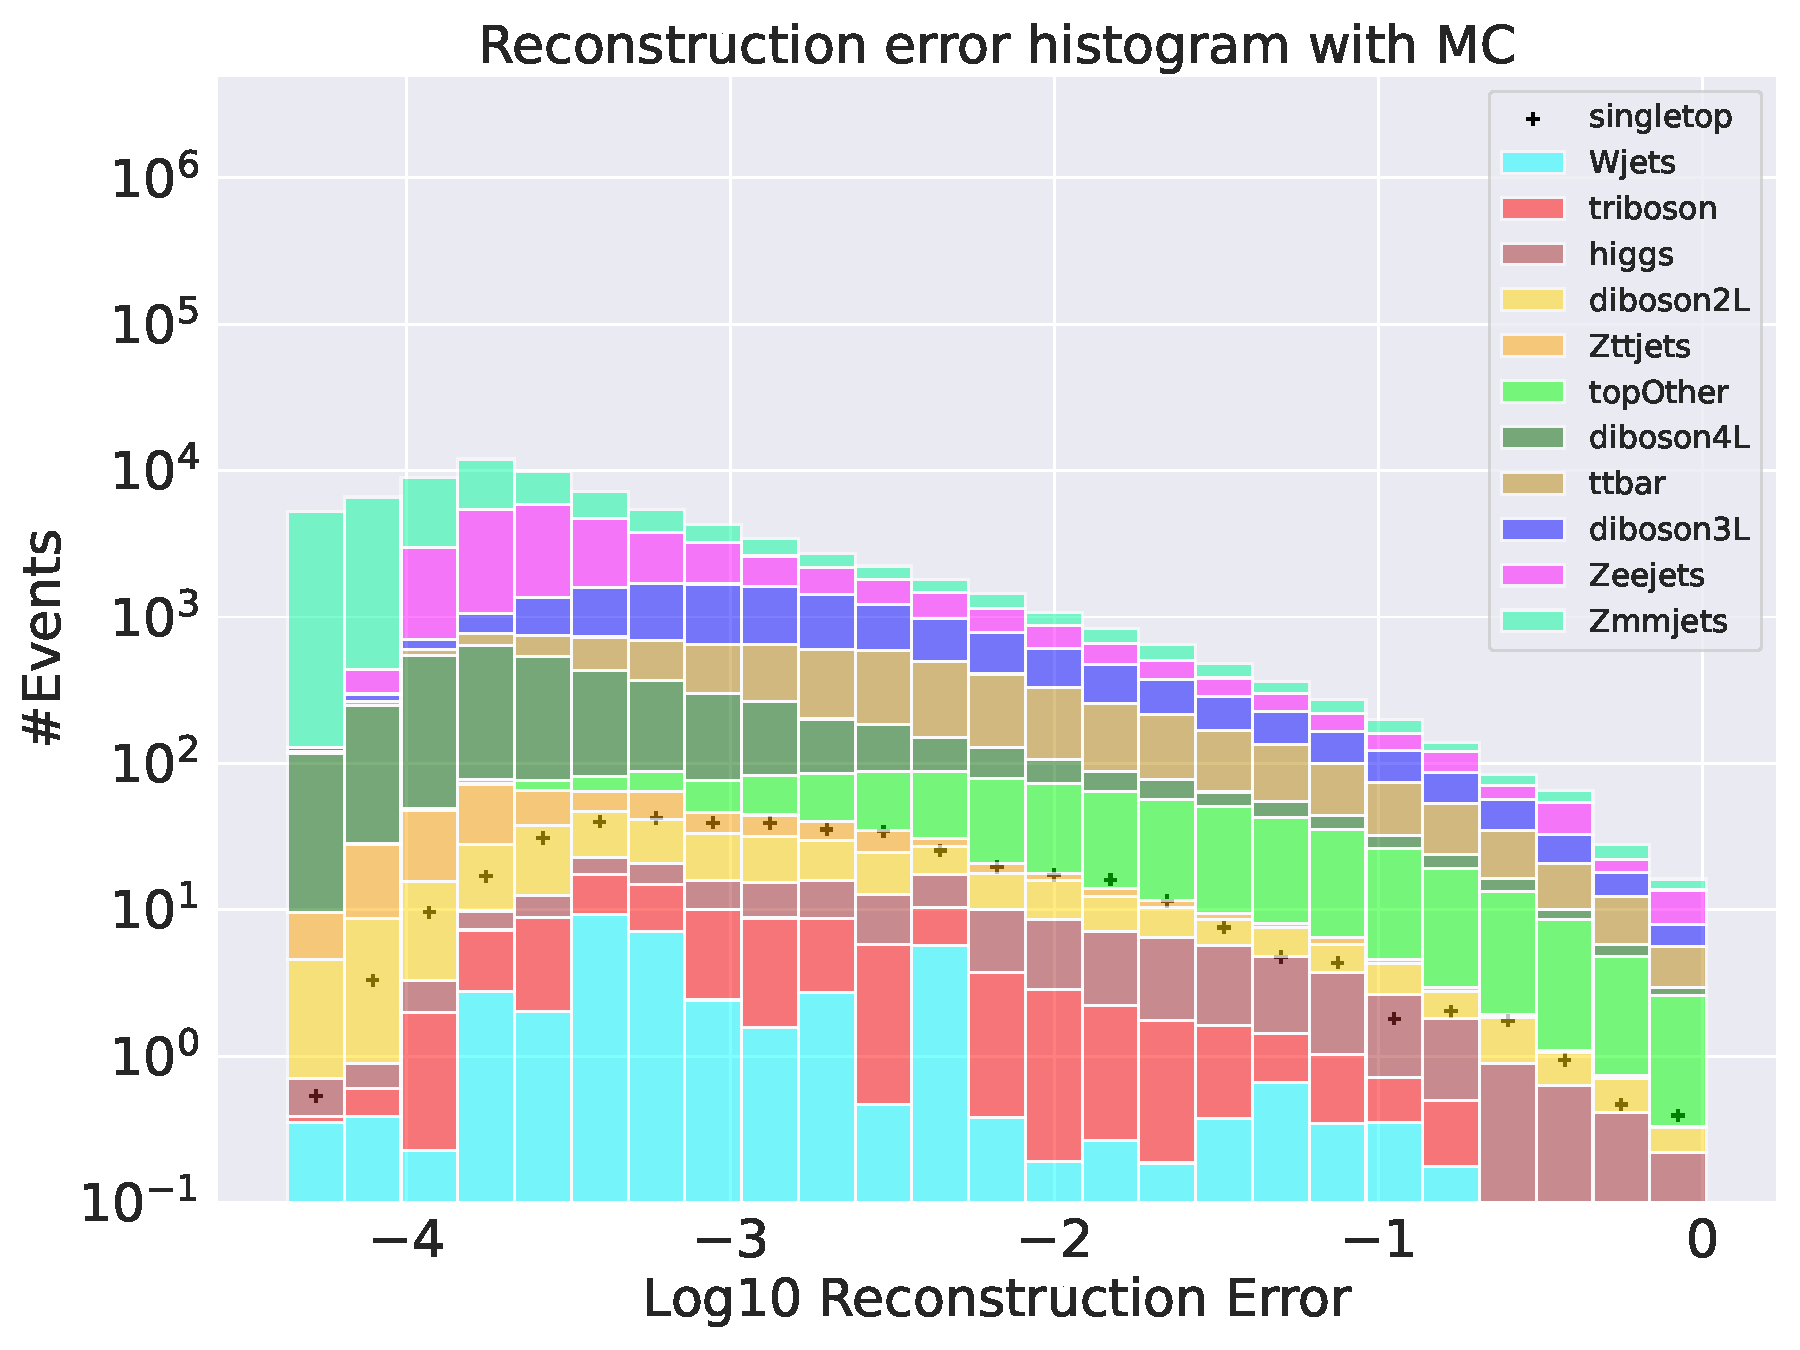
\includegraphics[width=\textwidth]{Figures/AE_testing/small/b_data_recon_big_rm3_feats_sig_singletop.pdf}
        \caption{}
        \label{fig:ae_small_singletop}
    \end{subfigure}
    \hfill
    \begin{subfigure}{.45\textwidth}
        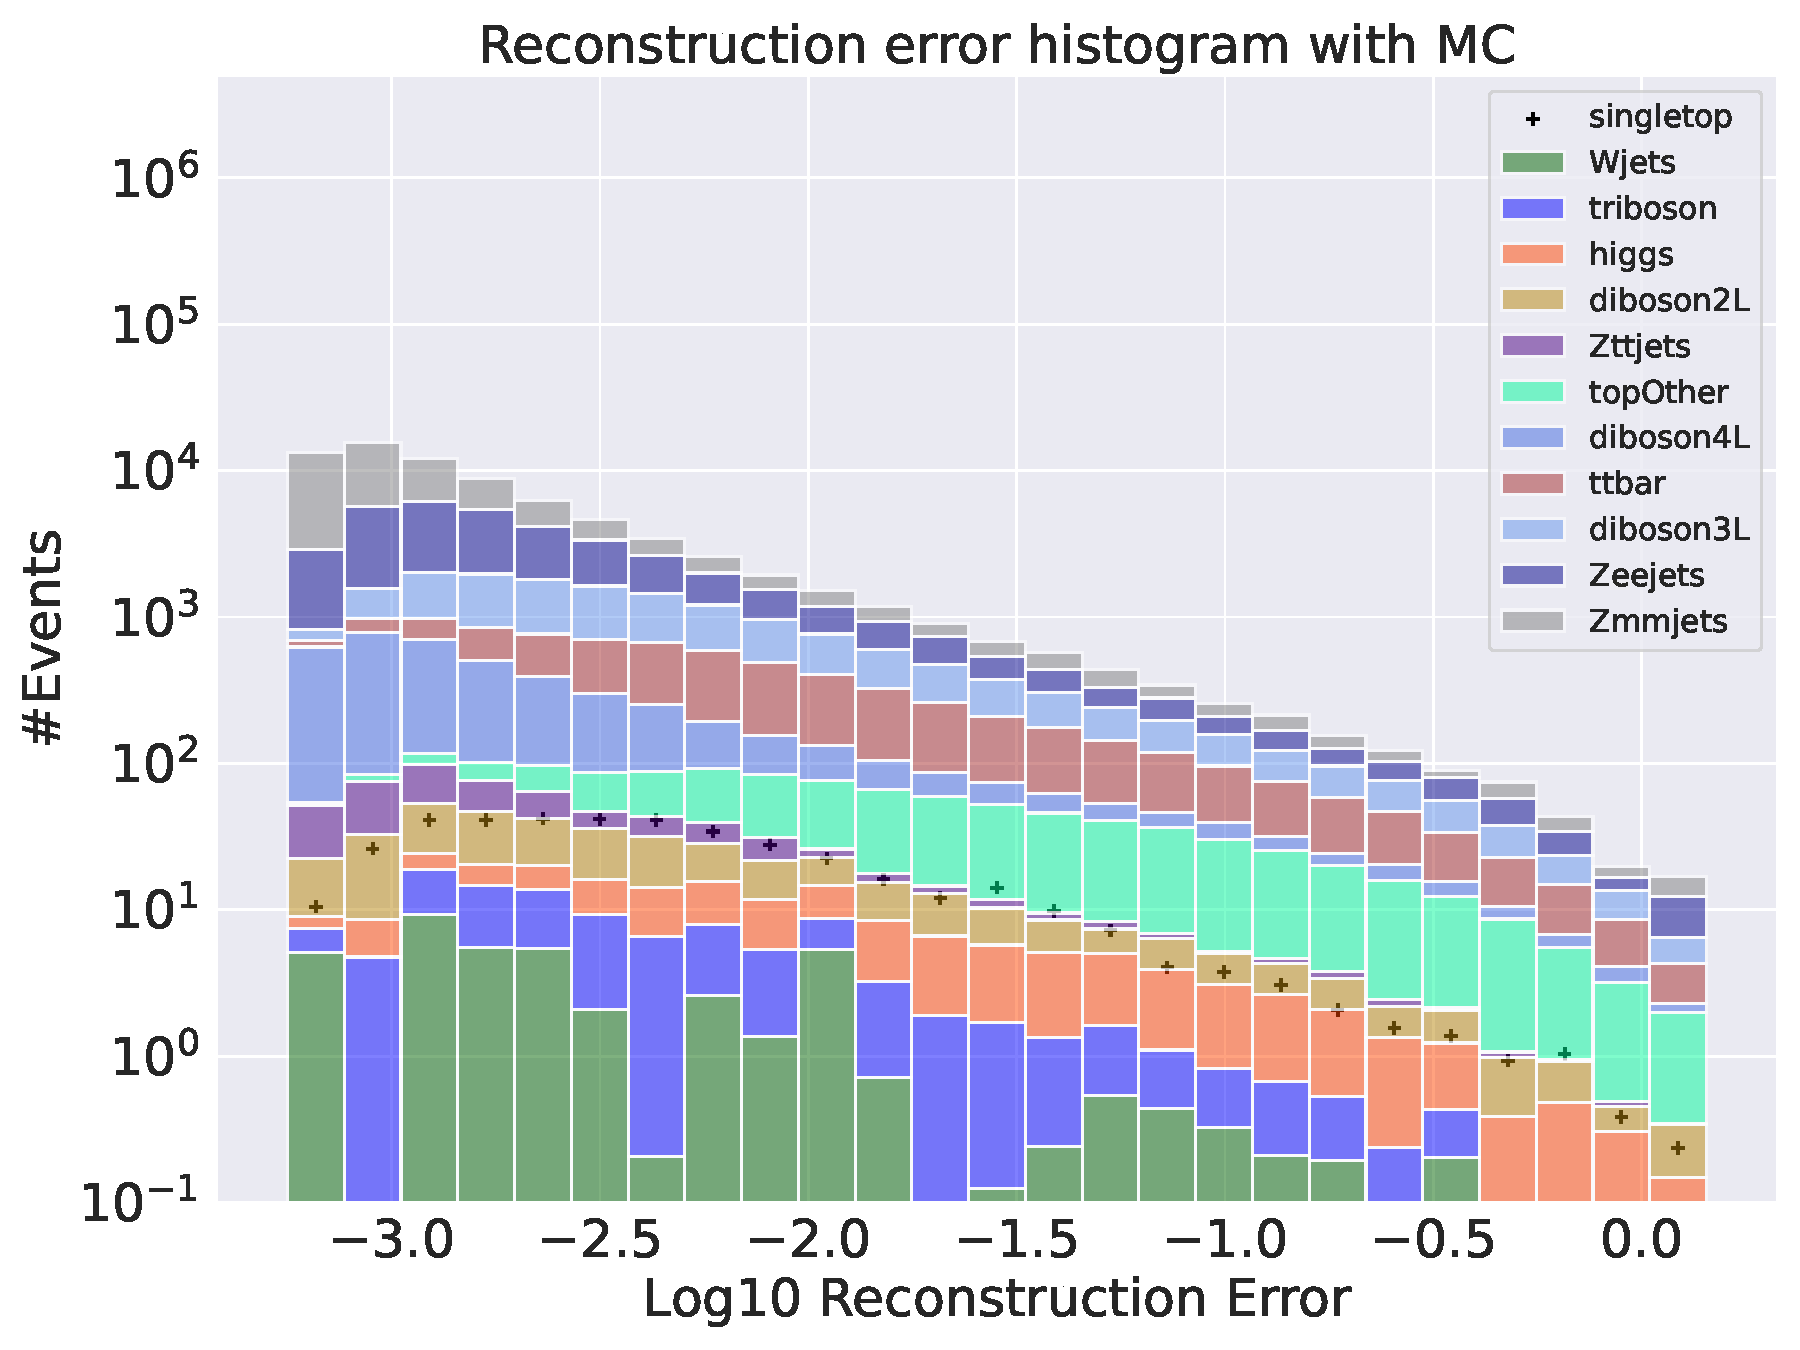
\includegraphics[width=\textwidth]{Figures/AE_testing/big/b_data_recon_big_rm3_feats_sig_singletop.pdf}
        \caption{ }
        \label{fig:ae_big_singletop}
    \end{subfigure}
    \hfill
    \caption[AE | Reconstruction error using Singletop channel as signal]{Reconstruction error on validation SM MC from the small (a) and large (b) Autoencoders. The singletop channel has been removed from training and 
    is used as signal. No significant difference in distributions is found.  } 
    \label{fig:ae_big_channel_2}
\end{figure}

\begin{figure}[H]
    \centering
    \begin{subfigure}{.45\textwidth}
        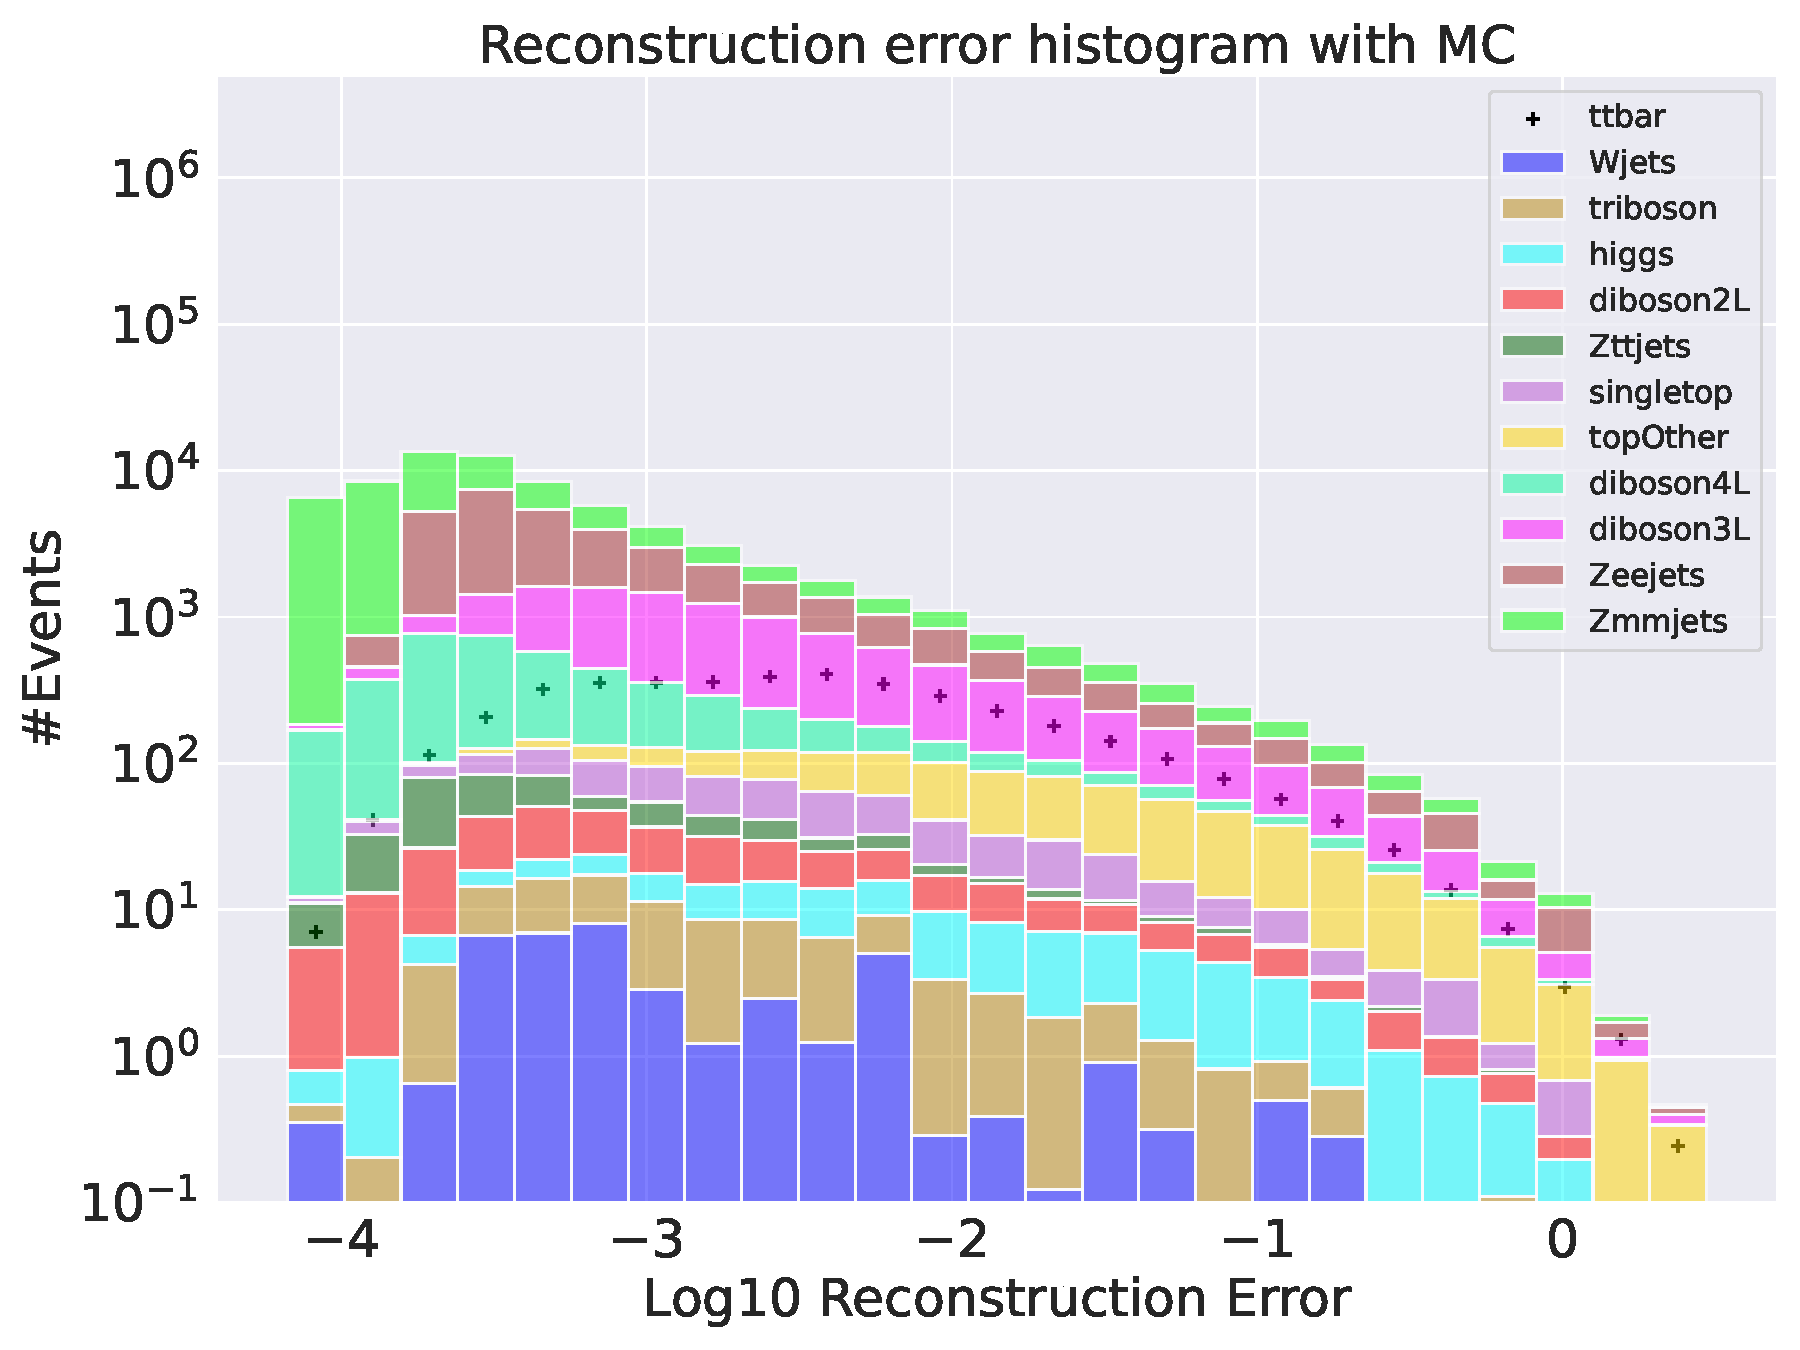
\includegraphics[width=\textwidth]{Figures/AE_testing/small/b_data_recon_big_rm3_feats_sig_ttbar.pdf}
        \caption{}
        \label{fig:ae_small_ttbar}
    \end{subfigure}
    \hfill 
    \begin{subfigure}{.45\textwidth}
        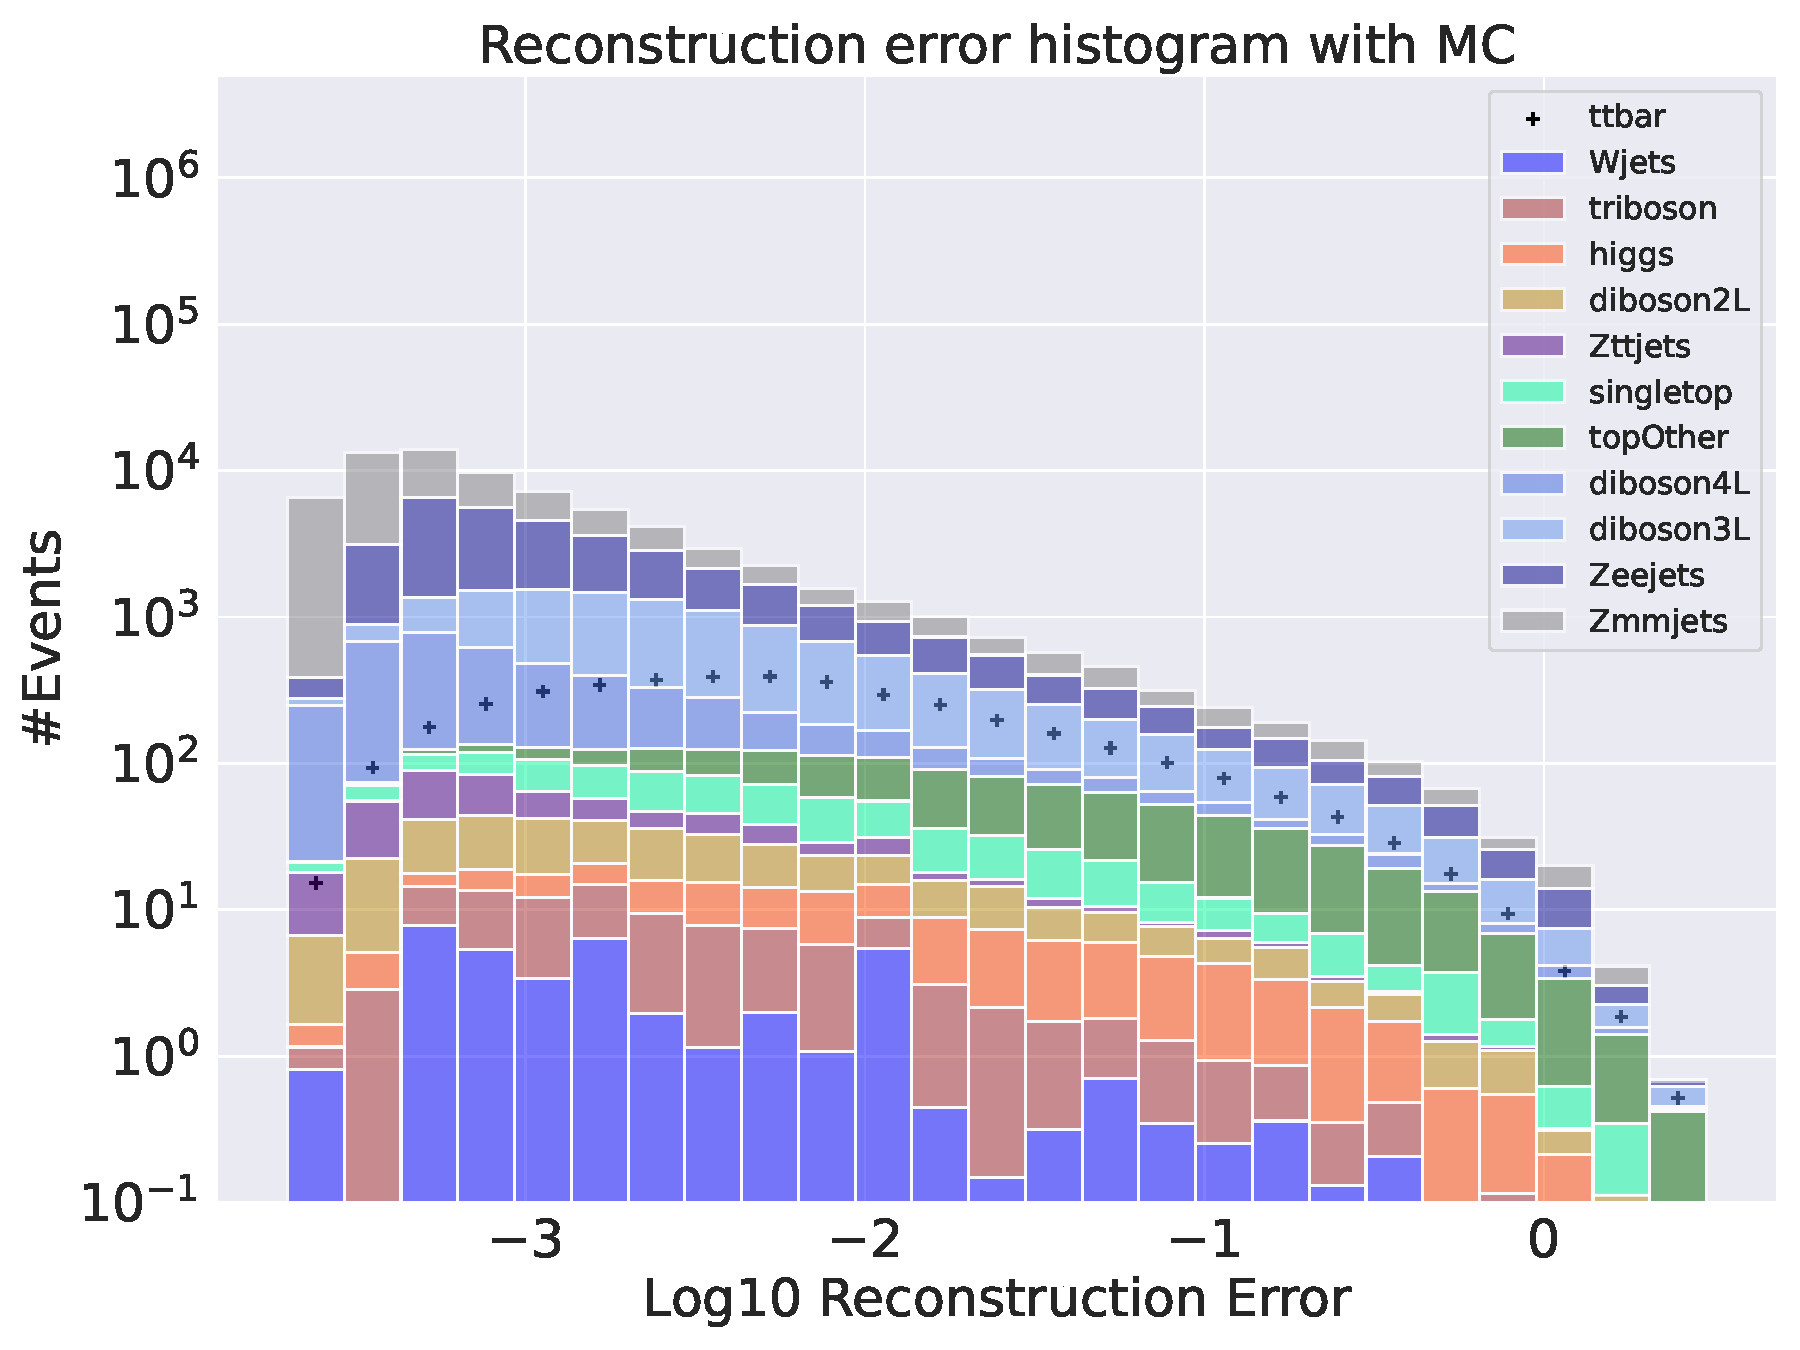
\includegraphics[width=\textwidth]{Figures/AE_testing/big/b_data_recon_big_rm3_feats_sig_ttbar.pdf}
        \caption{ }
        \label{fig:ae_big_ttbar}
    \end{subfigure}
    \hfill 
    \caption[AE | Reconstruction error using ttbar channel as signal]{Reconstruction error on validation SM MC from the small (a) and large (b) Autoencoder. The ttbar channel has been removed from training and 
    is used as signal. No significant difference in distributions is found.  }
    \label{fig:ae_big_channel_3}
\end{figure}



\begin{figure}[H]
    \centering
    \begin{subfigure}{.45\textwidth}
        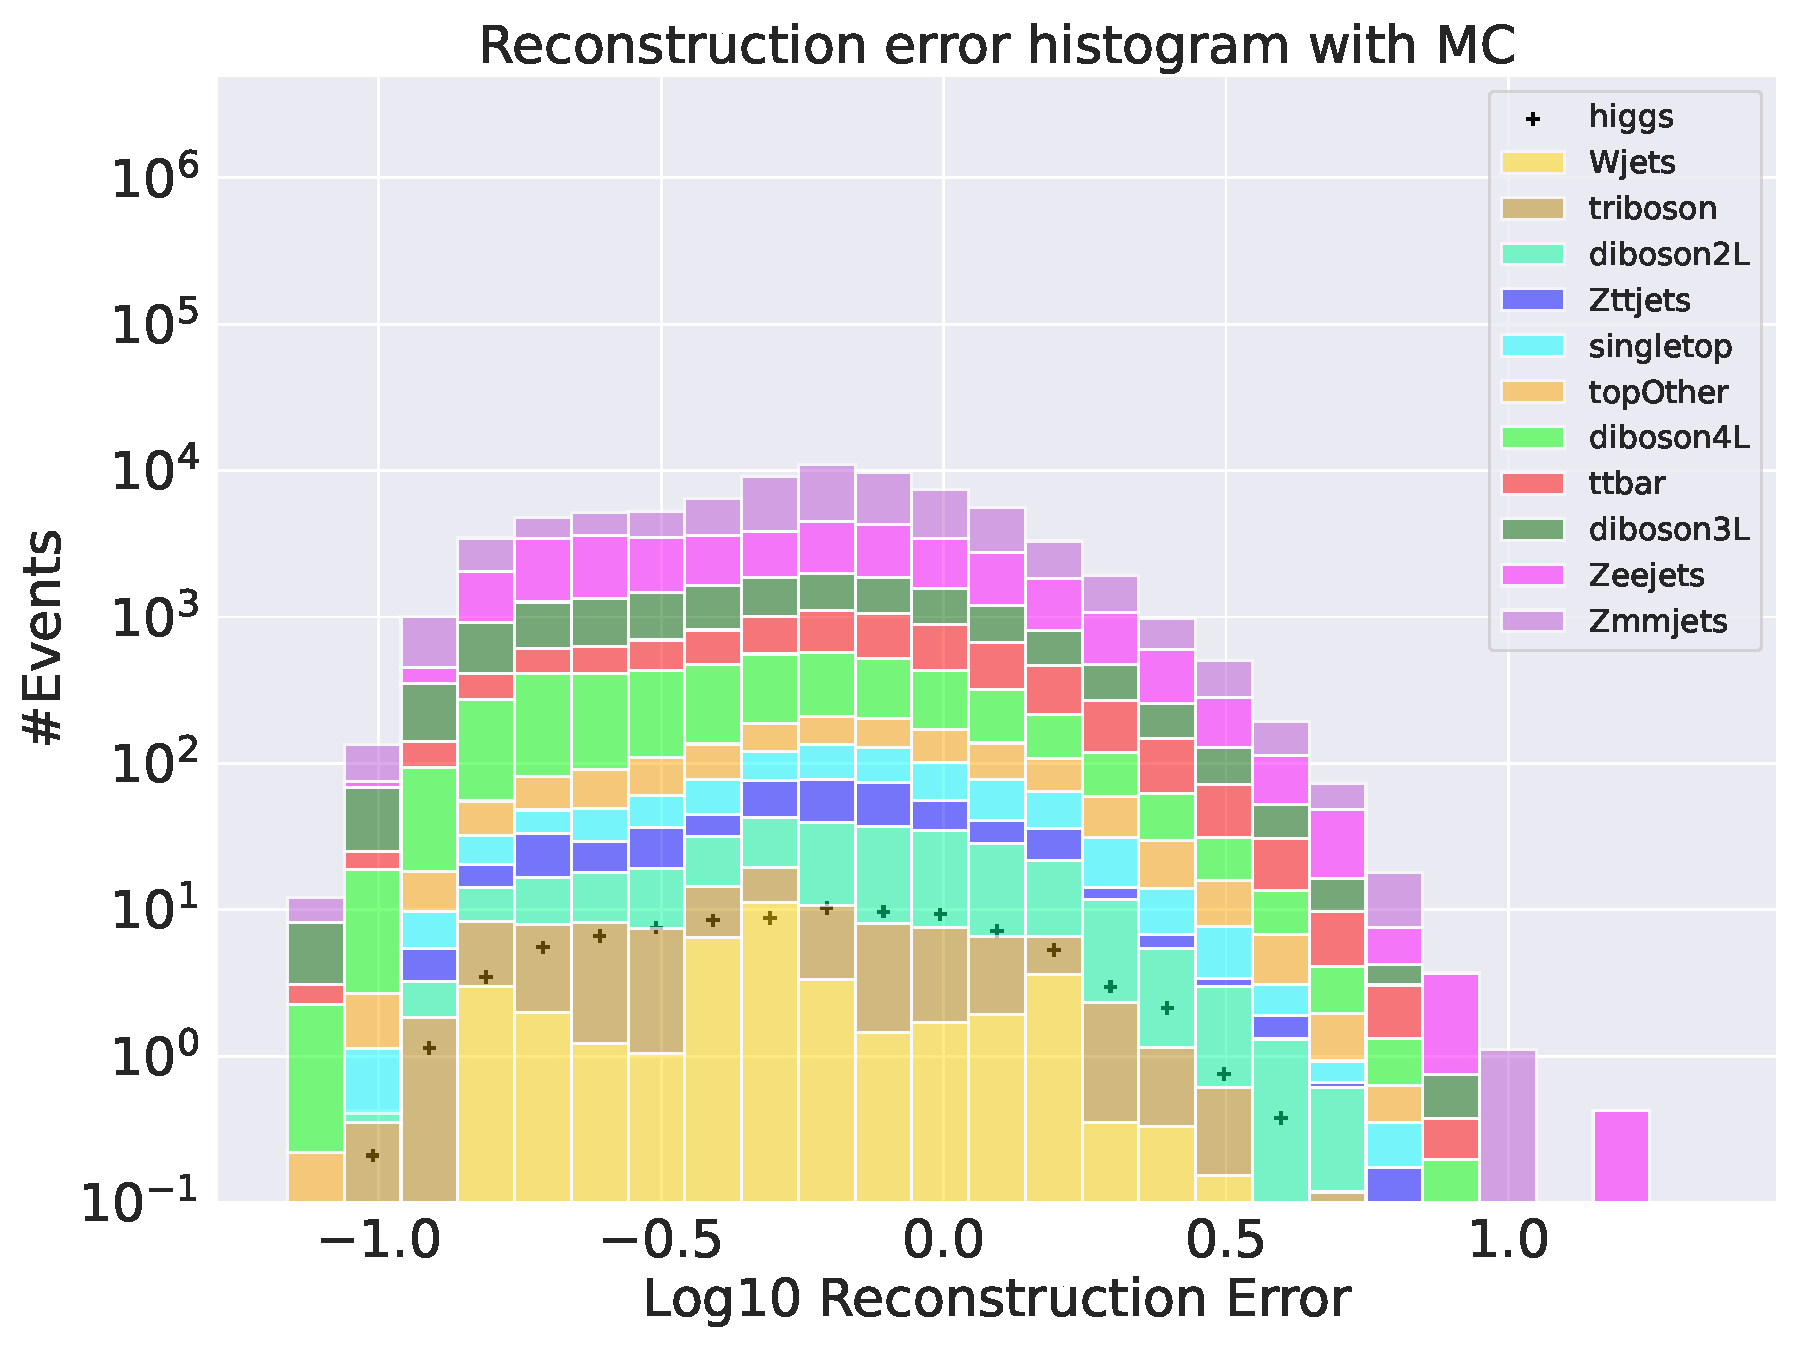
\includegraphics[width=\textwidth]{Figures/VAE_testing/small/b_data_recon_big_rm3_feats_sig_higgs.pdf}
        \caption{}
        \label{fig:vae_small_higgs}
    \end{subfigure}
    \hfill 
    \begin{subfigure}{.45\textwidth}
        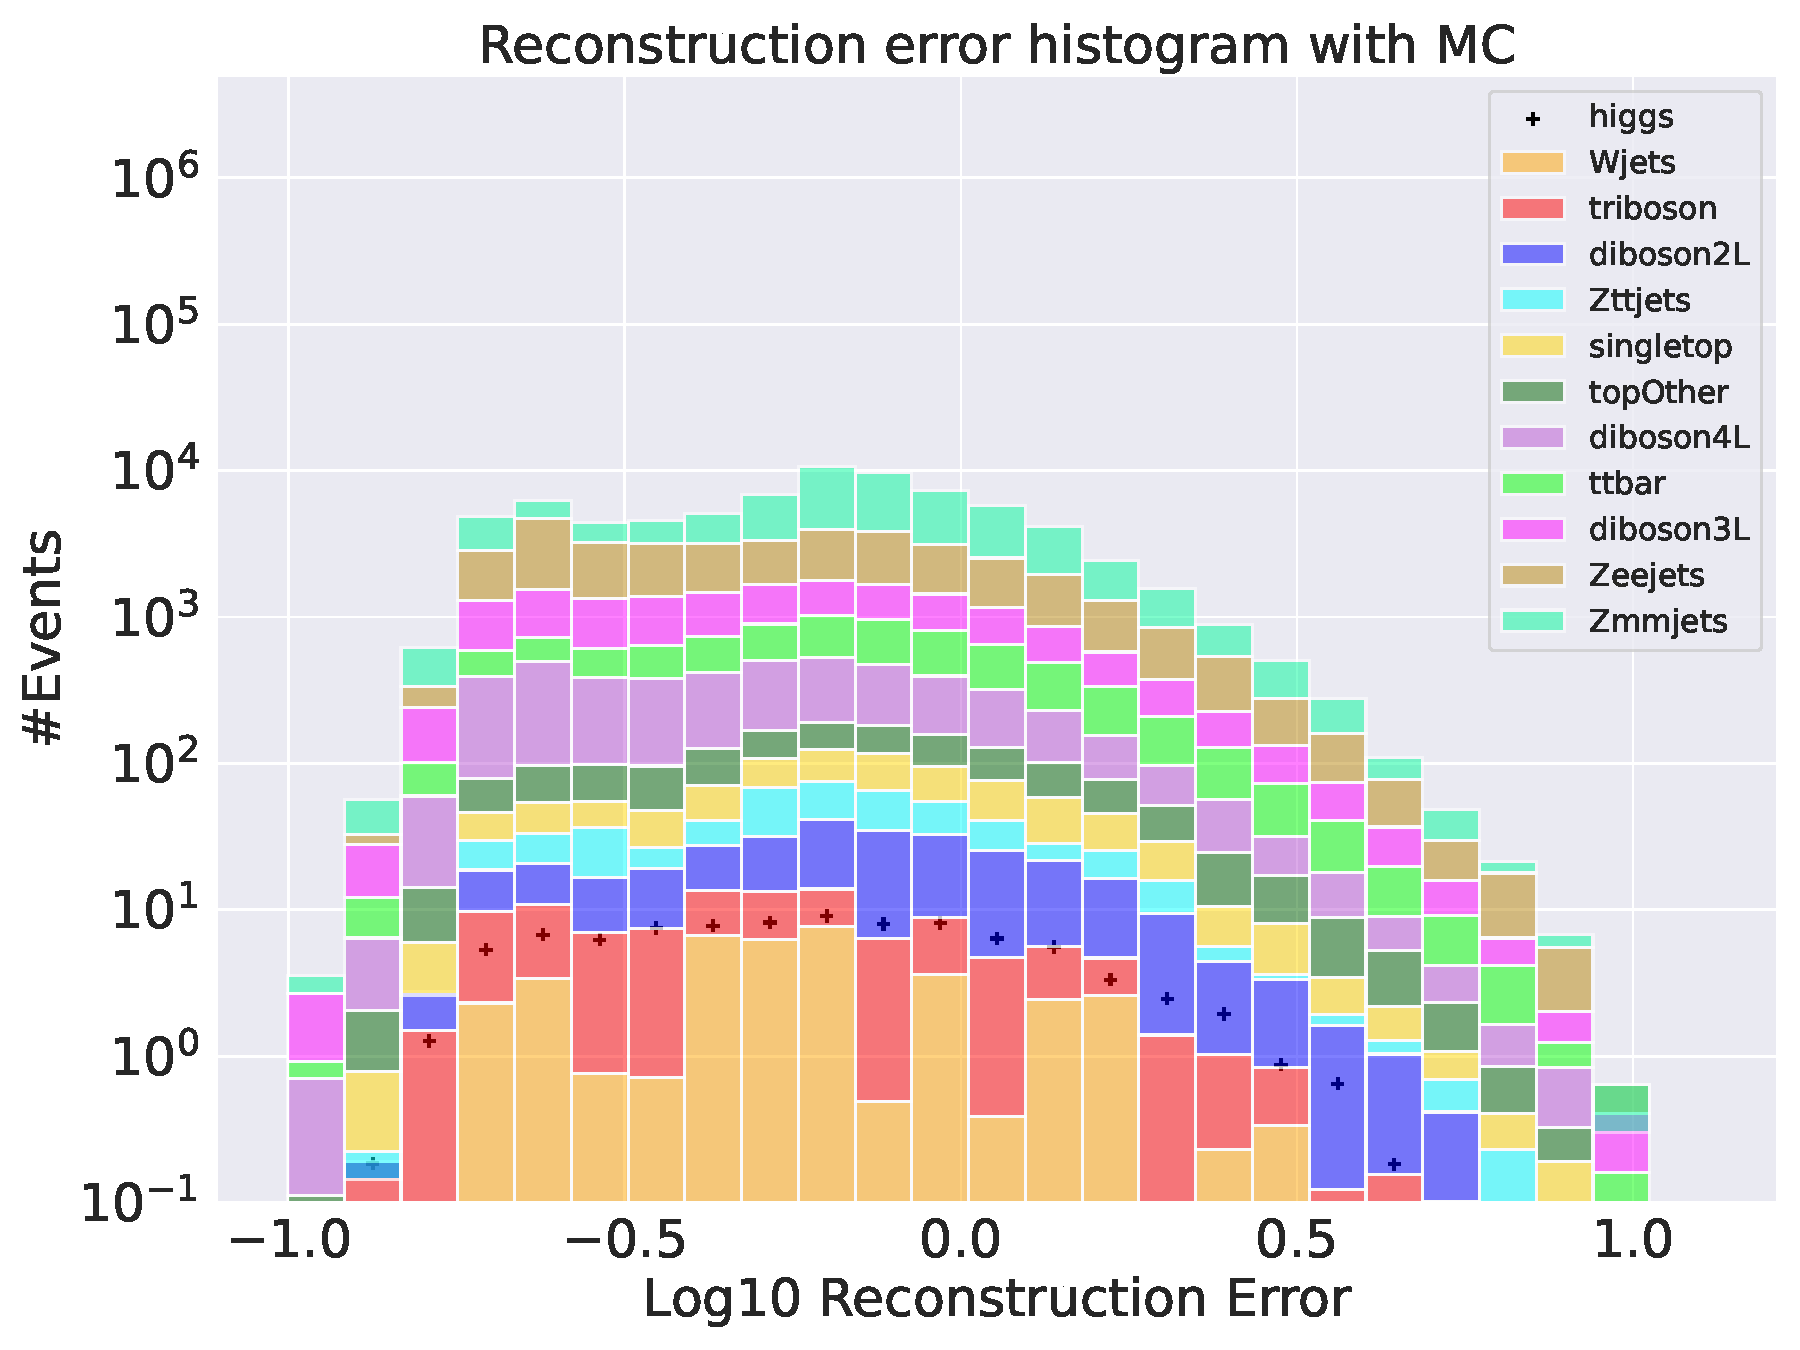
\includegraphics[width=\textwidth]{Figures/VAE_testing/big/b_data_recon_big_rm3_feats_sig_higgs.pdf}
        \caption{ }
        \label{fig:vae_big_higgs}
    \end{subfigure}
    \hfill  
    \caption[VAE | Reconstruction error using Higgs channel as signal]{Reconstruction error on validation SM MC from the small (a) and large (b) variational Autoencoder. The higgs channel has been removed from training and 
    is used as signal. No significant difference in distributions is found. }
    \label{fig:vae_big_channel_1}
\end{figure}

\begin{figure}[H]
    \centering
    \begin{subfigure}{.45\textwidth}
        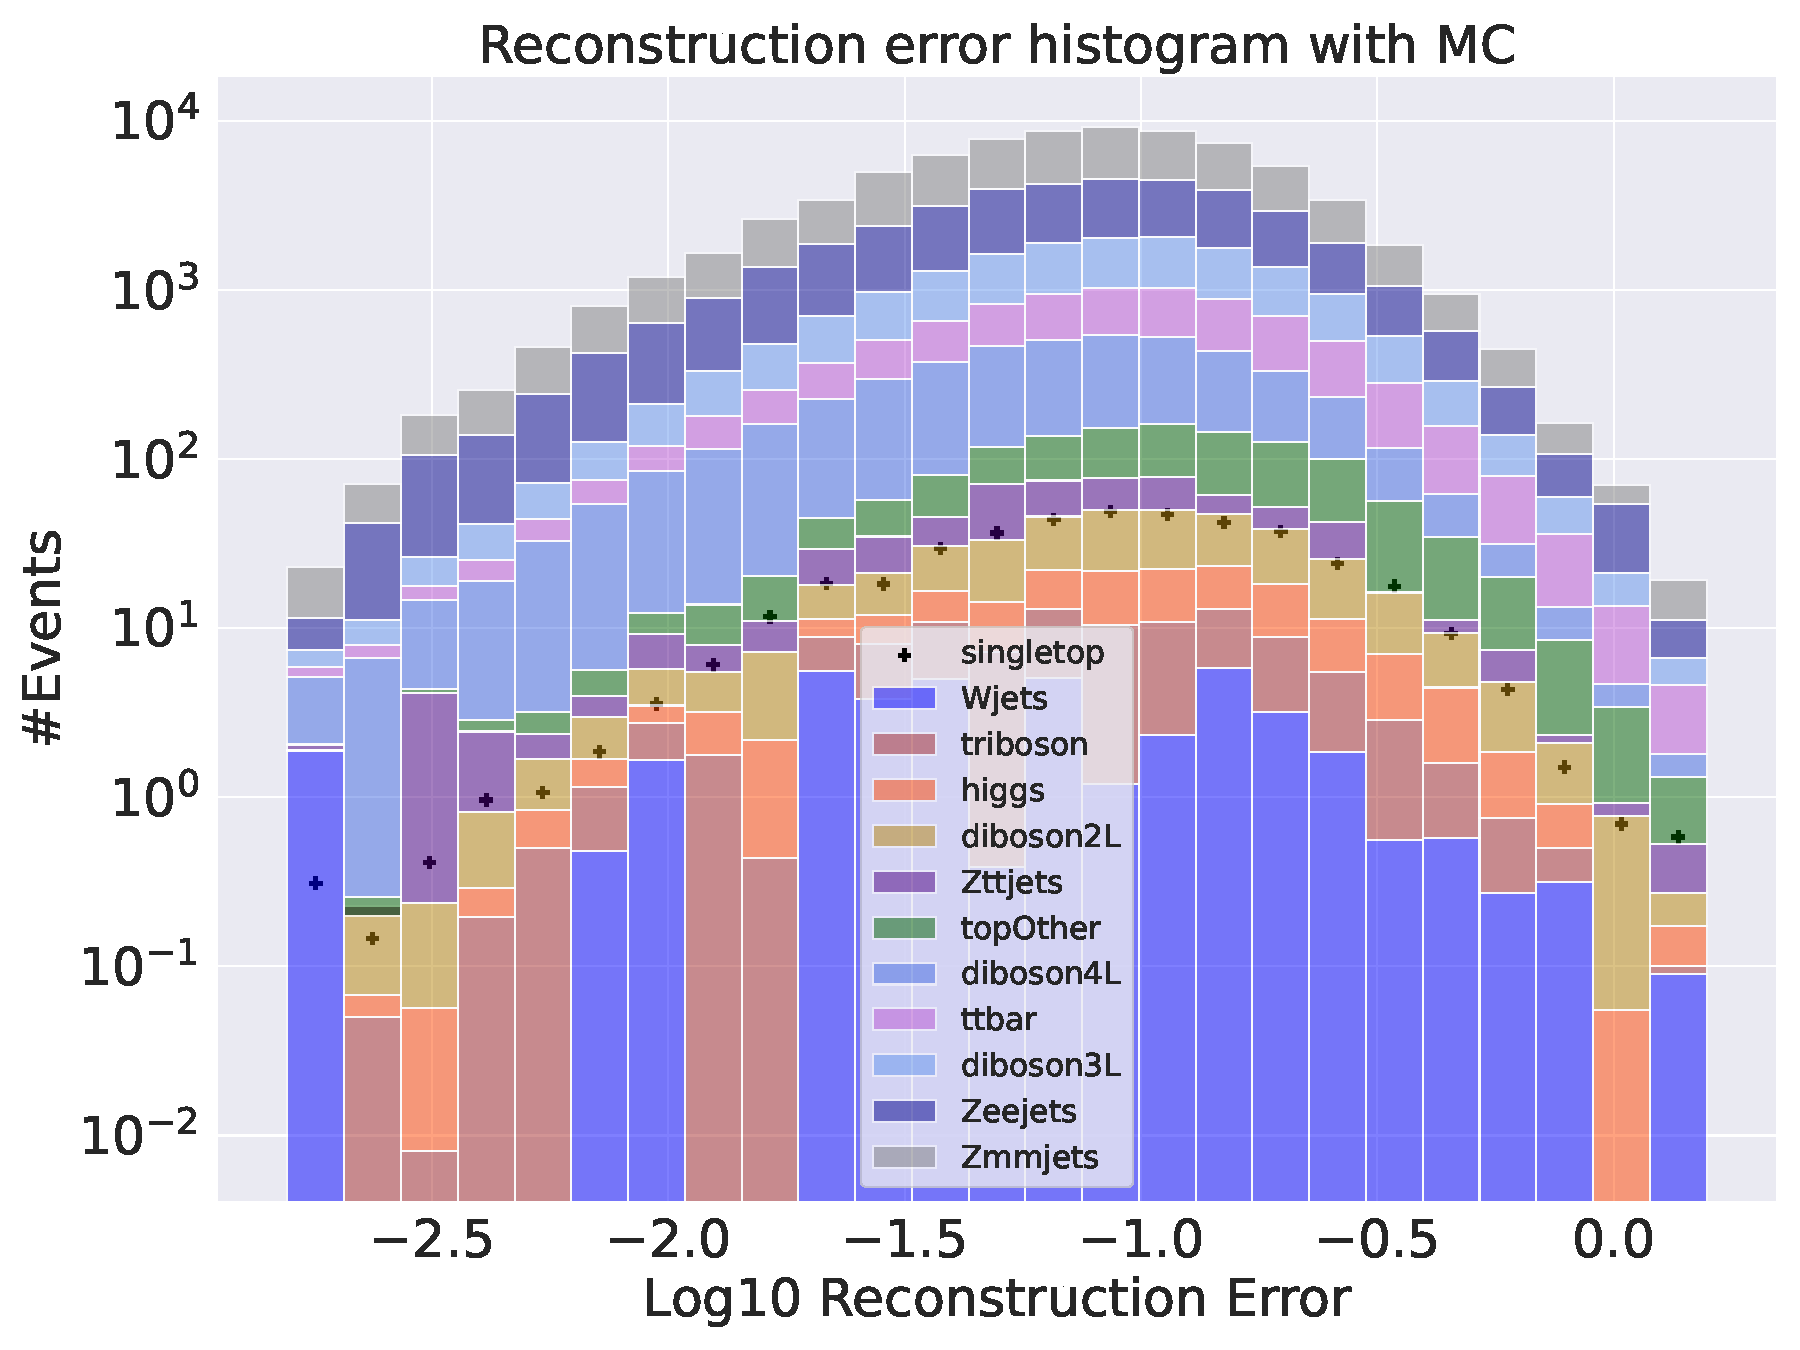
\includegraphics[width=\textwidth]{Figures/VAE_testing/small/b_data_recon_big_rm3_feats_sig_singletop.pdf}
        \caption{ }
        \label{fig:vae_small_singletop}
    \end{subfigure}
    \hfill
    \begin{subfigure}{.45\textwidth}
        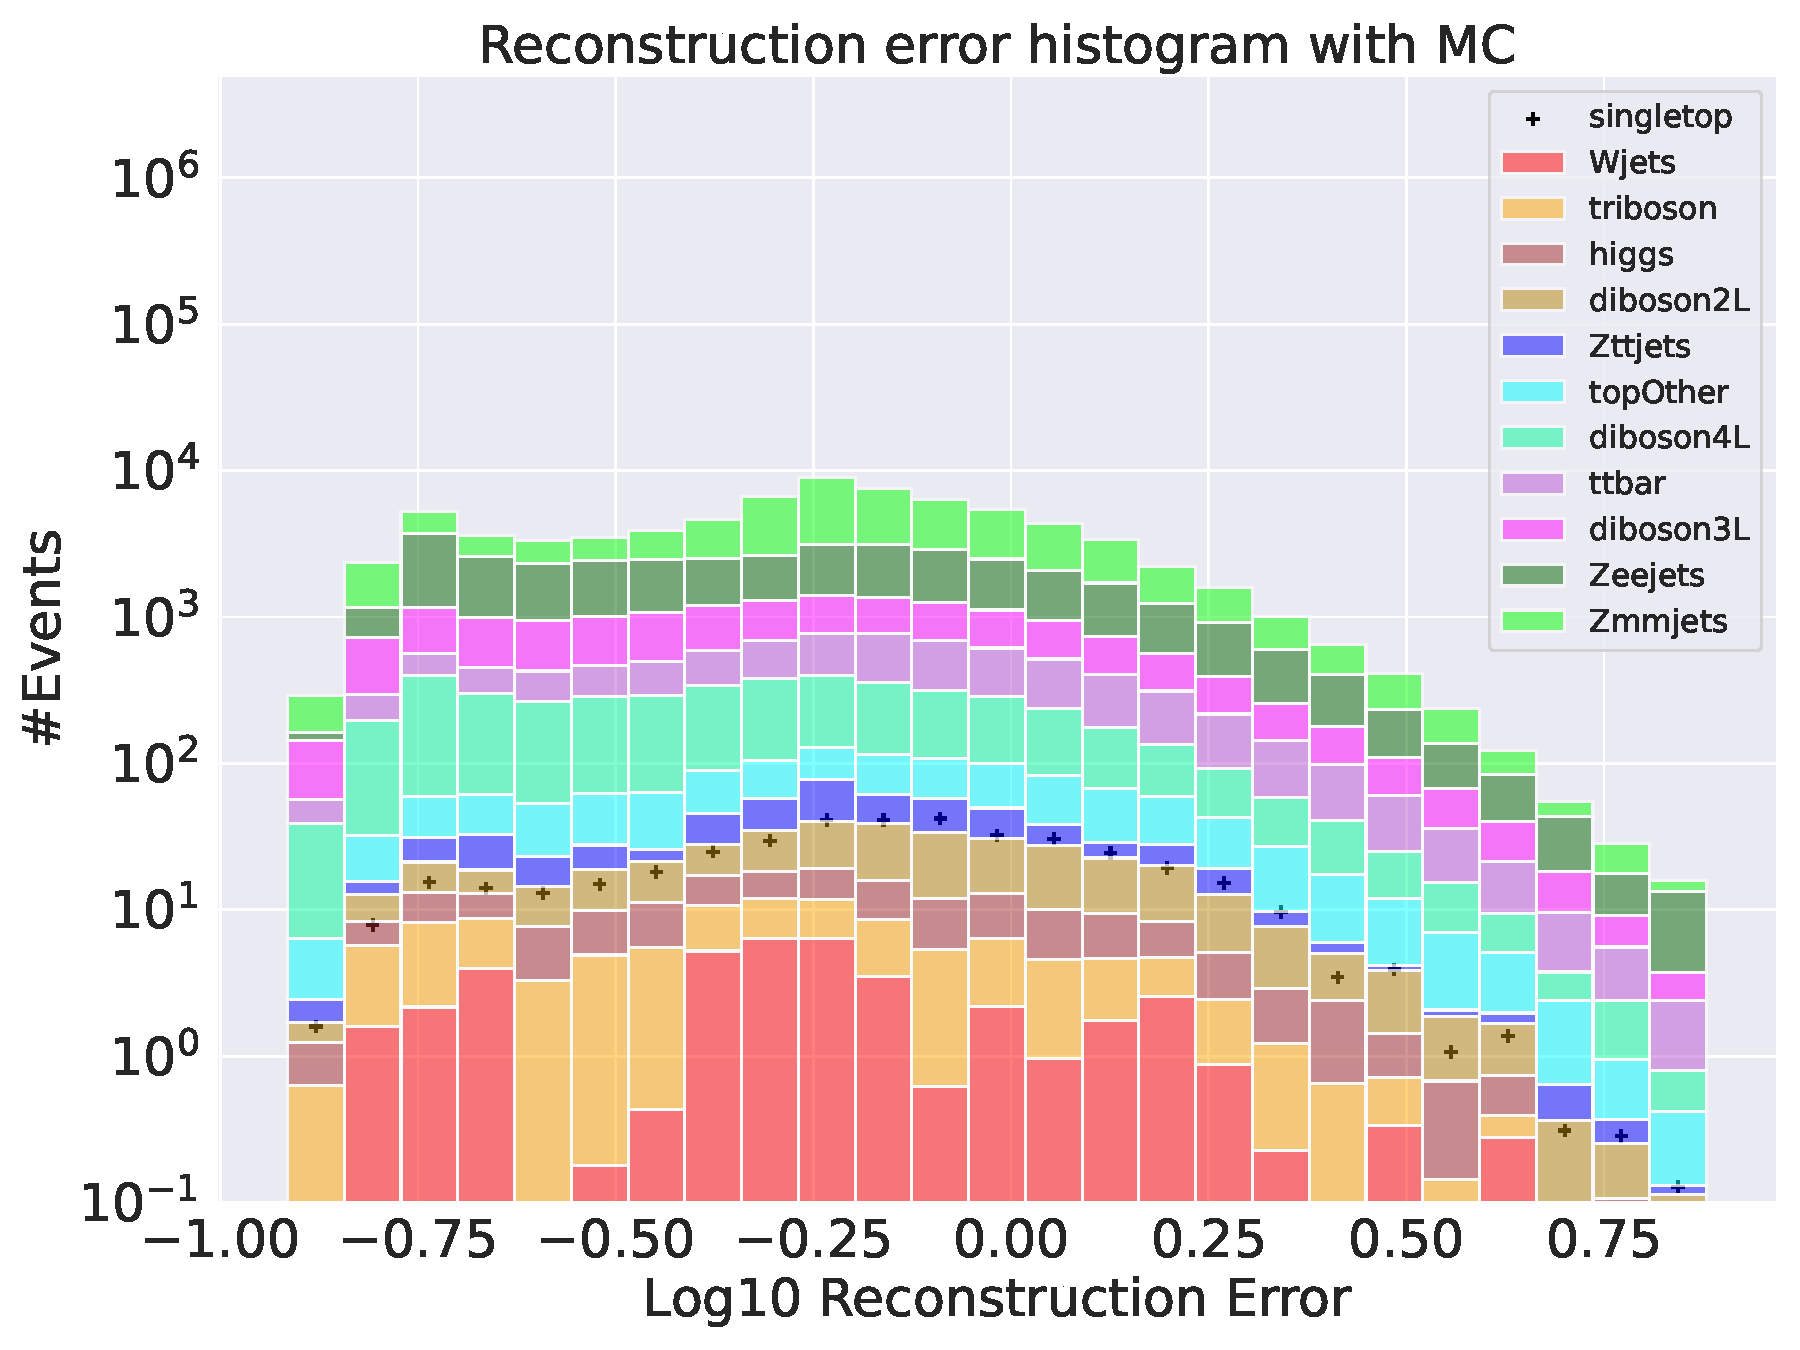
\includegraphics[width=\textwidth]{Figures/VAE_testing/big/b_data_recon_big_rm3_feats_sig_singletop.pdf}
        \caption{ }
        \label{fig:vae_big_singletop}
    \end{subfigure}
    \hfill 
    \caption[VAE | Reconstruction error using Singletop channel as signal]{Reconstruction error on validation SM MC from the small (a) and large (b) variational Autoencoder. The singletop channel has been removed from training and 
    is used as signal. No significant difference in distributions is found. }
    \label{fig:vae_big_channel_2}
\end{figure}

\begin{figure}[H]
    \centering
    \begin{subfigure}{.45\textwidth}
        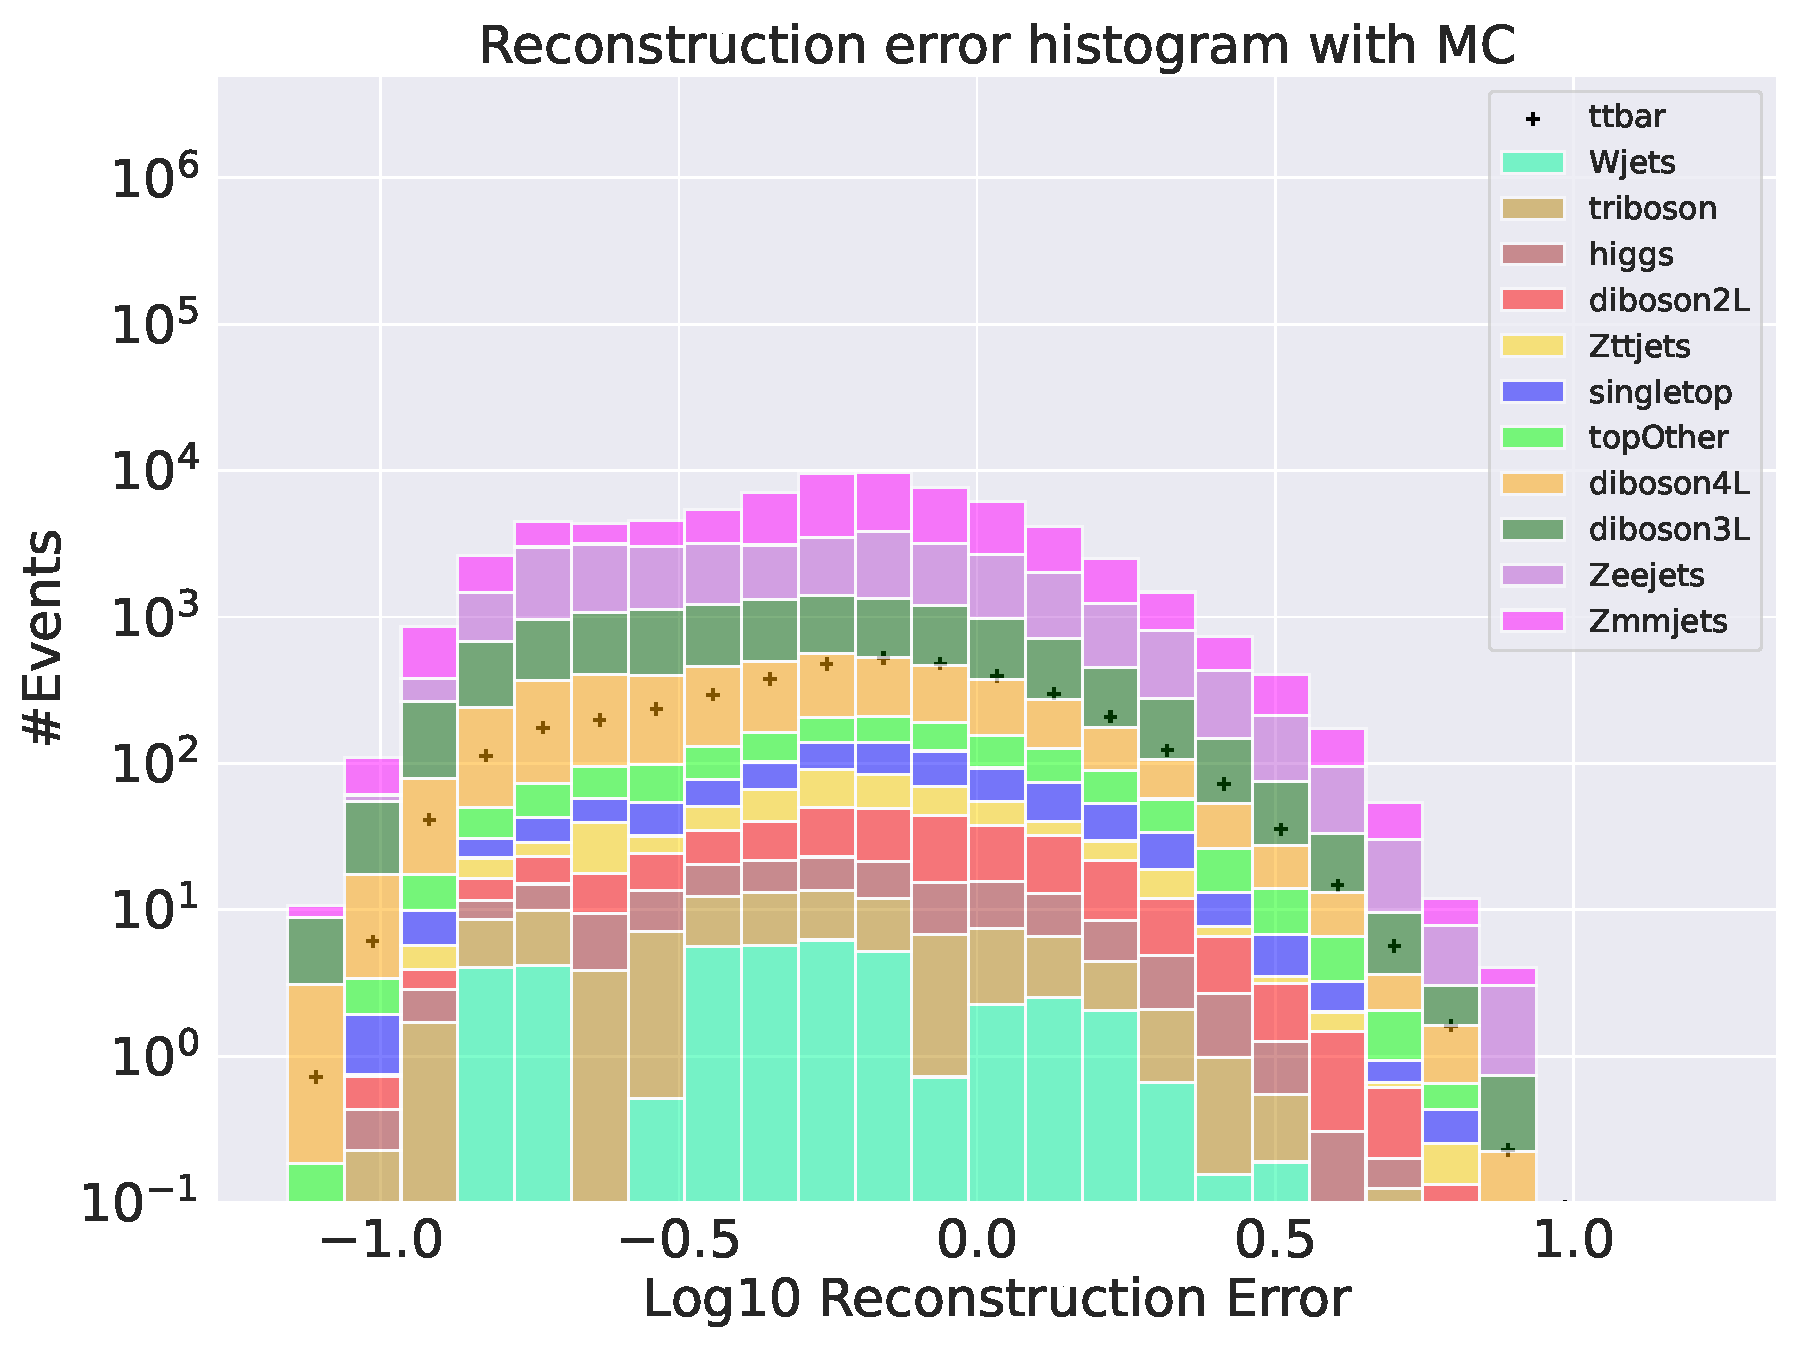
\includegraphics[width=\textwidth]{Figures/VAE_testing/small/b_data_recon_big_rm3_feats_sig_ttbar.pdf}
        \caption{}
        \label{fig:vae_small_ttbar}
    \end{subfigure}
    \hfill 
    \begin{subfigure}{.45\textwidth}
        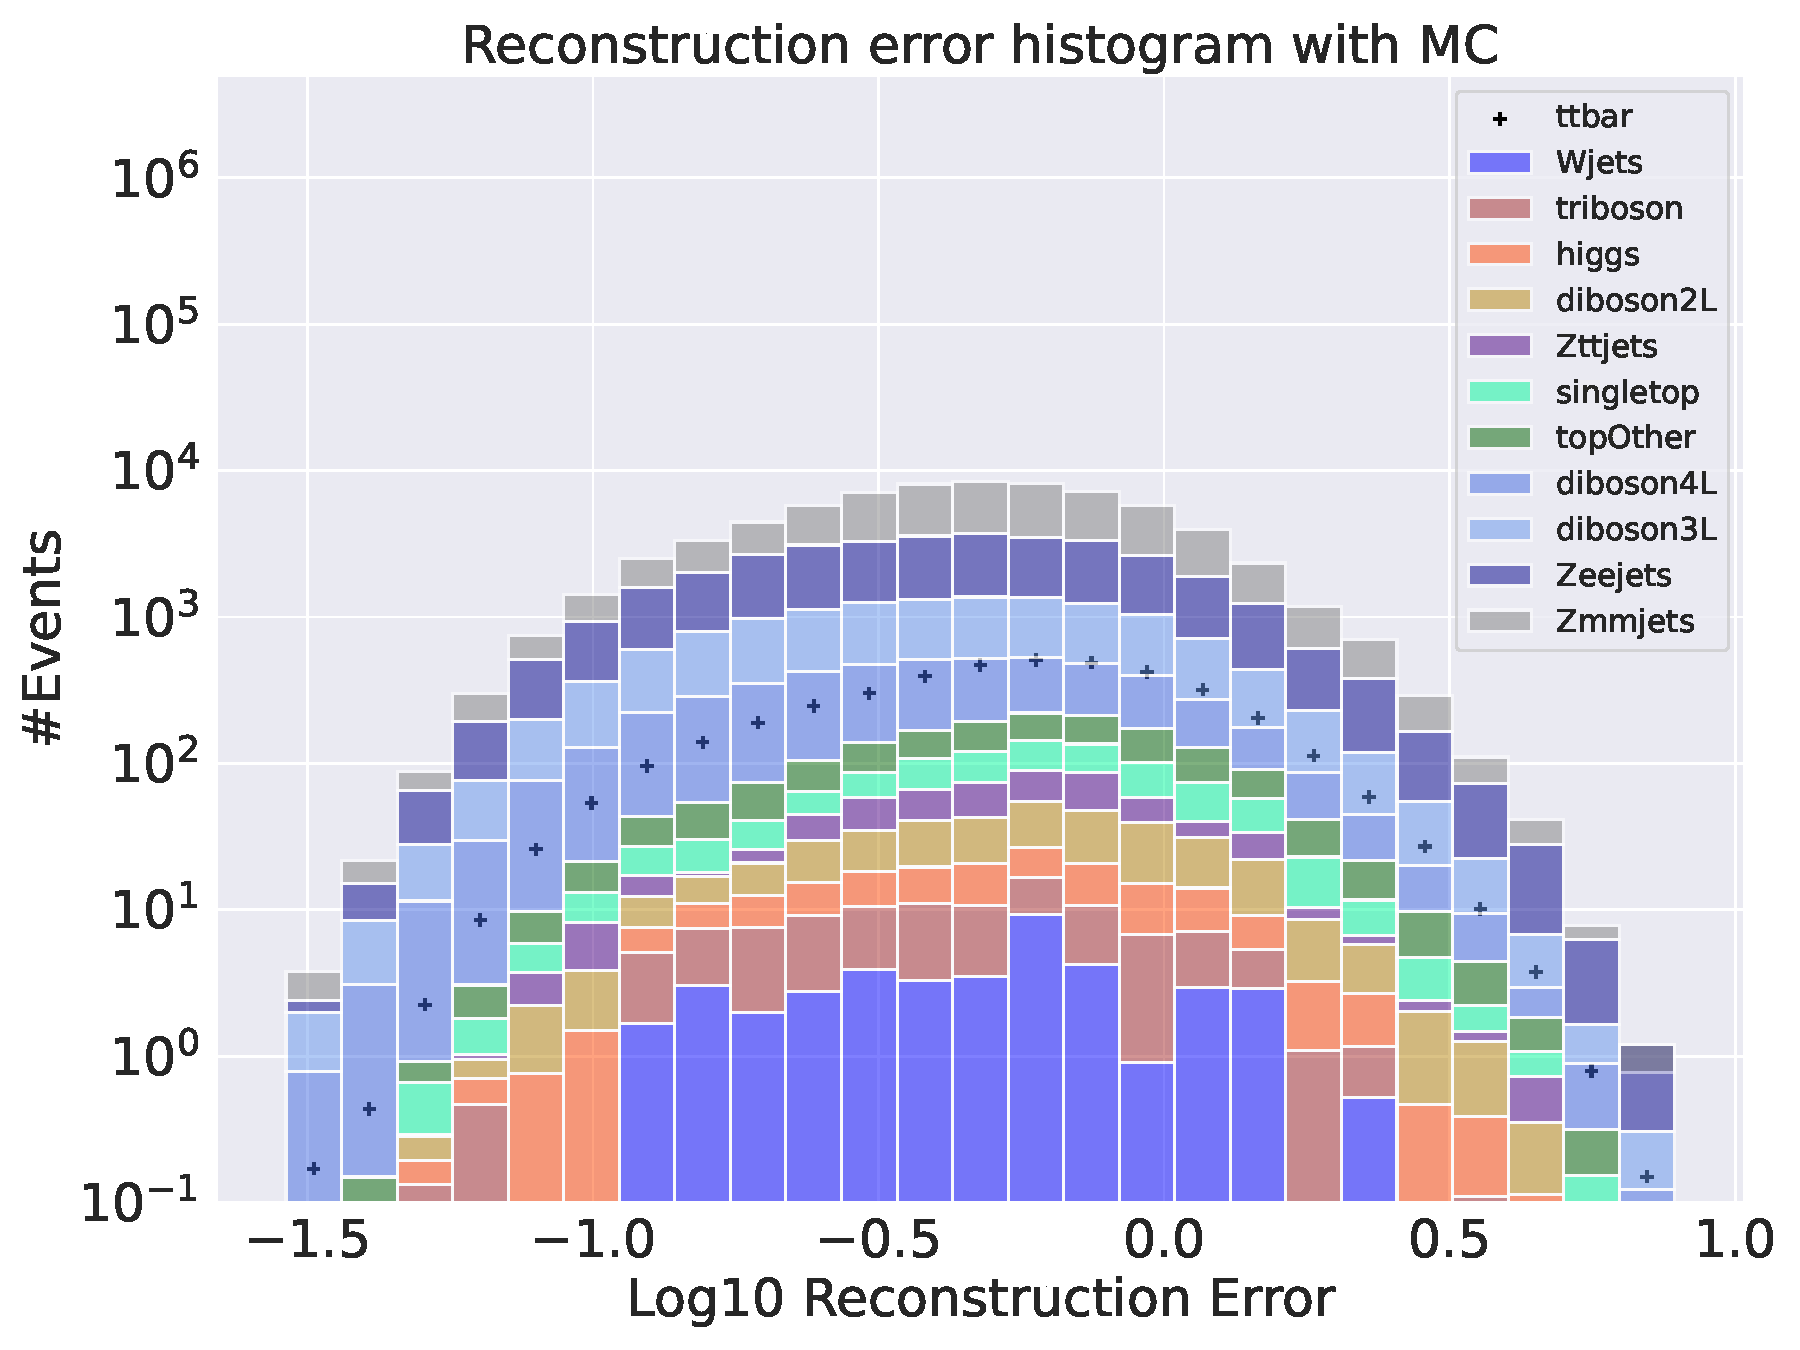
\includegraphics[width=\textwidth]{Figures/VAE_testing/big/b_data_recon_big_rm3_feats_sig_ttbar.pdf}
        \caption{ }
        \label{fig:vae_big_ttbar}
    \end{subfigure}
    \hfill 
    \caption[VAE | Reconstruction error using ttbar channel as signal]{Reconstruction error on validation SM MC from the small (a) and large (b) variational Autoencoder. The ttbar channel has been removed from training and 
    is used as signal. No significant difference in distributions is found.  }
    \label{fig:vae_big_channel_3}
\end{figure}

In figures \ref{fig:ae_big_channel_1} to \ref{fig:vae_big_channel_3} we have the reconstruction error distributions for the SM MC using 
Higgs, singletop and ttbar as signal samples for the small (to the left) and the big (to the right) regular and variational autoencoder. 
It is clear from figures that the reconstruction error distributions for the removed SM channel and the remainding SM MC are very similar. 
The same behavior is also shown for the other channels, which can found in \hl{Appendix 2}. Although the two models struggled to get a 
separation of reconstruction error distributions, the regular autoencoder seems to have a more shifted pattern of reconstruction to lower 
values than the variational autoencoder. In fact, the regular autoencoder's reconstruction error distribution peak is about 3 order of 
magnitude lower than the variational autoencoder's error distribution peak. There could be several reasons for this, one of which is that 
the variational autoencoder requires more input data to approximate the distribution, as well as the fact that the balance between the KL divergence and MSE loss 
can be difficult to handle\cite{kl_mse_balance}. This can lead to poor performance of the neural network. \hl{It should be noted that although the 
three channels selected here, as well as the rest} in \hl{Appendix 2}, do not differ that much from one another, and the hopes were not high that 
the networks would be able to separate the two distributions created. However, it does provide us with a baseline, as well as insight for what 
to expect if we were to test on signals that looks a lot like some channels. 


\newpage


\subsection*{Altering of transverse momentum}
Altering the transverse momentum of some particles would in the extreme be anomalous, and the hypothesis was that some of those trends would be
picked up by the autoencoder. Several scales for the transverse momentum were used, with the following results.


\begin{figure}[H]
    \centering
    \begin{subfigure}{.45\textwidth}
        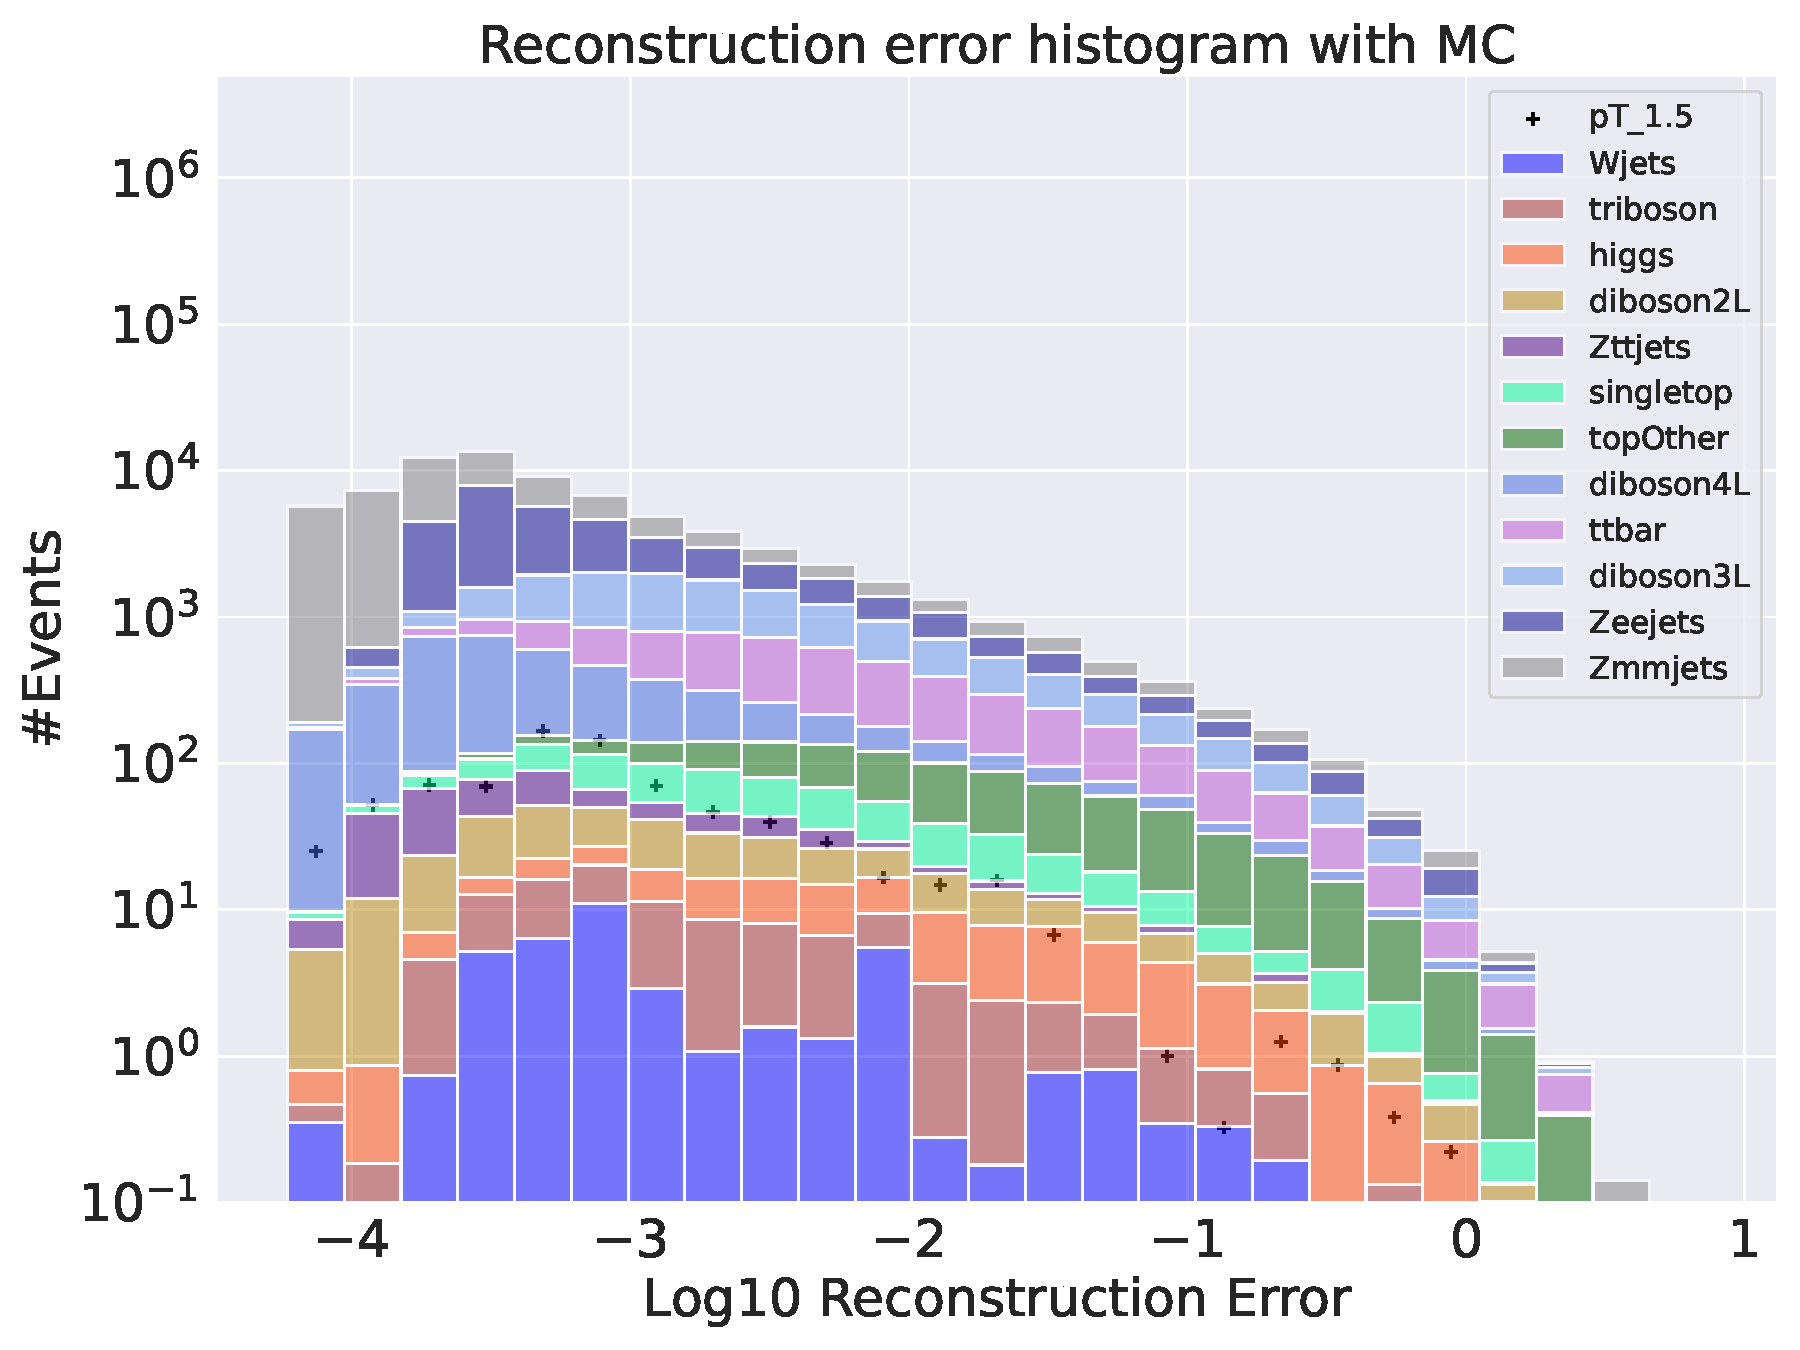
\includegraphics[width=\textwidth]{Figures/AE_testing/small/b_data_recon_big_rm3_feats_sig_pT_1.5.pdf}
        \caption{ }
        \label{fig:ae_small_pt_1_5}
    \end{subfigure}
    \hfill 
    \begin{subfigure}{.45\textwidth}
        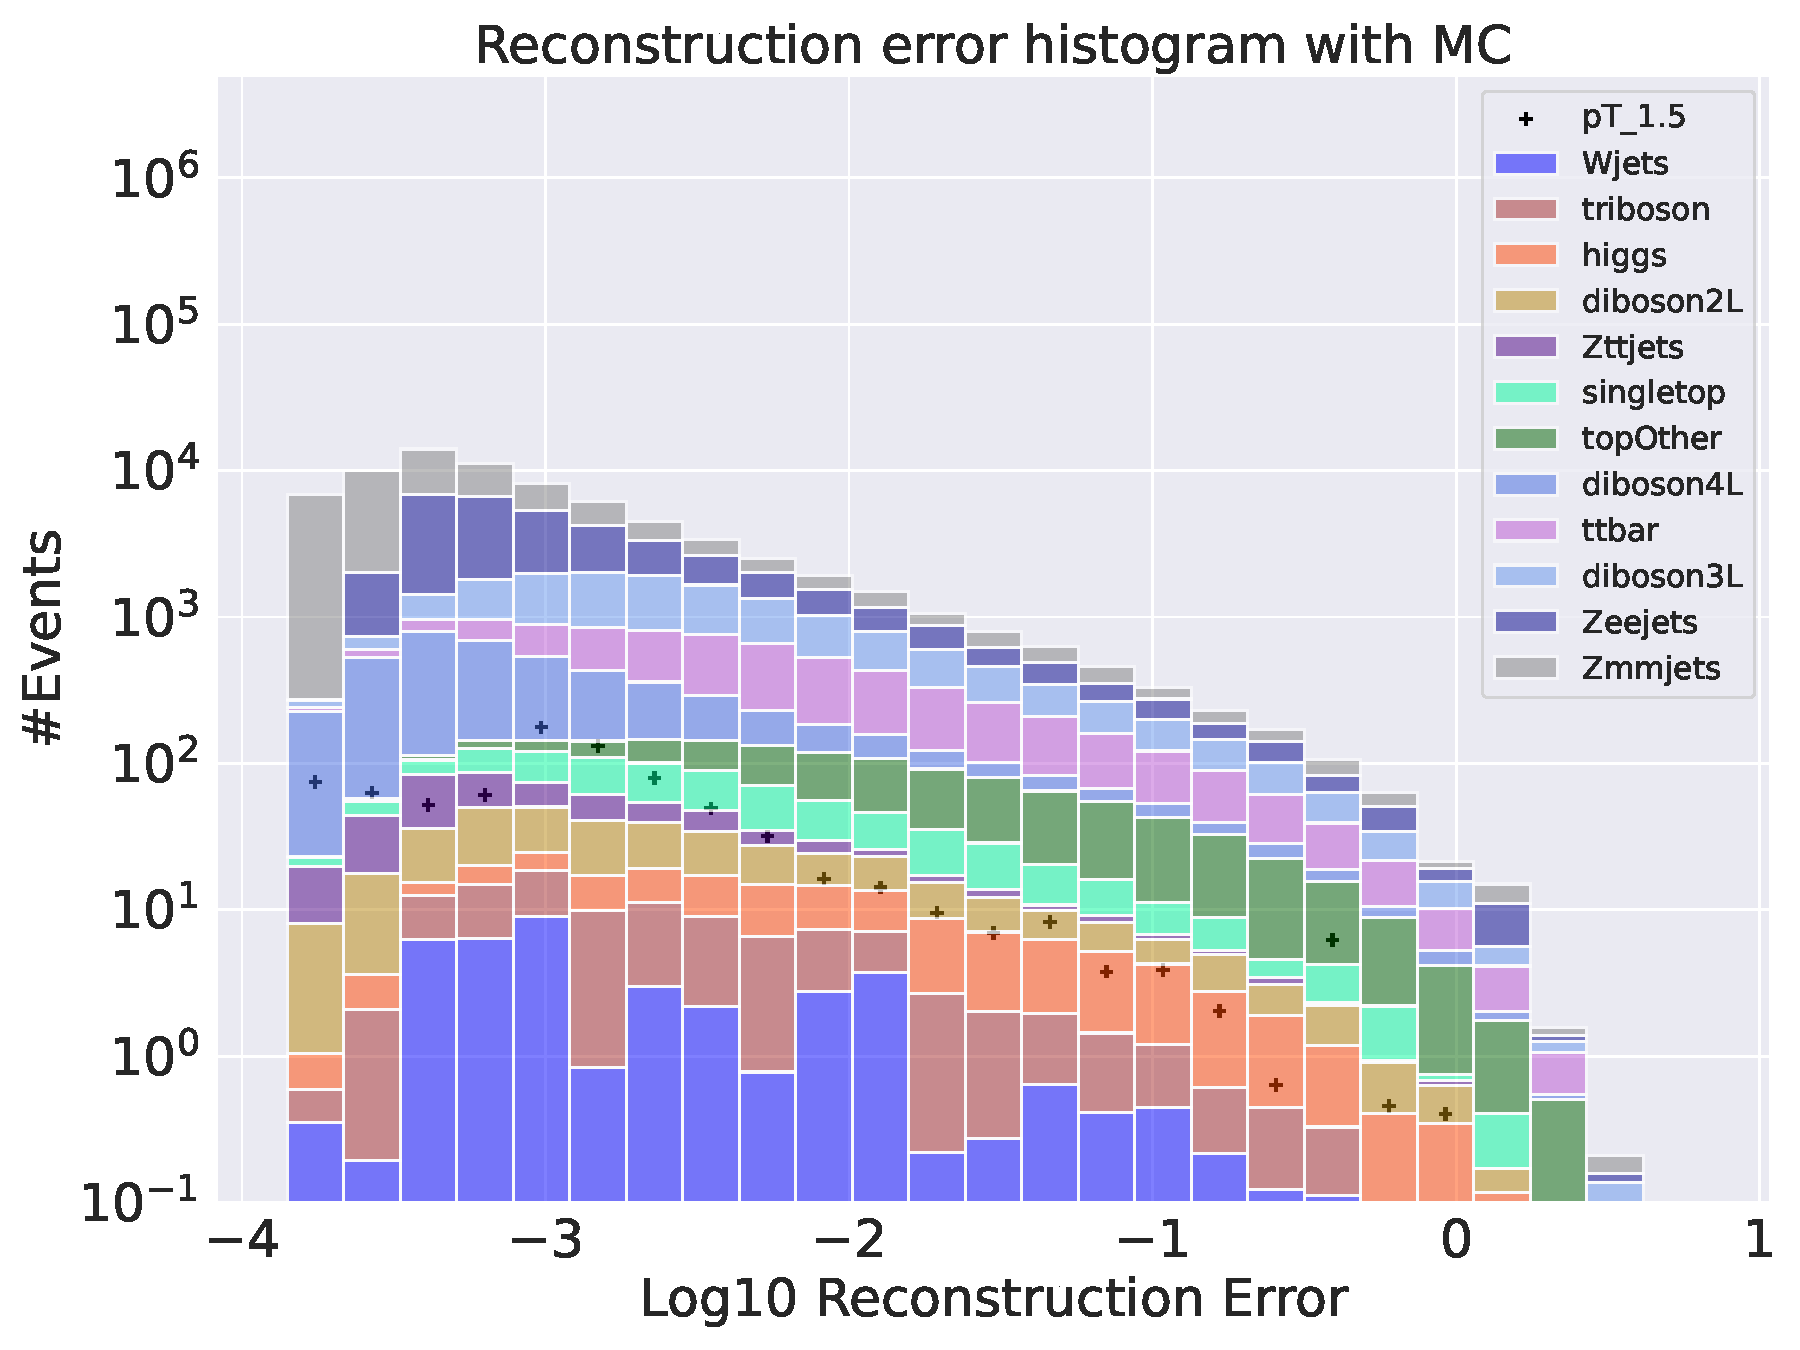
\includegraphics[width=\textwidth]{Figures/AE_testing/big/b_data_recon_big_rm3_feats_sig_pT_1.5.pdf}
        \caption{ }
        \label{fig:ae_big_pt_1_5}
    \end{subfigure}
    \hfill 
    \caption[AE | Reconstruction error $p_T$ altering of 1.5]{Reconstruction error on validation SM MC from the small (a) and large (b) regular Autoencoder. The signal is a subsample of the validation 
    set where the transverse momentum of the first electron and the first muon has been increased with a scale of $1.5$. The change of transverse 
    energy has also been changed according to the scaling of transverse momentum. No significant difference in distributions is found. }
    \label{fig:ae_big_small_pt_1_5}
\end{figure}

\begin{figure}[H]
    \centering
    \begin{subfigure}{.45\textwidth}
        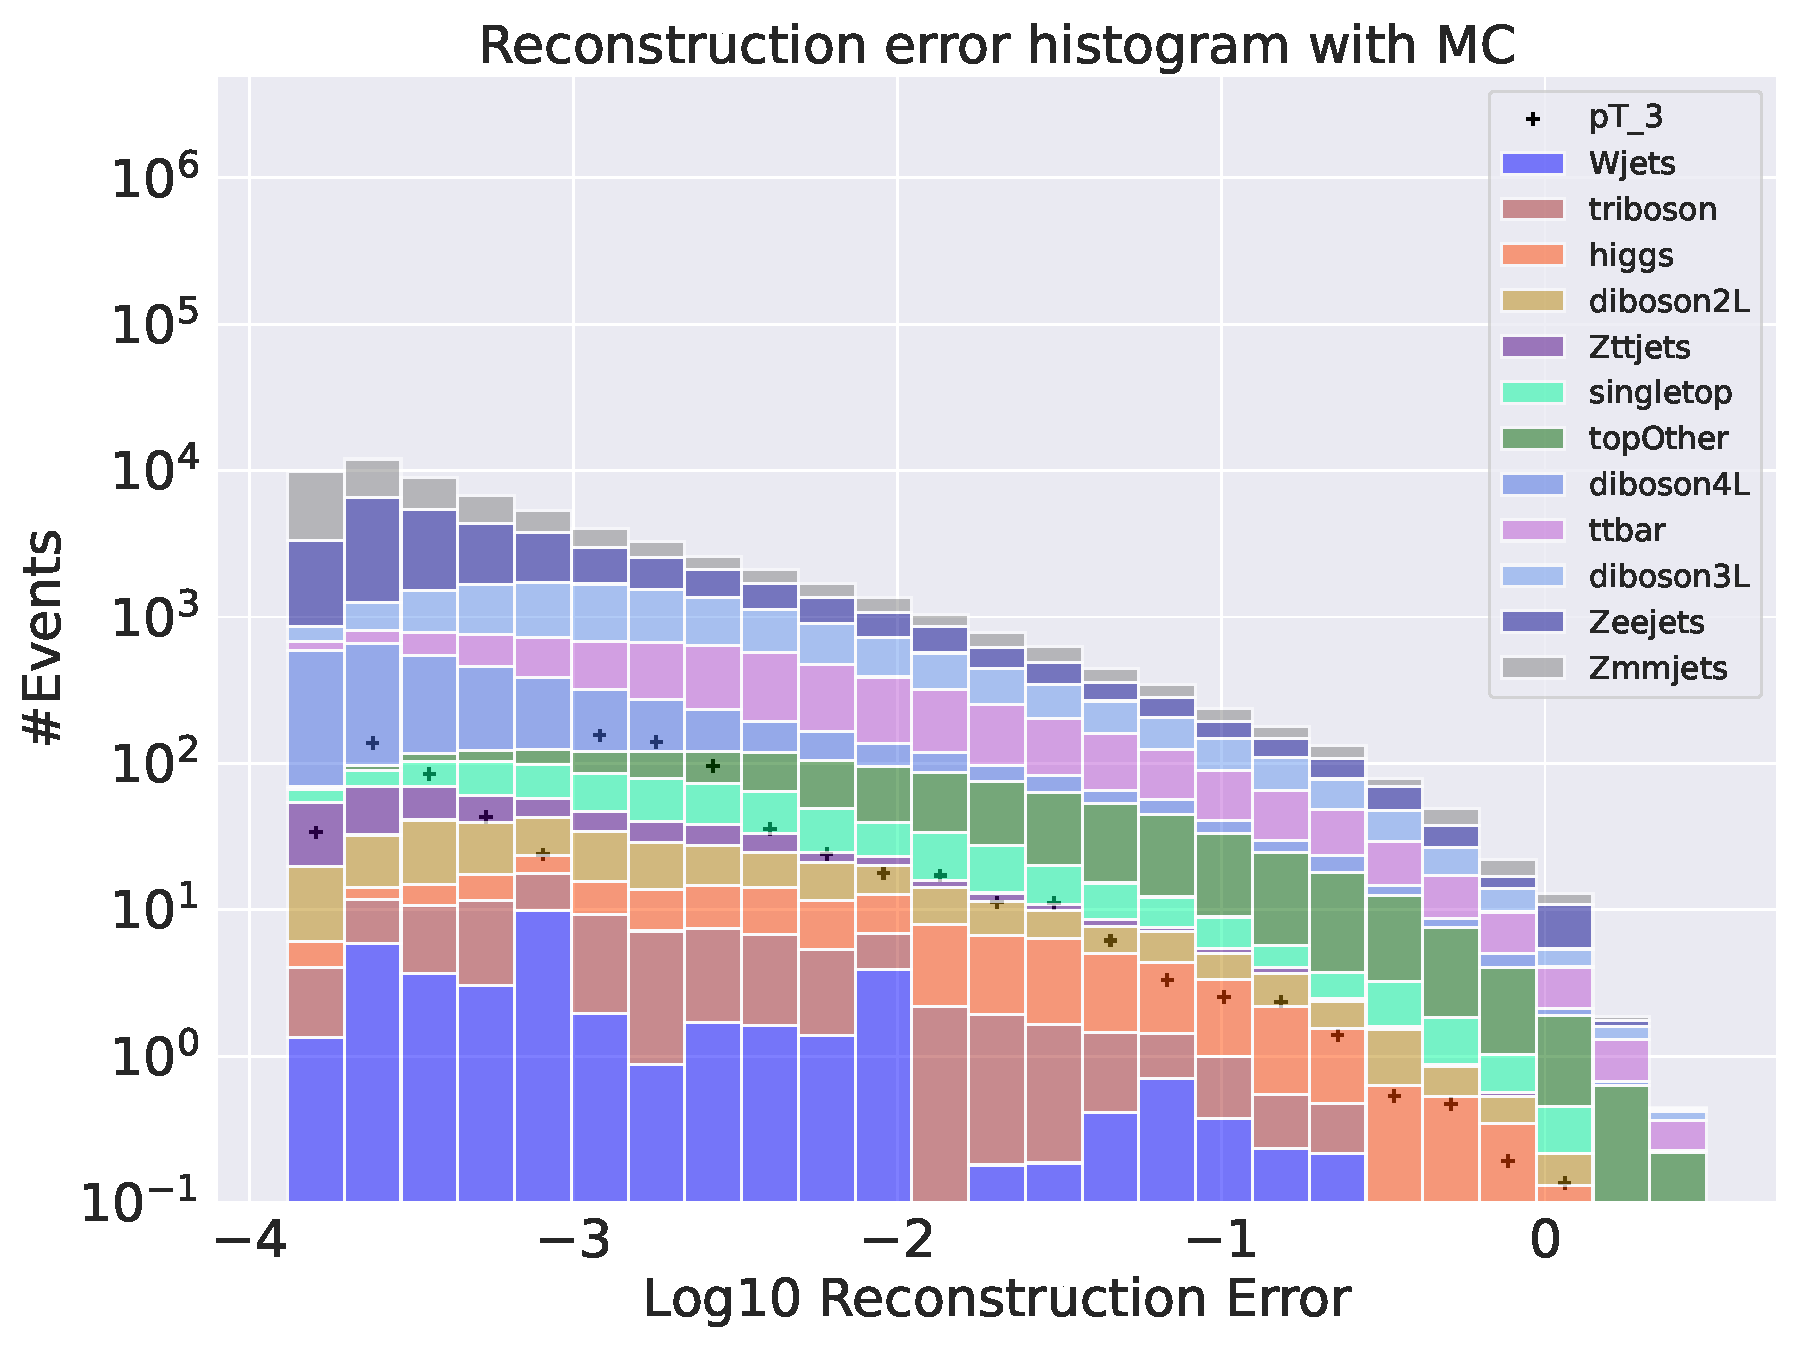
\includegraphics[width=\textwidth]{Figures/AE_testing/small/b_data_recon_big_rm3_feats_sig_pT_3.pdf}
        \caption{}
        \label{fig:ae_small_pt_3}
    \end{subfigure}
    \hfill 
    \begin{subfigure}{.45\textwidth}
        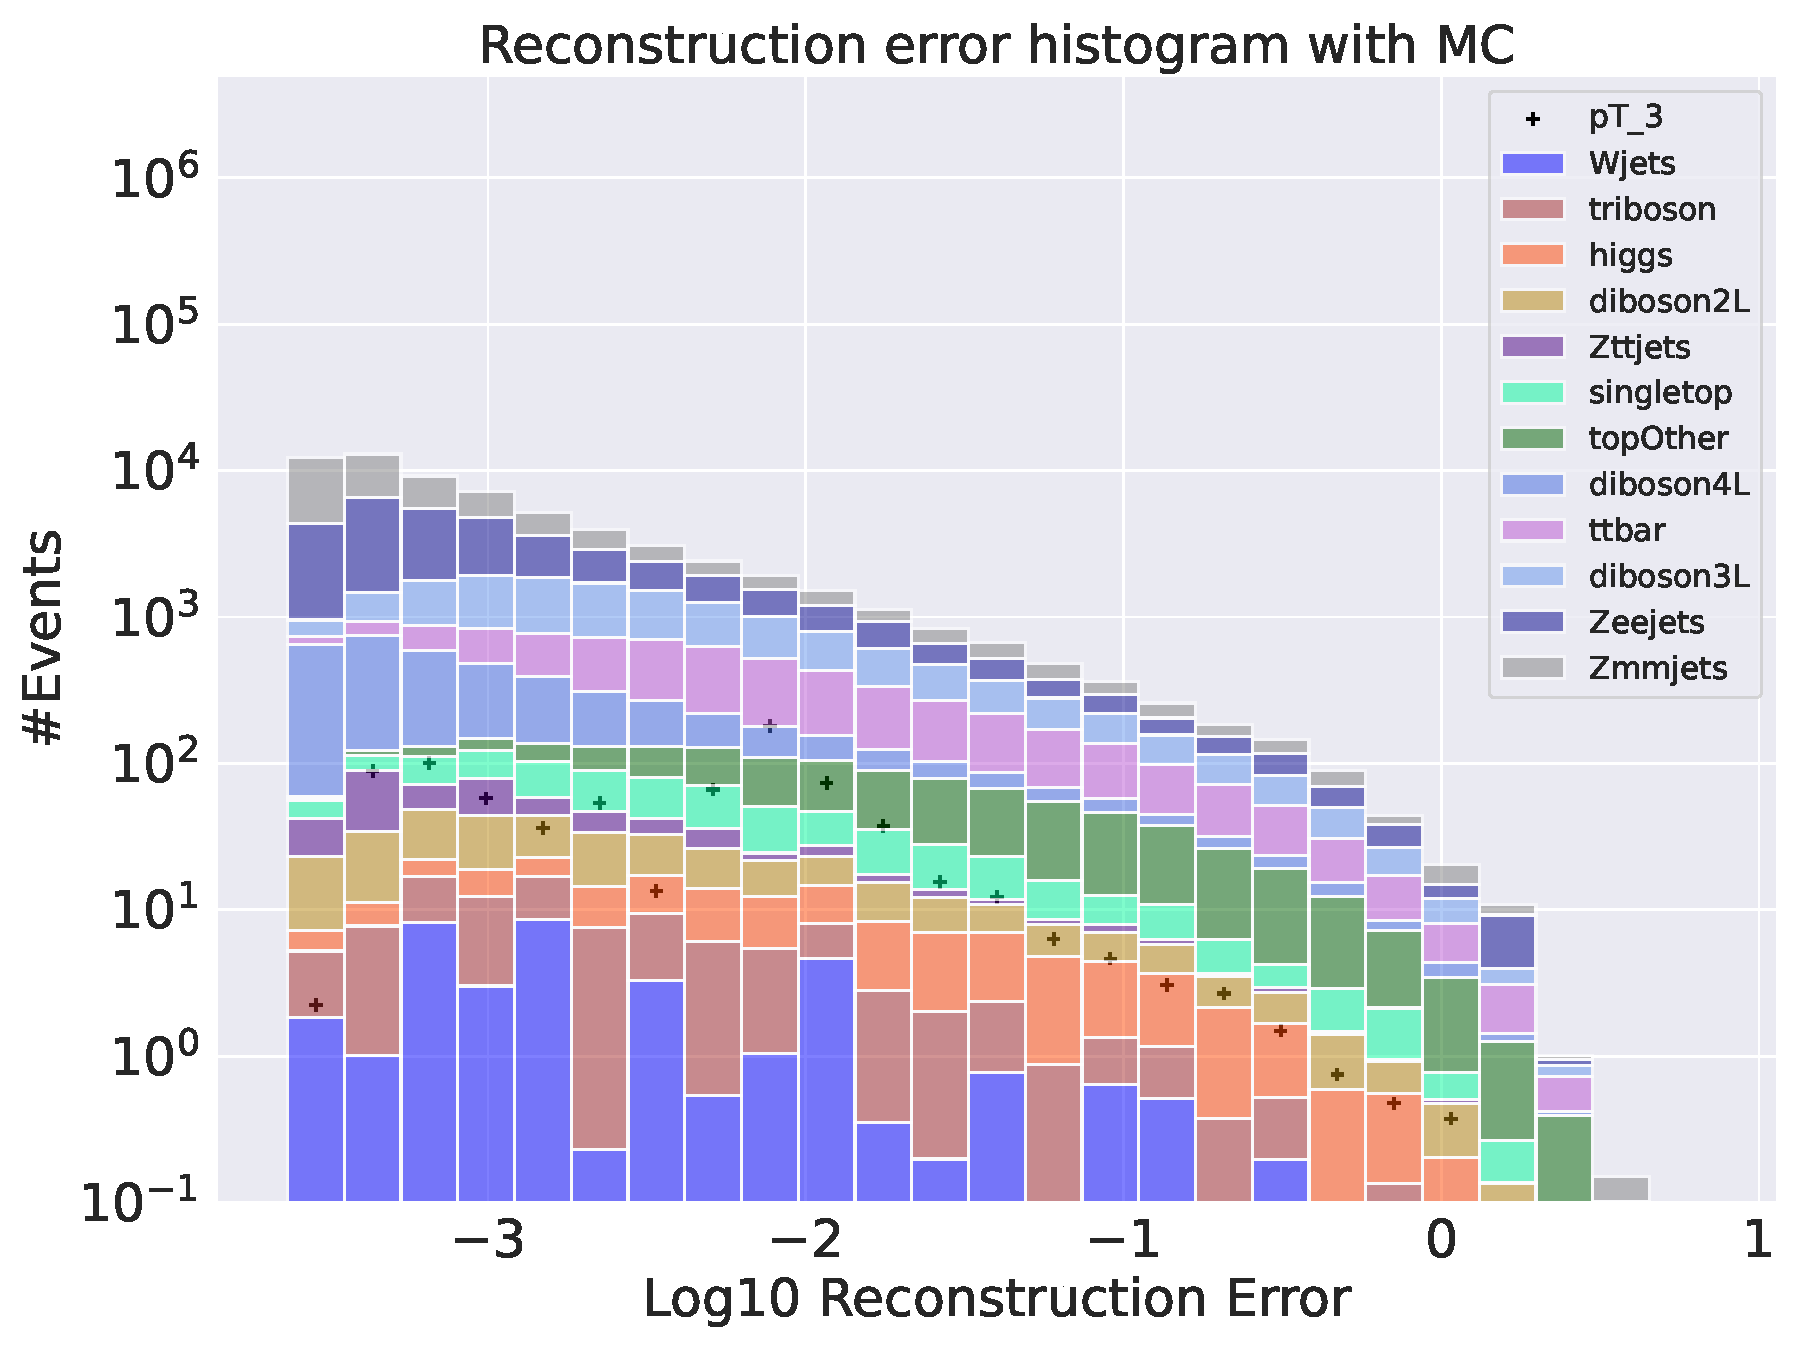
\includegraphics[width=\textwidth]{Figures/AE_testing/big/b_data_recon_big_rm3_feats_sig_pT_3.pdf}
        \caption{}
        \label{fig:ae_big_pt_3}
    \end{subfigure}
    \hfill 
    \caption[AE | Reconstruction error $p_T$ altering of 3]{Reconstruction error on validation SM MC from the small (a) and large (b) regular Autoencoder. The signal is a subsample of the validation 
    set where the transverse momentum of the first electron and the first muon has been increased with a scale of $3$. The change of transverse 
    energy has also been changed according to the scaling of transverse momentum. No significant difference in distributions is found.  }
    \label{fig:ae_big_small_pt_3}
\end{figure}

\begin{figure}[H]
    \centering
    \begin{subfigure}{.45\textwidth}
        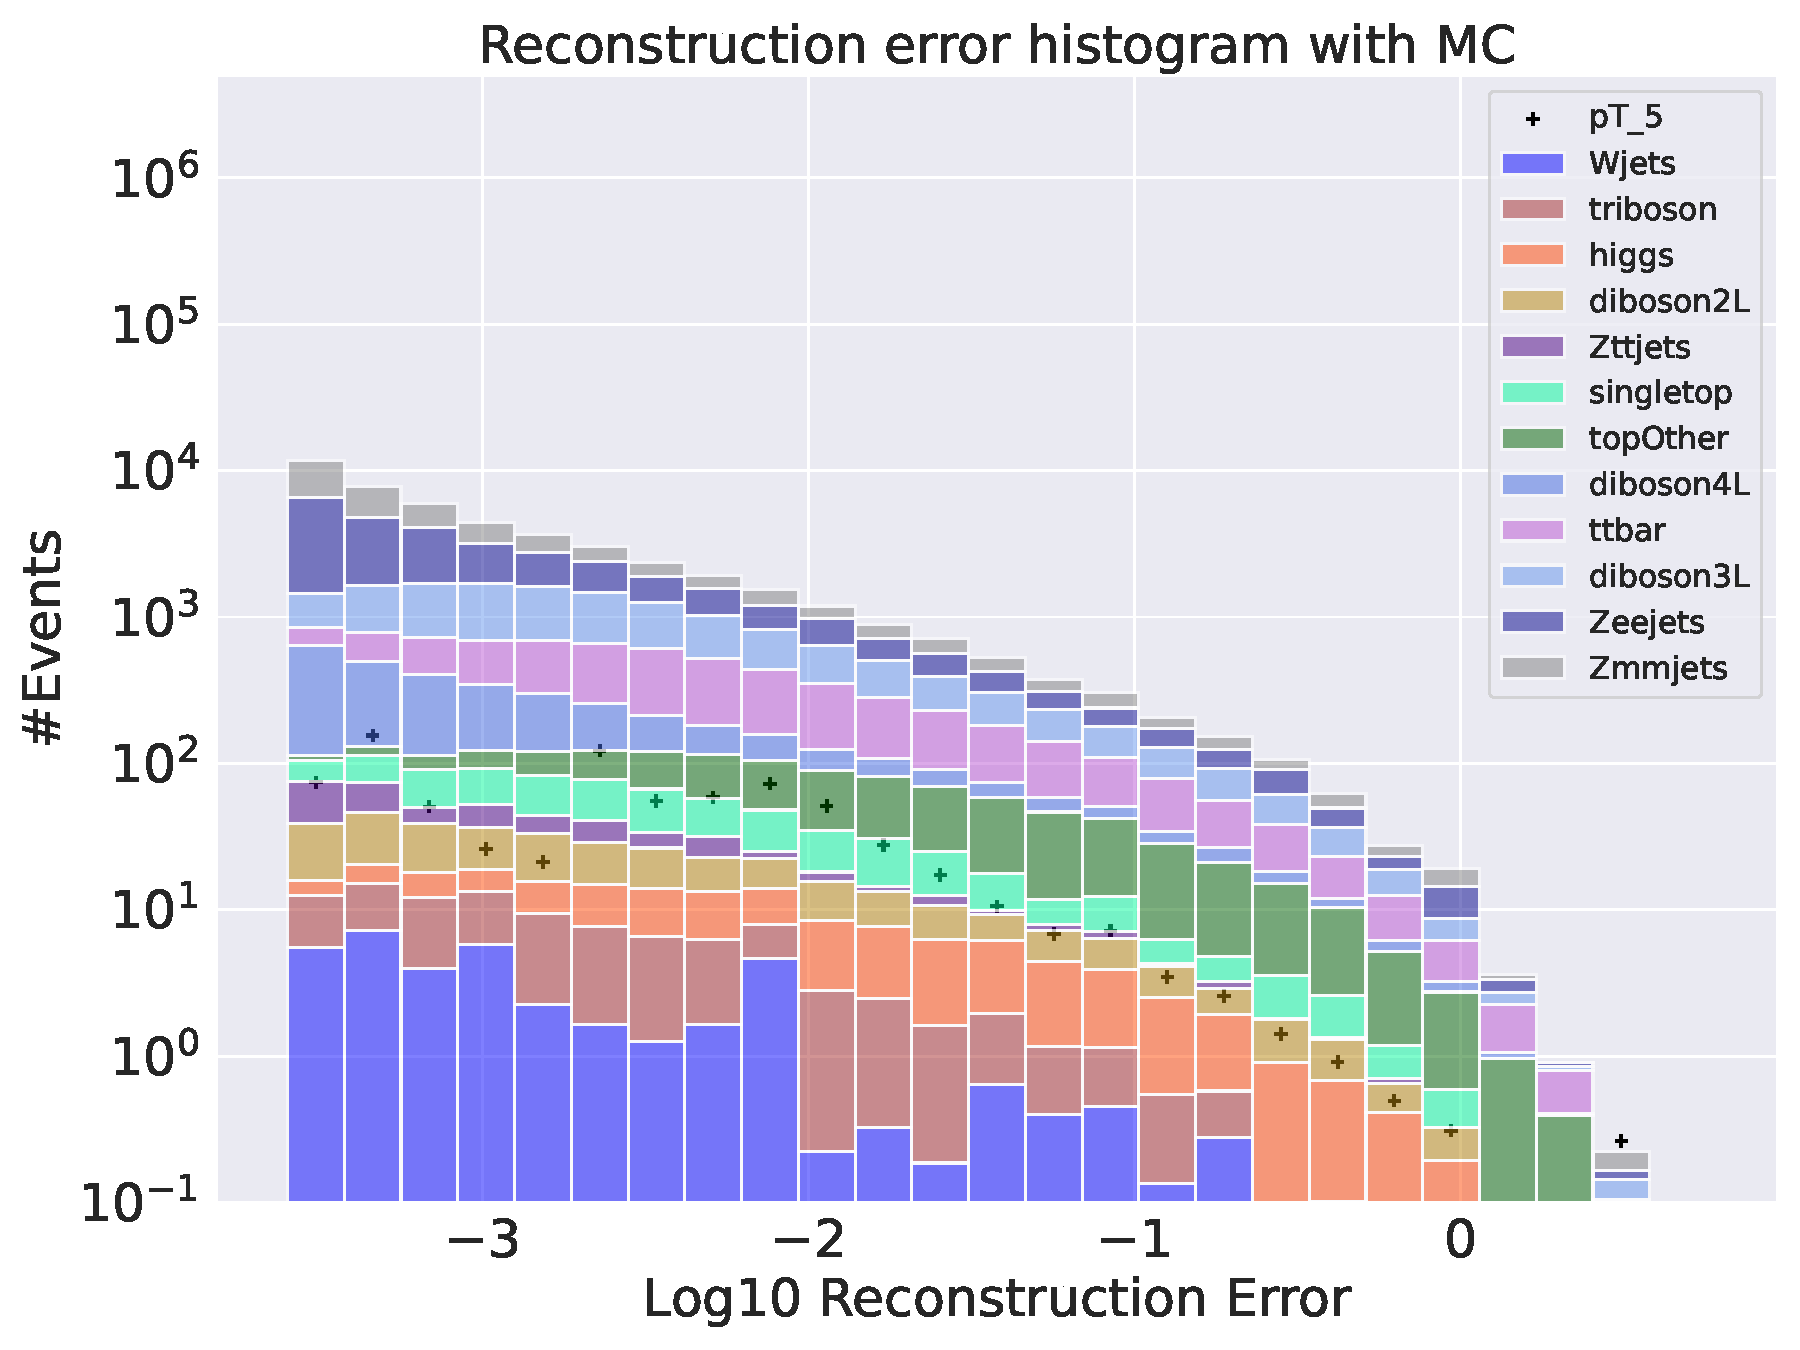
\includegraphics[width=\textwidth]{Figures/AE_testing/small/b_data_recon_big_rm3_feats_sig_pT_5.pdf}
        \caption{ }
        \label{fig:ae_small_pt_5}
    \end{subfigure}
    \hfill 
    \begin{subfigure}{.45\textwidth}
        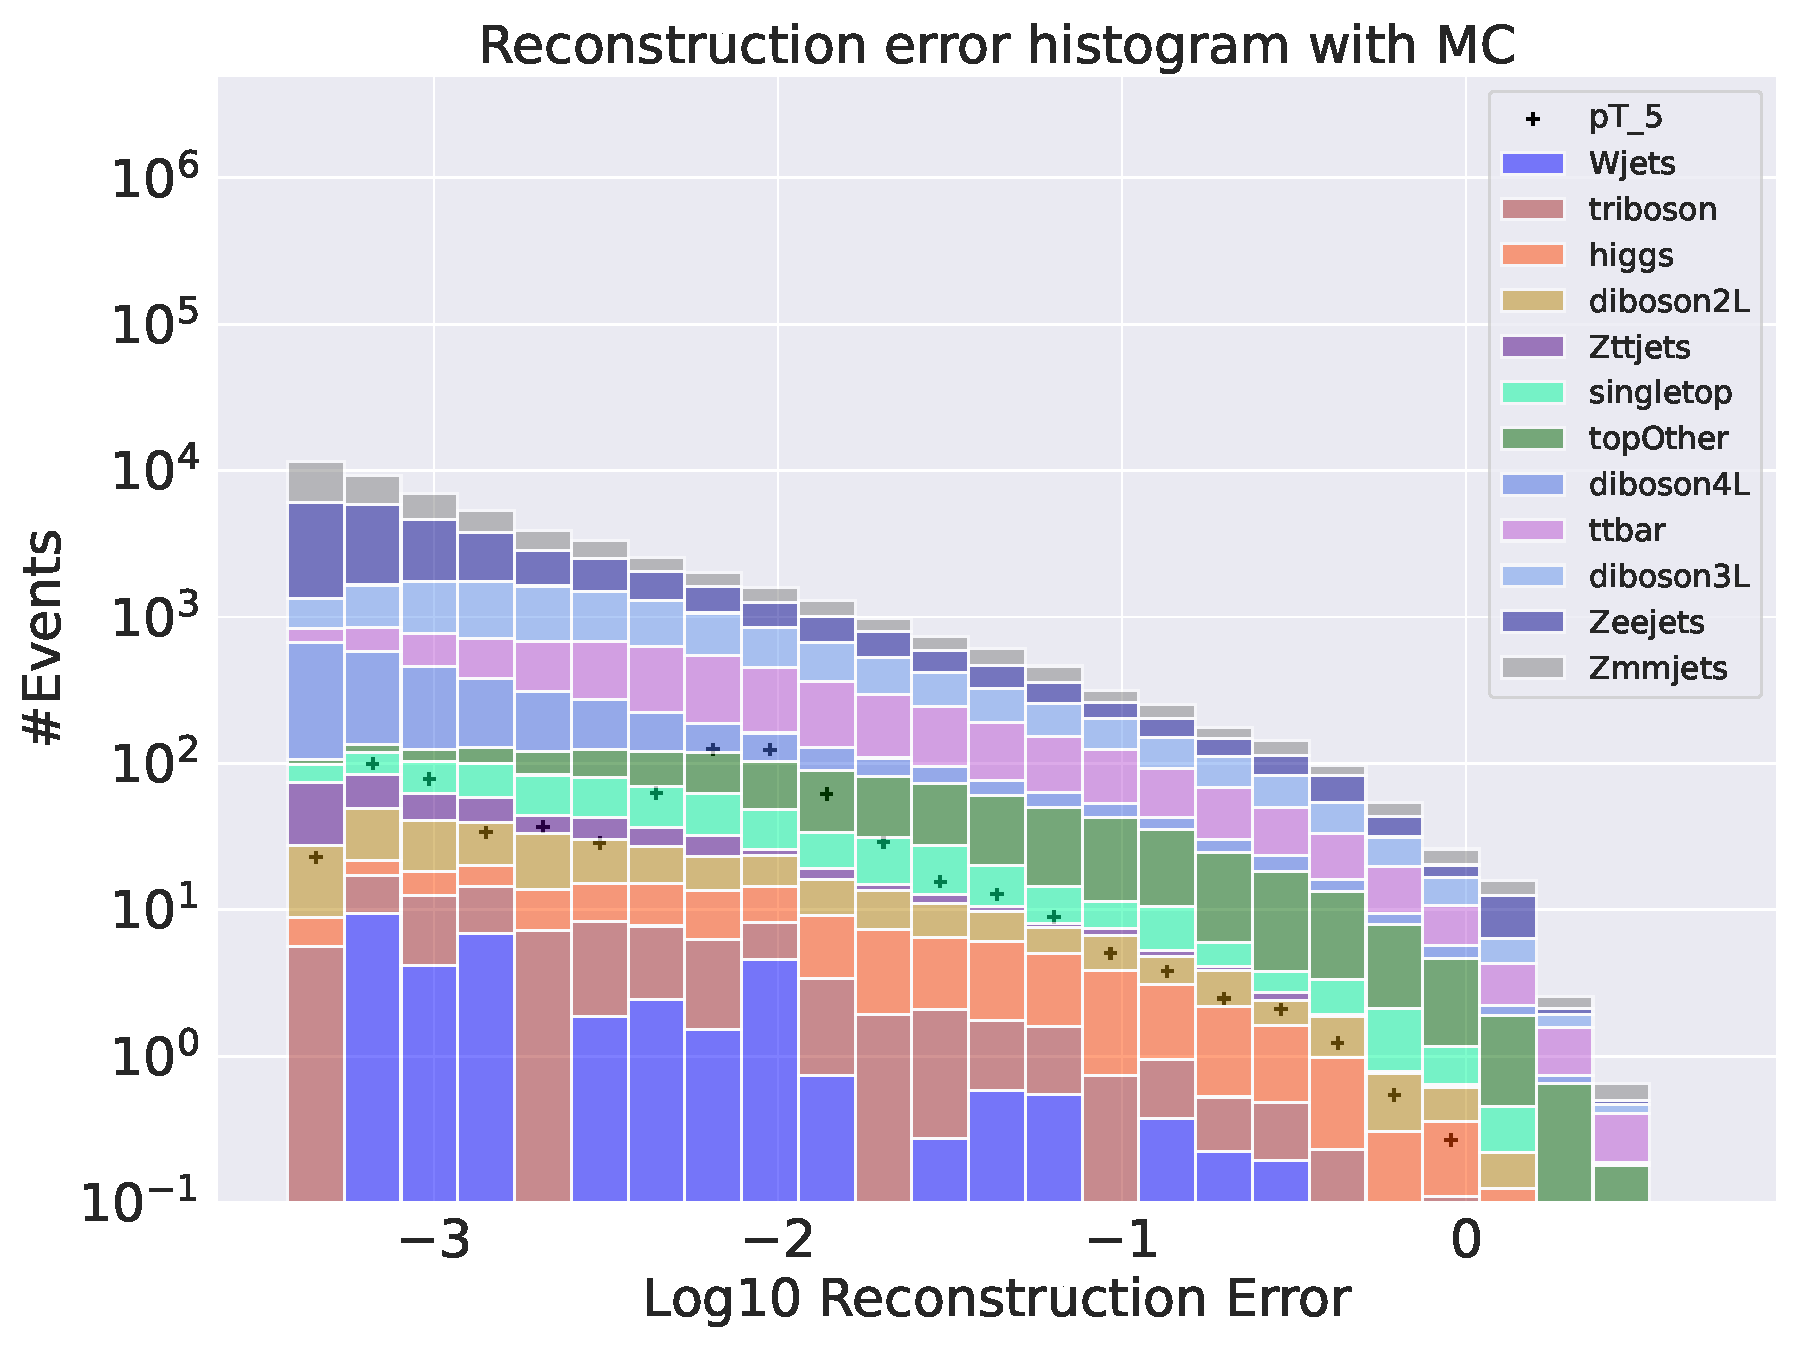
\includegraphics[width=\textwidth]{Figures/AE_testing/big/b_data_recon_big_rm3_feats_sig_pT_5.pdf}
        \caption{}
        \label{fig:ae_big_pt_5}
    \end{subfigure}
    \hfill 
    \caption[AE | Reconstruction error $p_T$ altering of 5]{Reconstruction error on validation SM MC from the small (a) and large (b) regular Autoencoder. The signal is a subsample of the validation 
    set where the transverse momentum of the first electron and the first muon has been increased with a scale of $5$. The change of transverse 
    energy has also been changed according to the scaling of transverse momentum. No significant difference in distributions is found. }
    \label{fig:ae_big_small_pt_5}
\end{figure}


\begin{figure}[H]
    \centering
    \begin{subfigure}{.45\textwidth}
        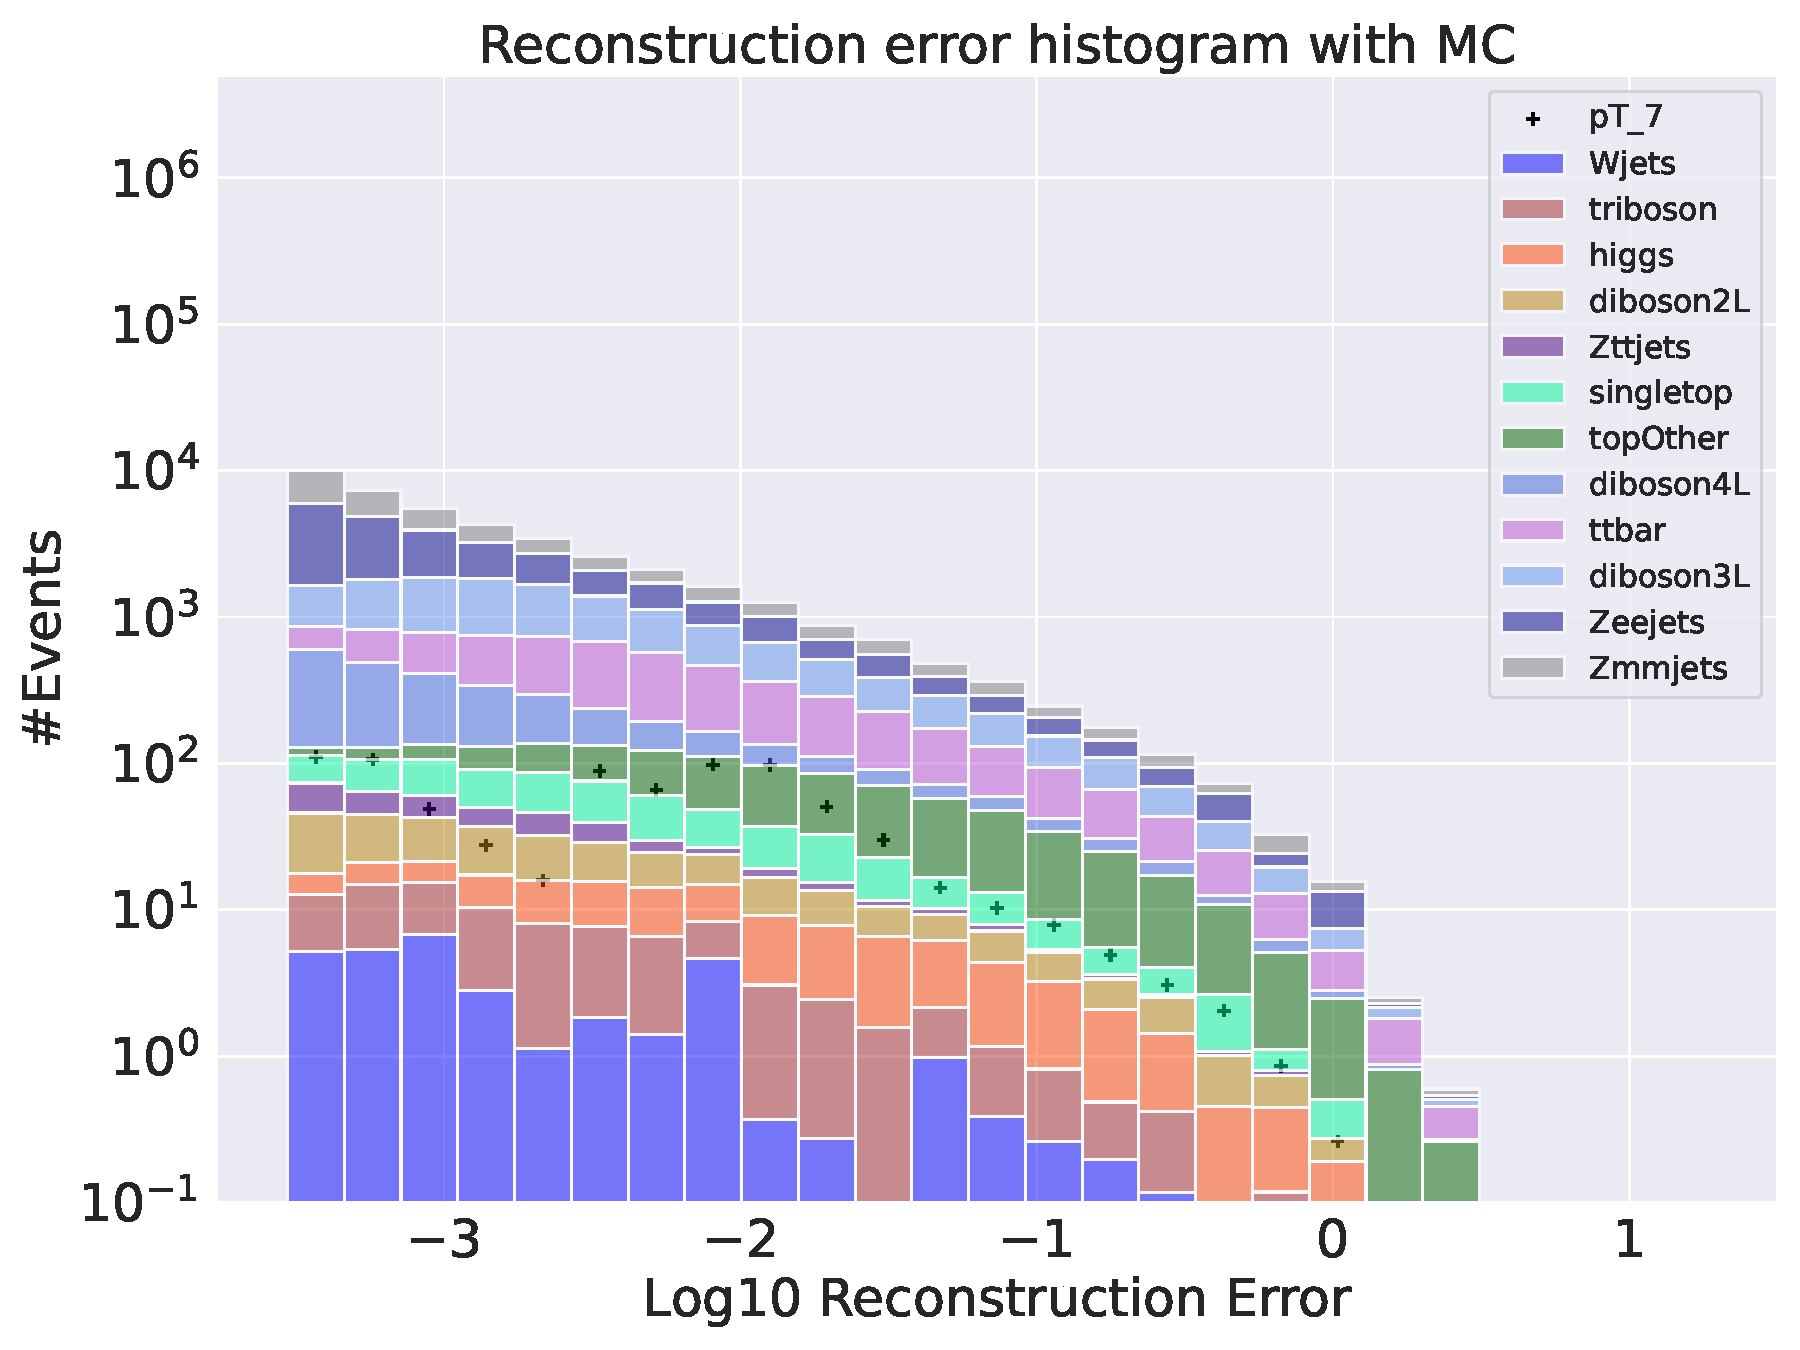
\includegraphics[width=\textwidth]{Figures/AE_testing/small/b_data_recon_big_rm3_feats_sig_pT_7.pdf}
        \caption{ }
        \label{fig:ae_small_pt_7}
    \end{subfigure}
    \hfill 
    \begin{subfigure}{.45\textwidth}
        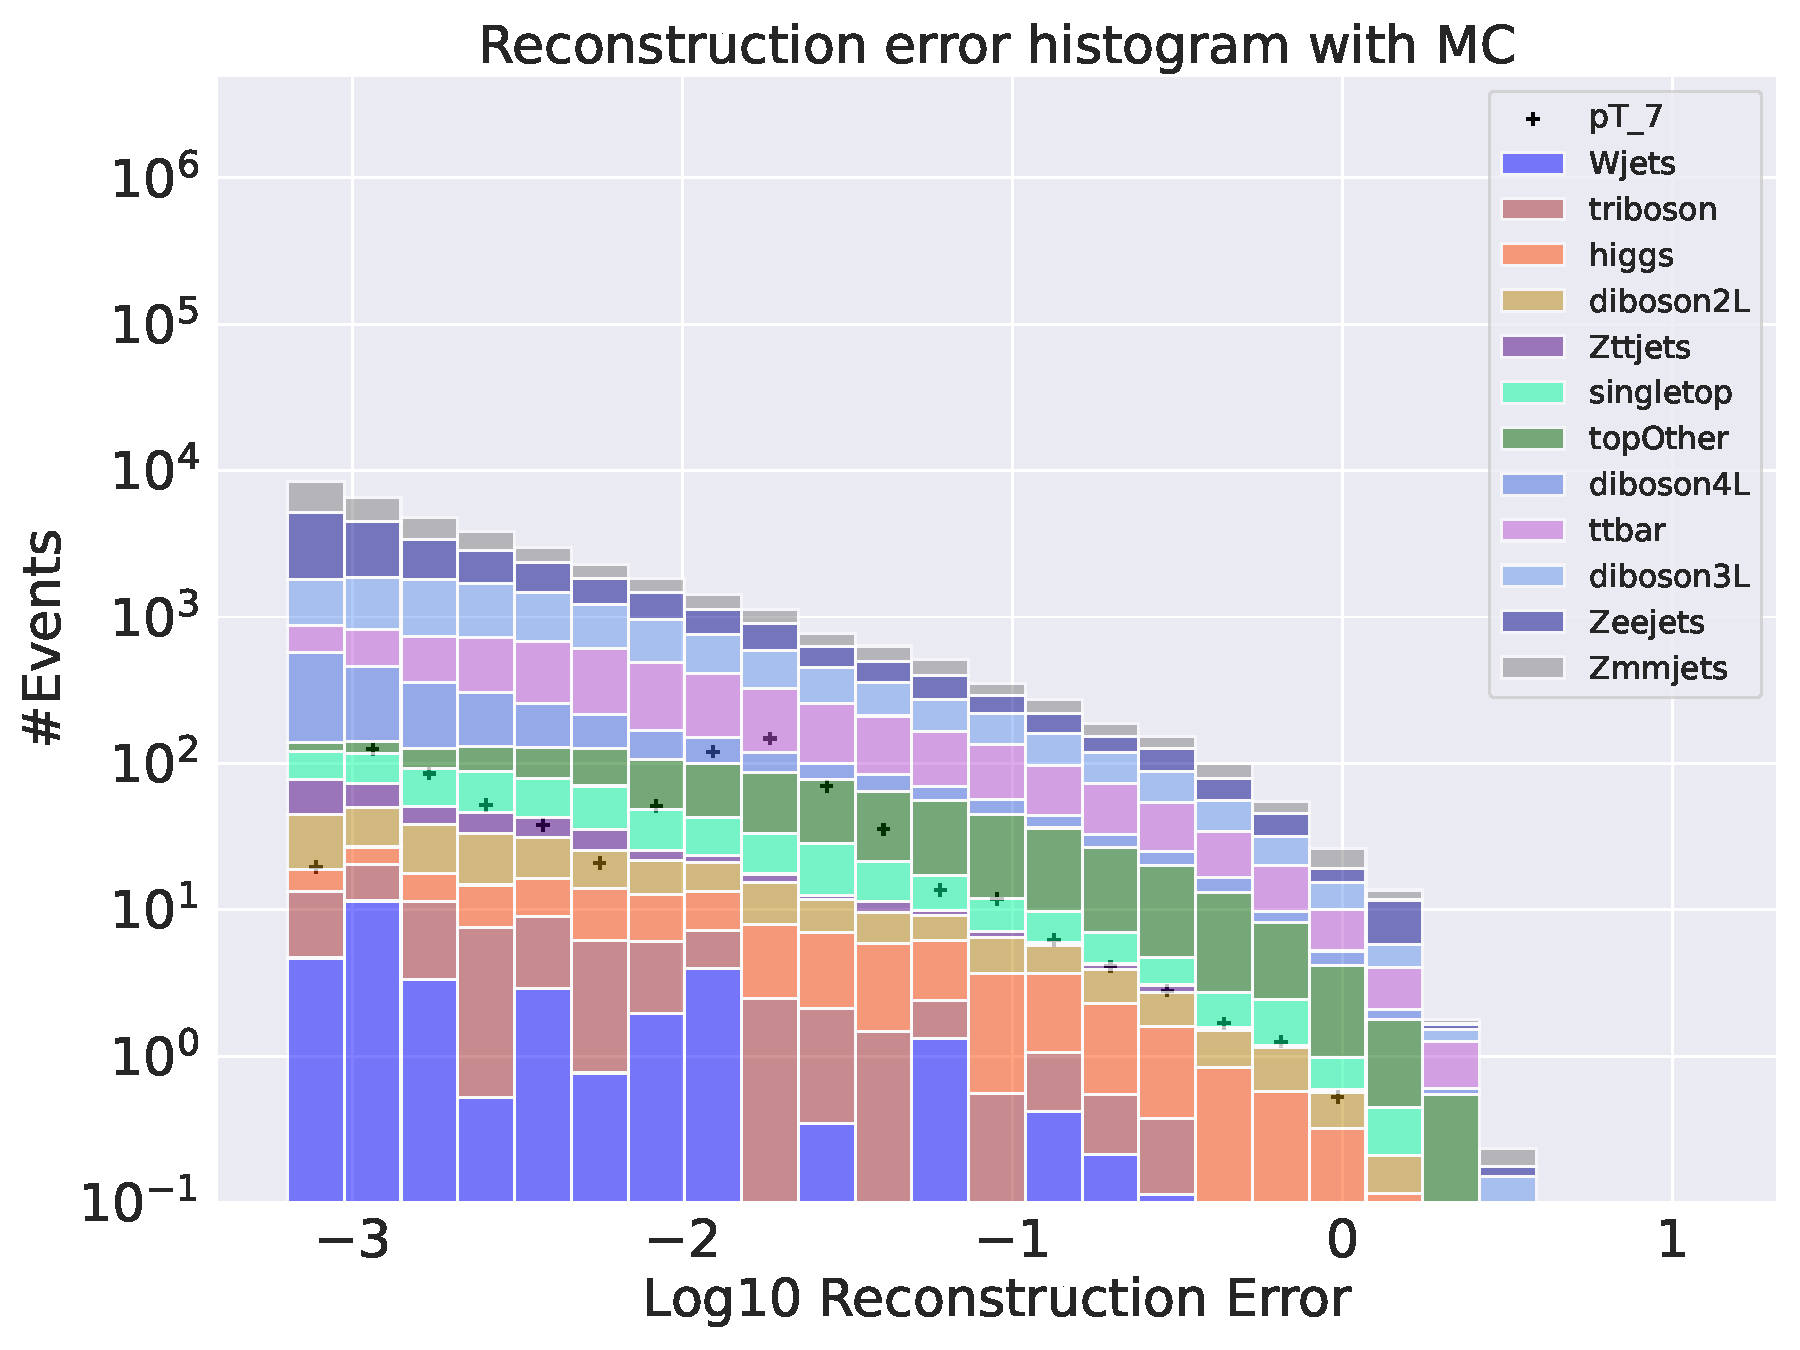
\includegraphics[width=\textwidth]{Figures/AE_testing/big/b_data_recon_big_rm3_feats_sig_pT_7.pdf}
        \caption{ }
        \label{fig:ae_big_pt_7}
    \end{subfigure}
    \hfill 
    \caption[AE | Reconstruction error $p_T$ altering of 7]{Reconstruction error on validation SM MC from the small (a) and large (b) regular Autoencoder. The signal is a subsample of the validation 
    set where the transverse momentum of the first electron and the first muon has been increased with a scale of $7$. The change of transverse 
    energy has also been changed according to the scaling of transverse momentum. No significant difference in distributions is found. }
    \label{fig:ae_big_small_pt_7}
\end{figure}

\begin{figure}[H]
    \centering
    \begin{subfigure}{.45\textwidth}
        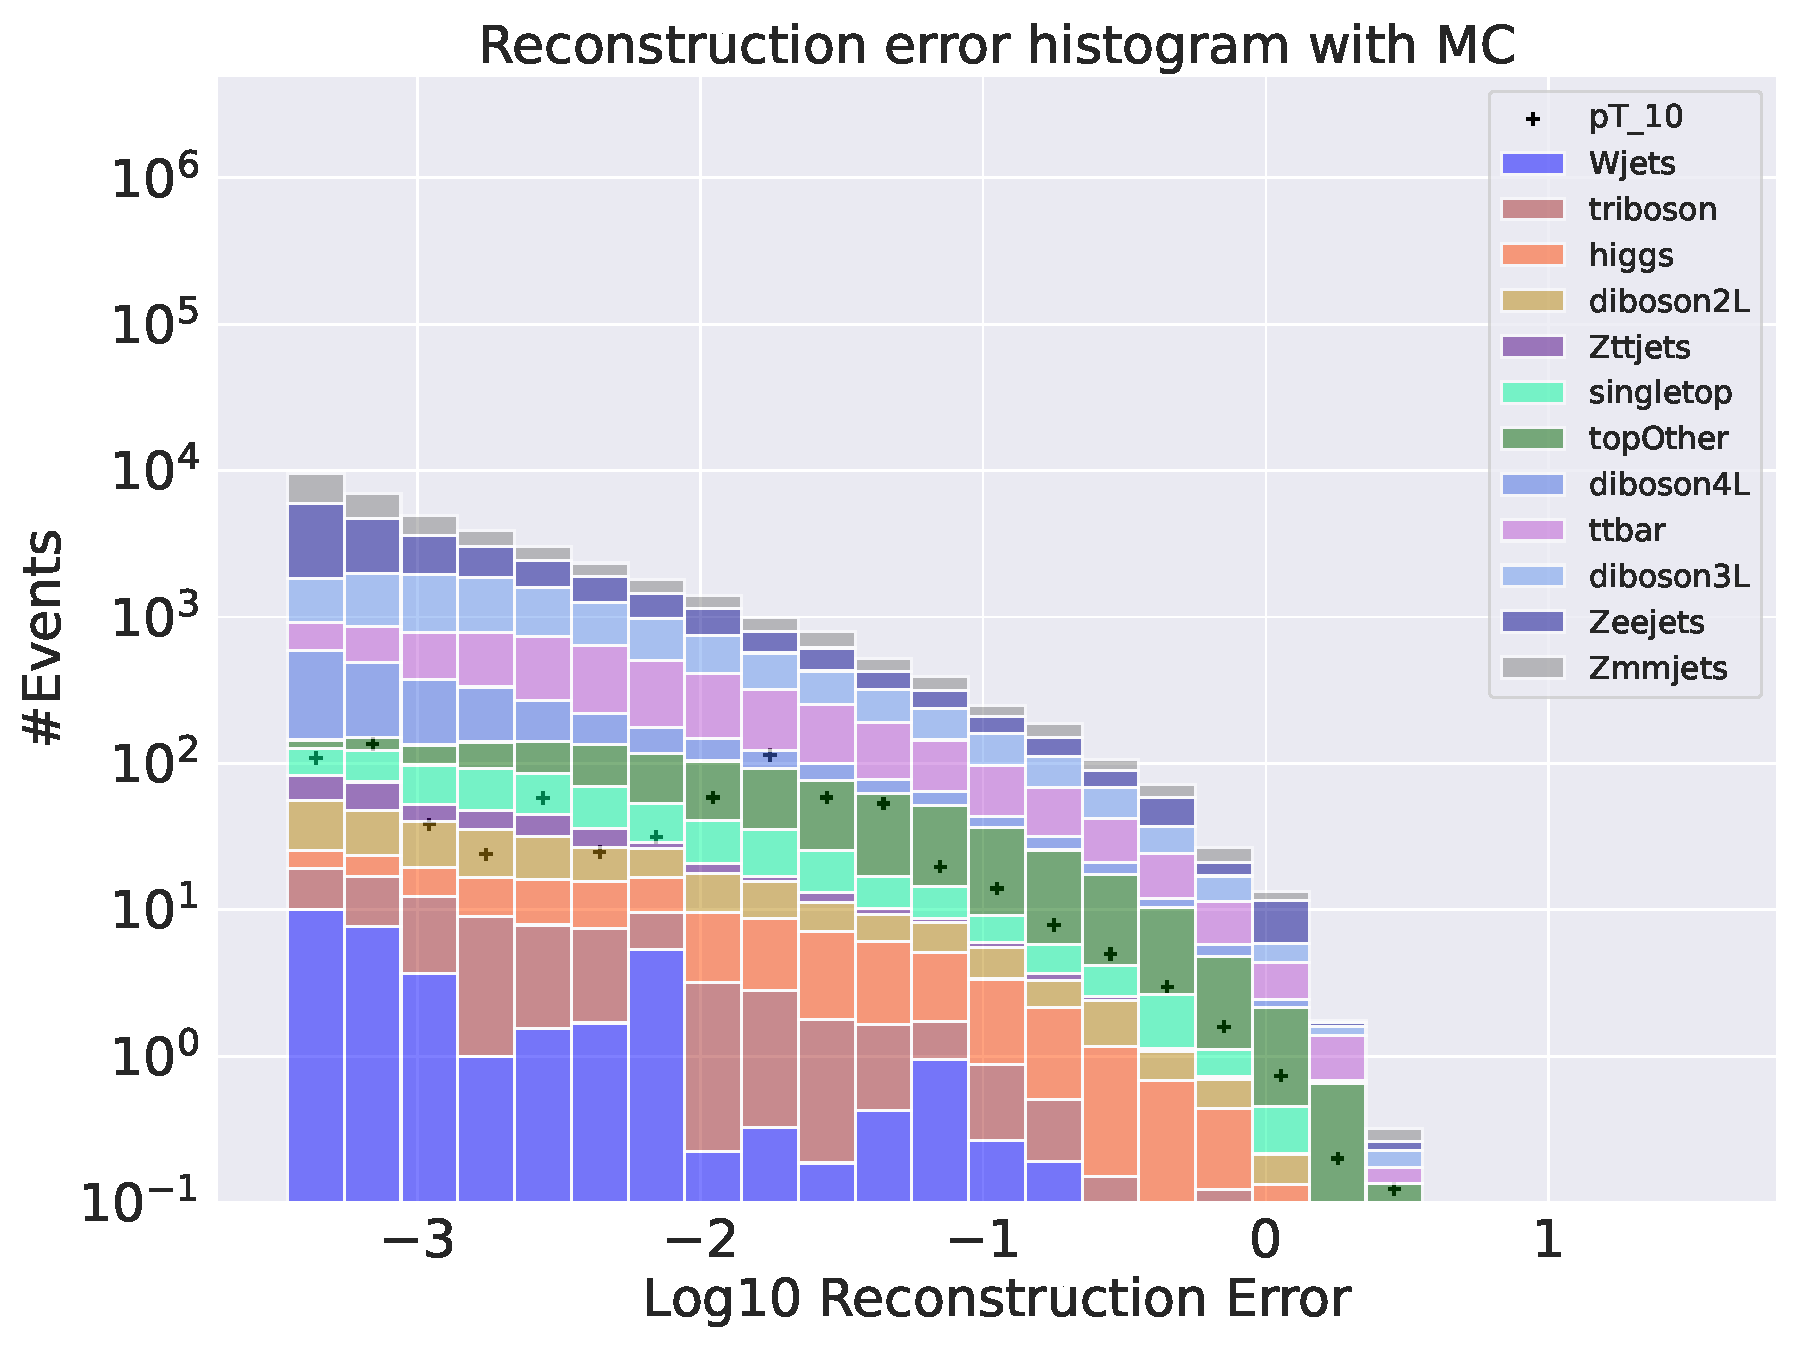
\includegraphics[width=\textwidth]{Figures/AE_testing/small/b_data_recon_big_rm3_feats_sig_pT_10.pdf}
        \caption{}
        \label{fig:ae_small_pt_10}
    \end{subfigure}
    \hfill 
    \begin{subfigure}{.45\textwidth}
        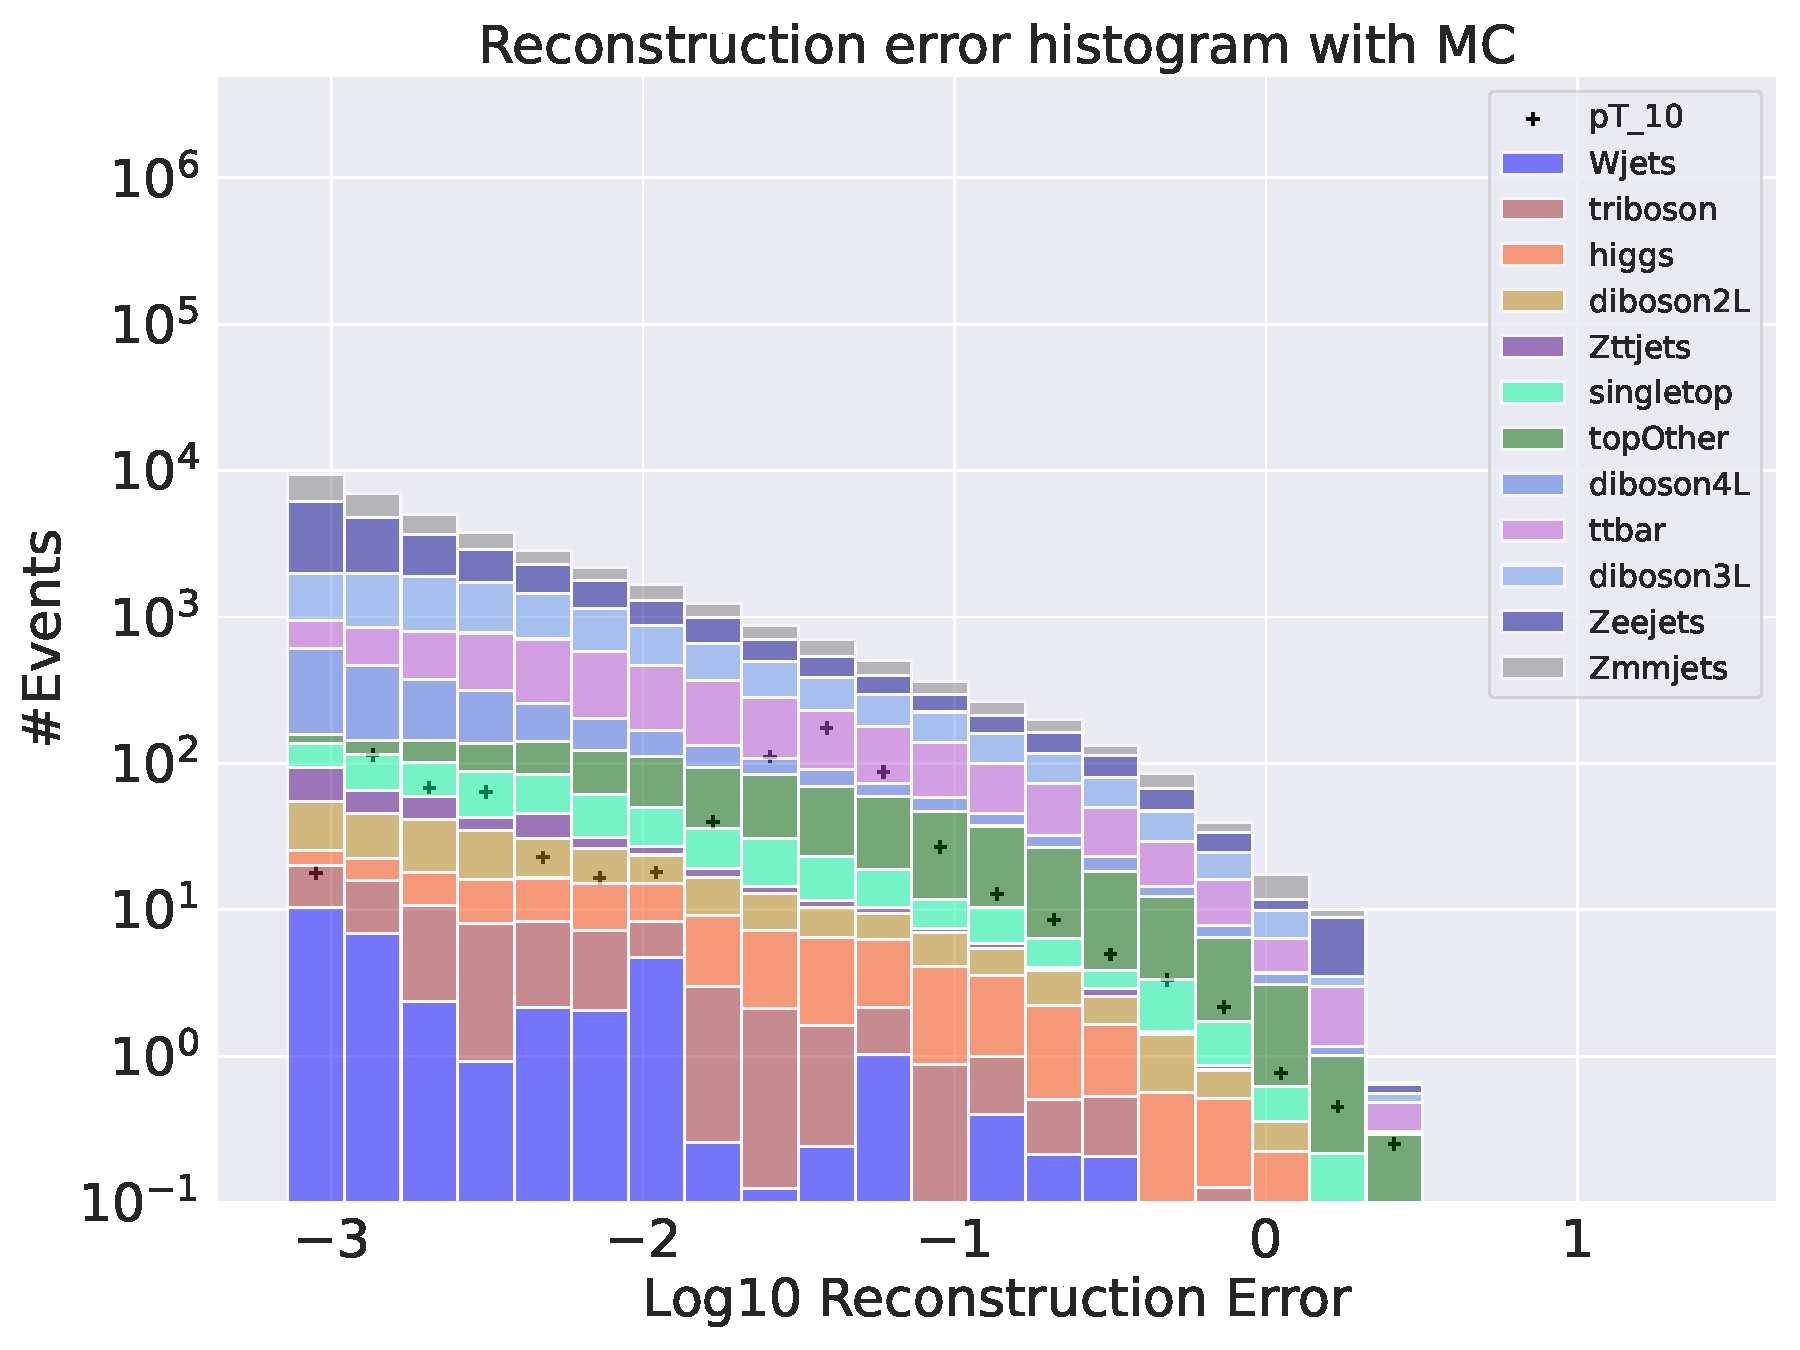
\includegraphics[width=\textwidth]{Figures/AE_testing/big/b_data_recon_big_rm3_feats_sig_pT_10.pdf}
        \caption{}
        \label{fig:ae_big_pt_10}
    \end{subfigure}
    \hfill 
    \caption[AE | Reconstruction error $p_T$ altering of 10]{Reconstruction error on validation SM MC from the small (a) and large (b) regular Autoencoder. The signal is a subsample of the validation 
    set where the transverse momentum of the first electron and the first muon has been increased with a scale of $10$. The change of transverse 
    energy has also been changed according to the scaling of transverse momentum. No significant difference in distributions is found. }
    \label{fig:ae_big_small_pt_10}
\end{figure}



\begin{figure}[H]
    \centering
    \begin{subfigure}{.45\textwidth}
        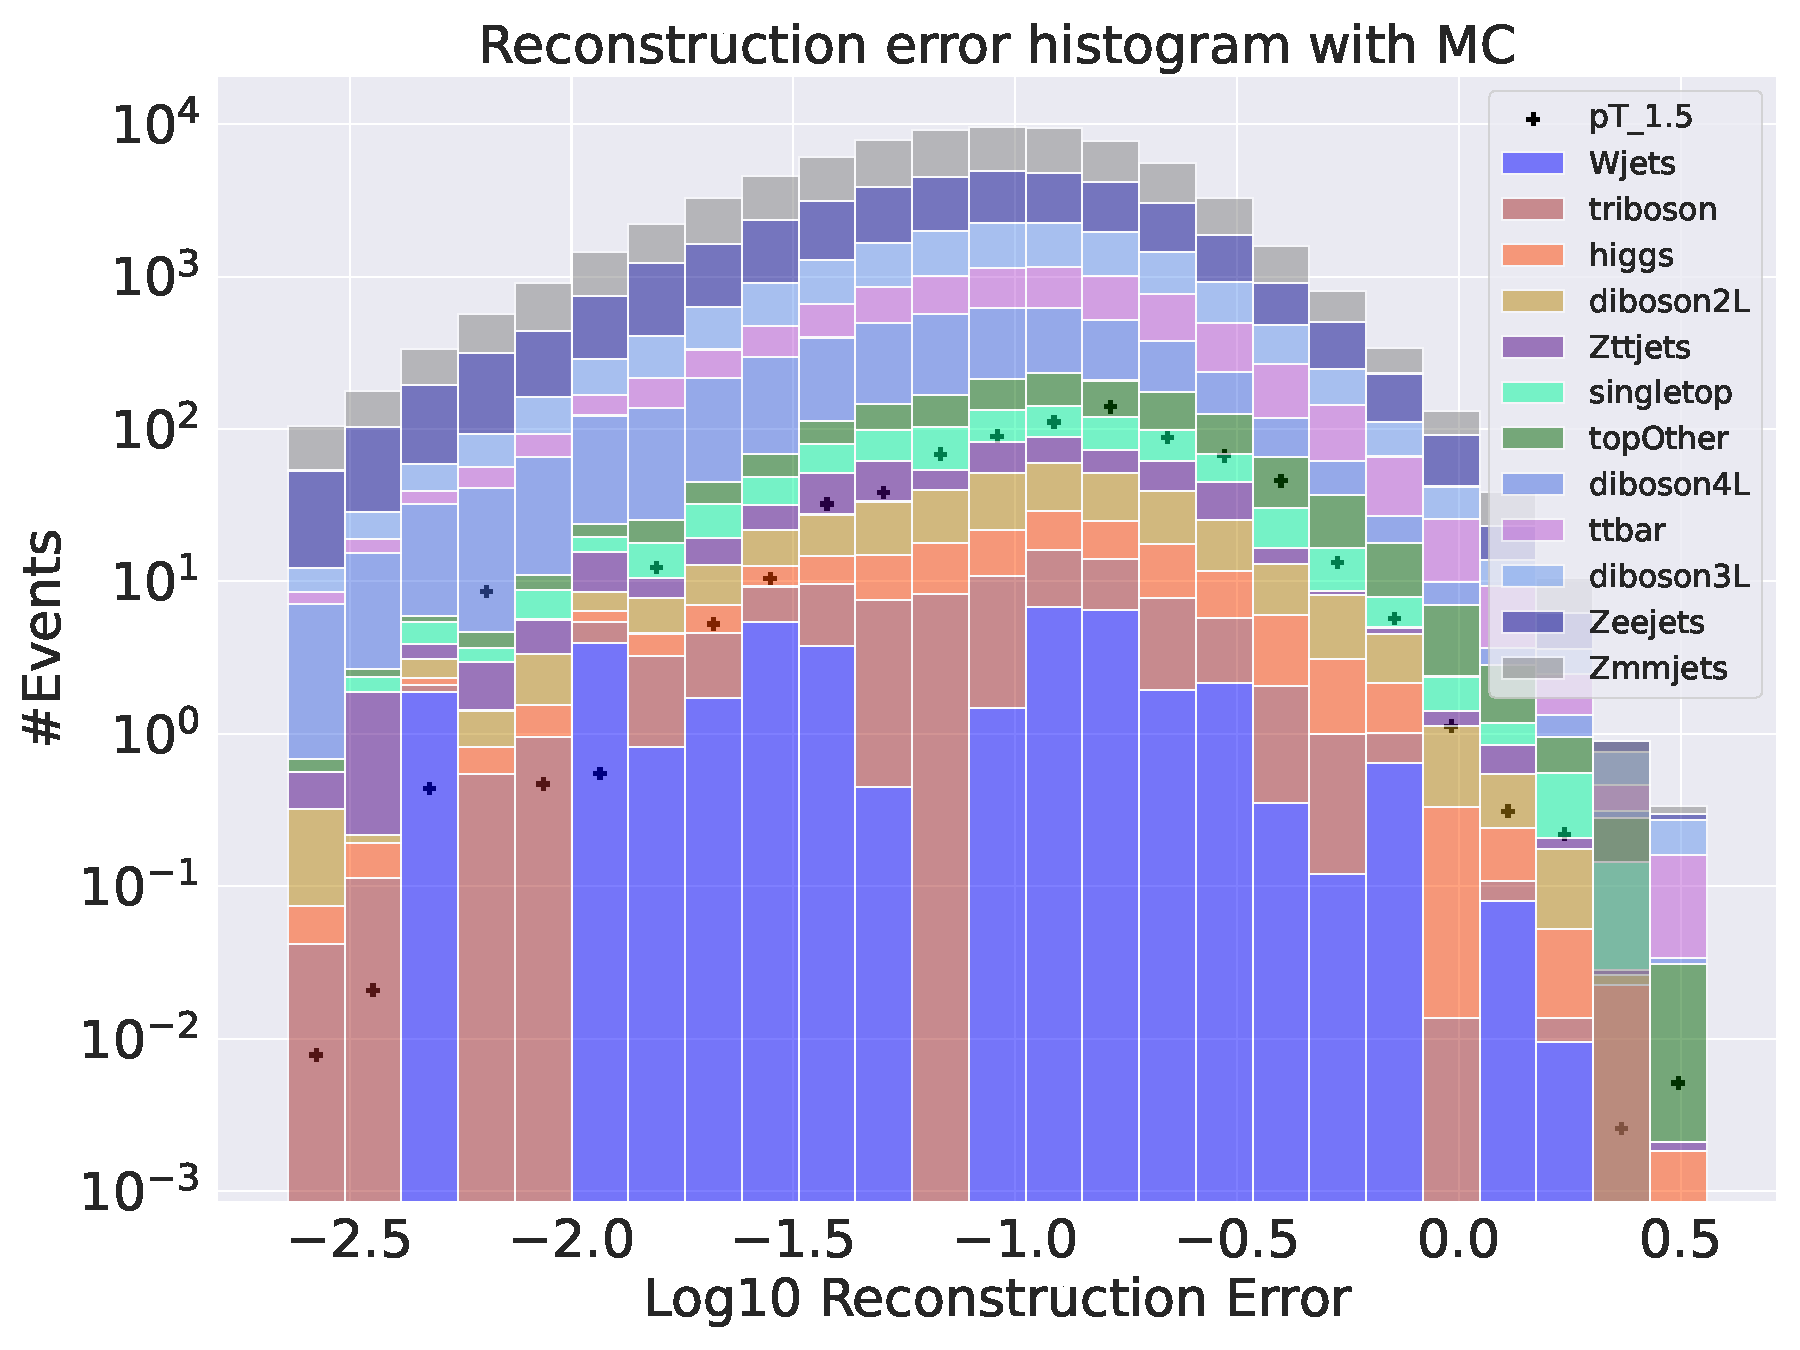
\includegraphics[width=\textwidth]{Figures/VAE_testing/small/b_data_recon_big_rm3_feats_sig_pT_1.5.pdf}
        \caption{}
        \label{fig:VAE_small_pt_1_5}
    \end{subfigure}
    \hfill 
    \begin{subfigure}{.45\textwidth}
        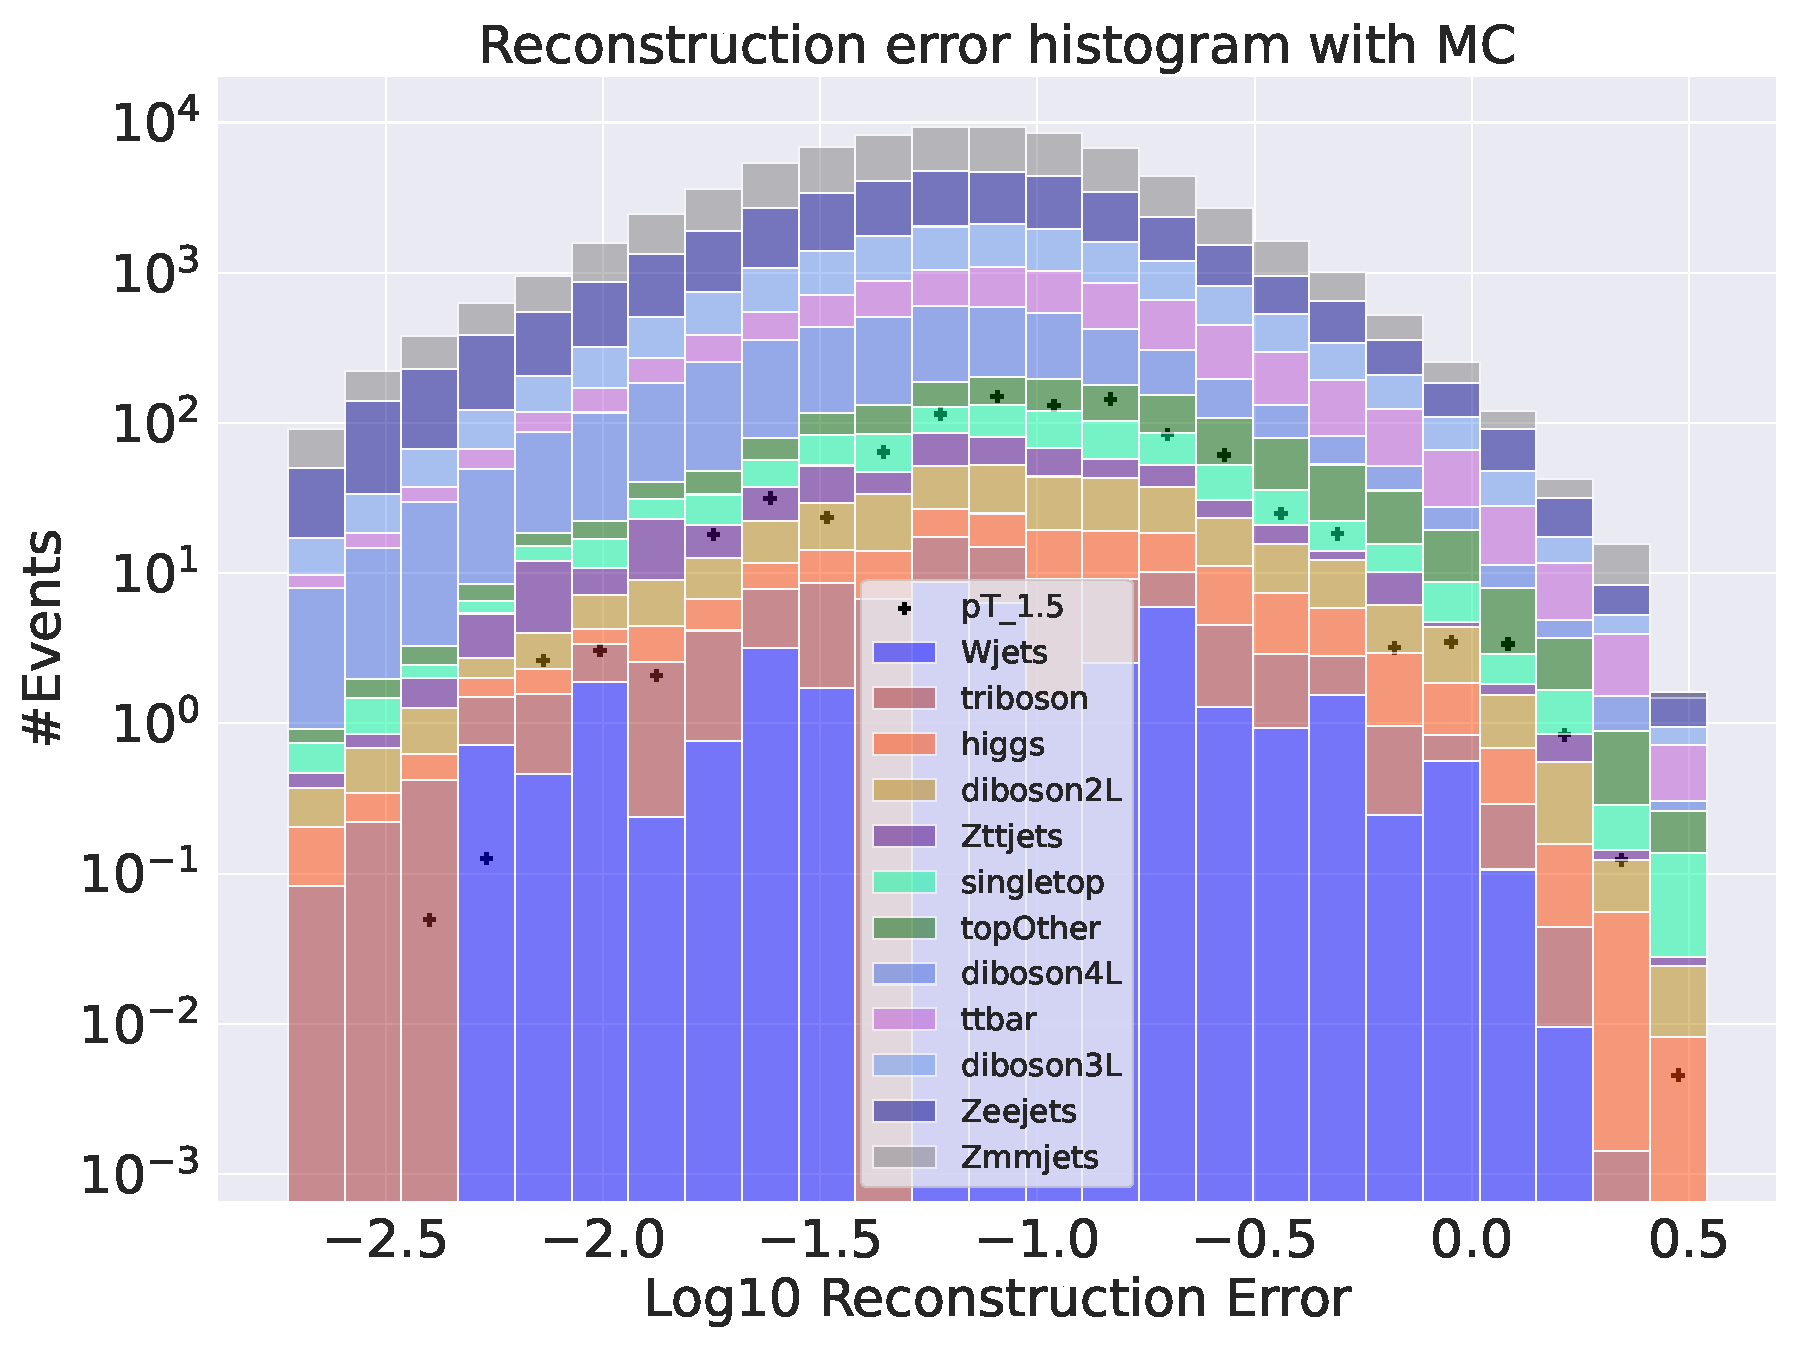
\includegraphics[width=\textwidth]{Figures/VAE_testing/big/b_data_recon_big_rm3_feats_sig_pT_1.5.pdf}
        \caption{ }
        \label{fig:VAE_big_pt_1_5}
    \end{subfigure}
    \hfill 
    \caption[VAE |Reconstruction error $p_T$ altering of 1.5]{Reconstruction error on validation SM MC from the small (a) and large (b) variational Autoencoder. The signal is a subsample of the validation 
    set where the transverse momentum of the first electron and the first muon has been increased with a scale of $1.5$. The change of transverse 
    energy has also been changed according to the scaling of transverse momentum. No significant difference in distributions is found. }
    \label{fig:VAE_big_small_pt_1_5}
\end{figure}

\begin{figure}[H]
    \centering
    \begin{subfigure}{.45\textwidth}
        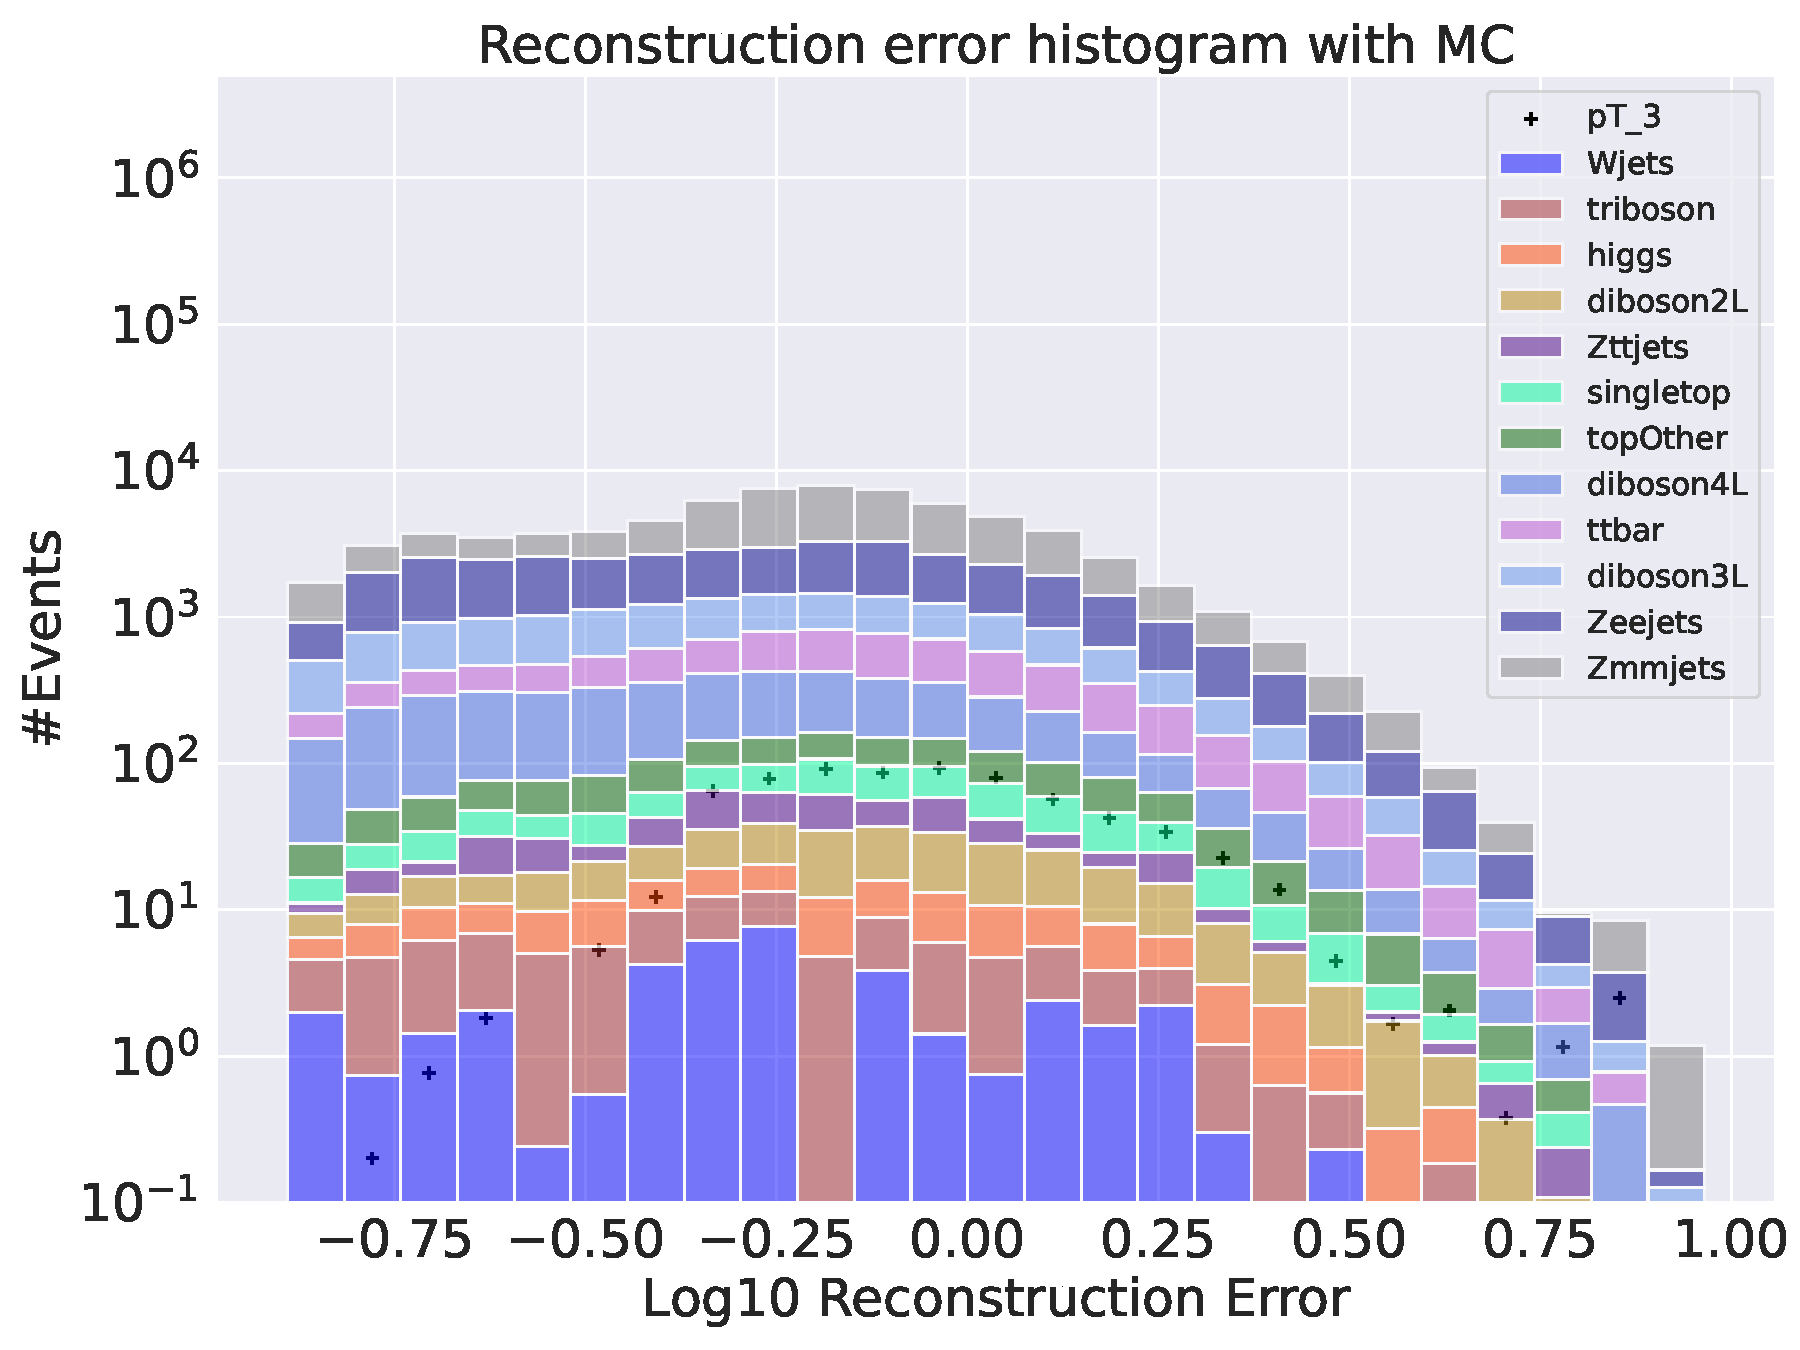
\includegraphics[width=\textwidth]{Figures/VAE_testing/small/b_data_recon_big_rm3_feats_sig_pT_3.pdf}
        \caption{ }
        \label{fig:VAE_small_pt_3}
    \end{subfigure}
    \hfill 
    \begin{subfigure}{.45\textwidth}
        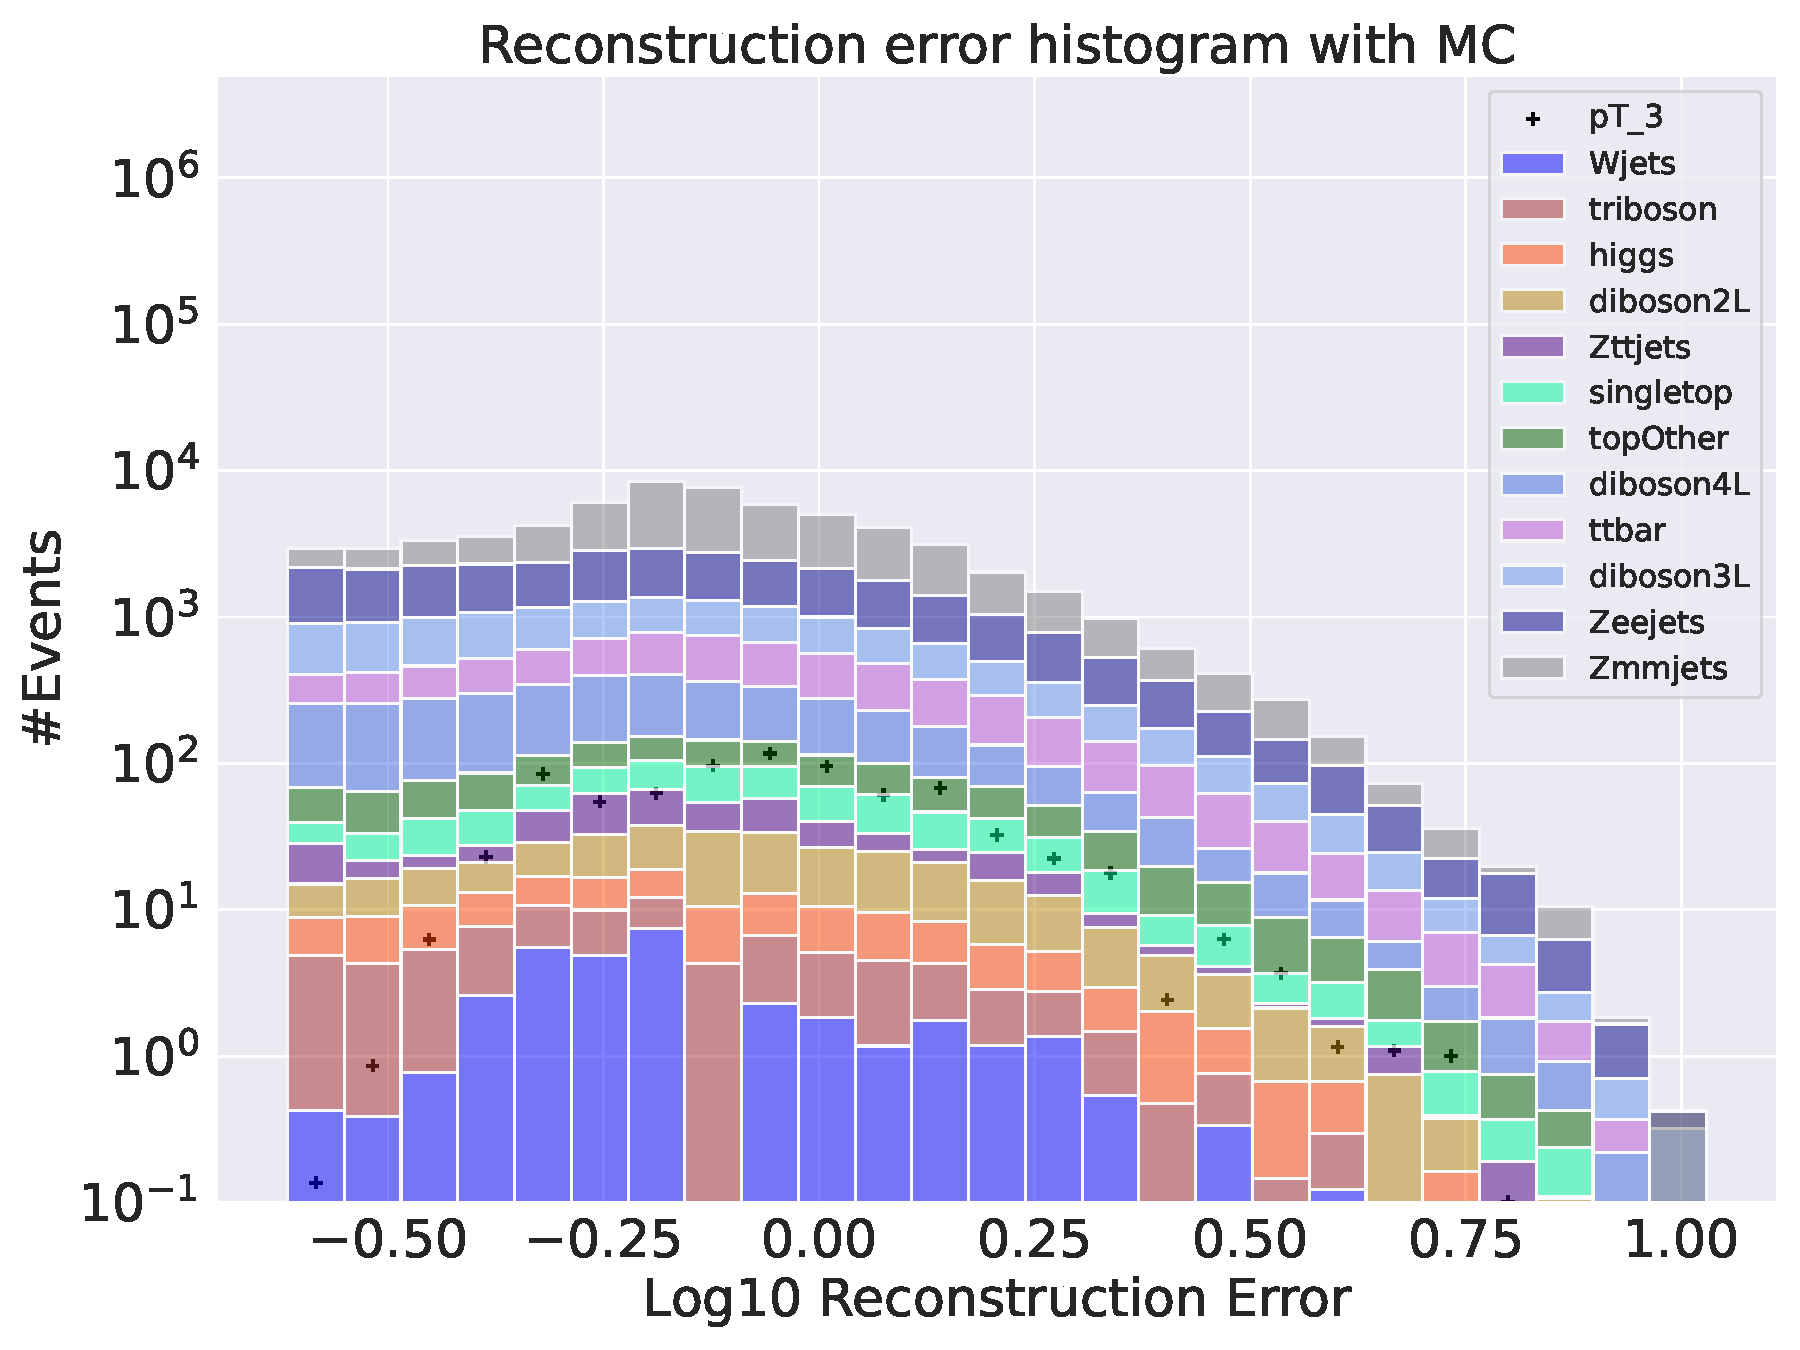
\includegraphics[width=\textwidth]{Figures/VAE_testing/big/b_data_recon_big_rm3_feats_sig_pT_3.pdf}
        \caption{ }
        \label{fig:VAE_big_pt_3}
    \end{subfigure}
    \hfill 
    \caption[VAE | Reconstruction error $p_T$ altering of 3]{Reconstruction error on validation SM MC from the small (a) and large (b) variational Autoencoder. The signal is a subsample of the validation 
    set where the transverse momentum of the first electron and the first muon has been increased with a scale of $3$. The change of transverse 
    energy has also been changed according to the scaling of transverse momentum. No significant difference in distributions is found.}
    \label{fig:VAE_big_small_pt_3}
\end{figure}

\begin{figure}[H]
    \centering
    \begin{subfigure}{.45\textwidth}
        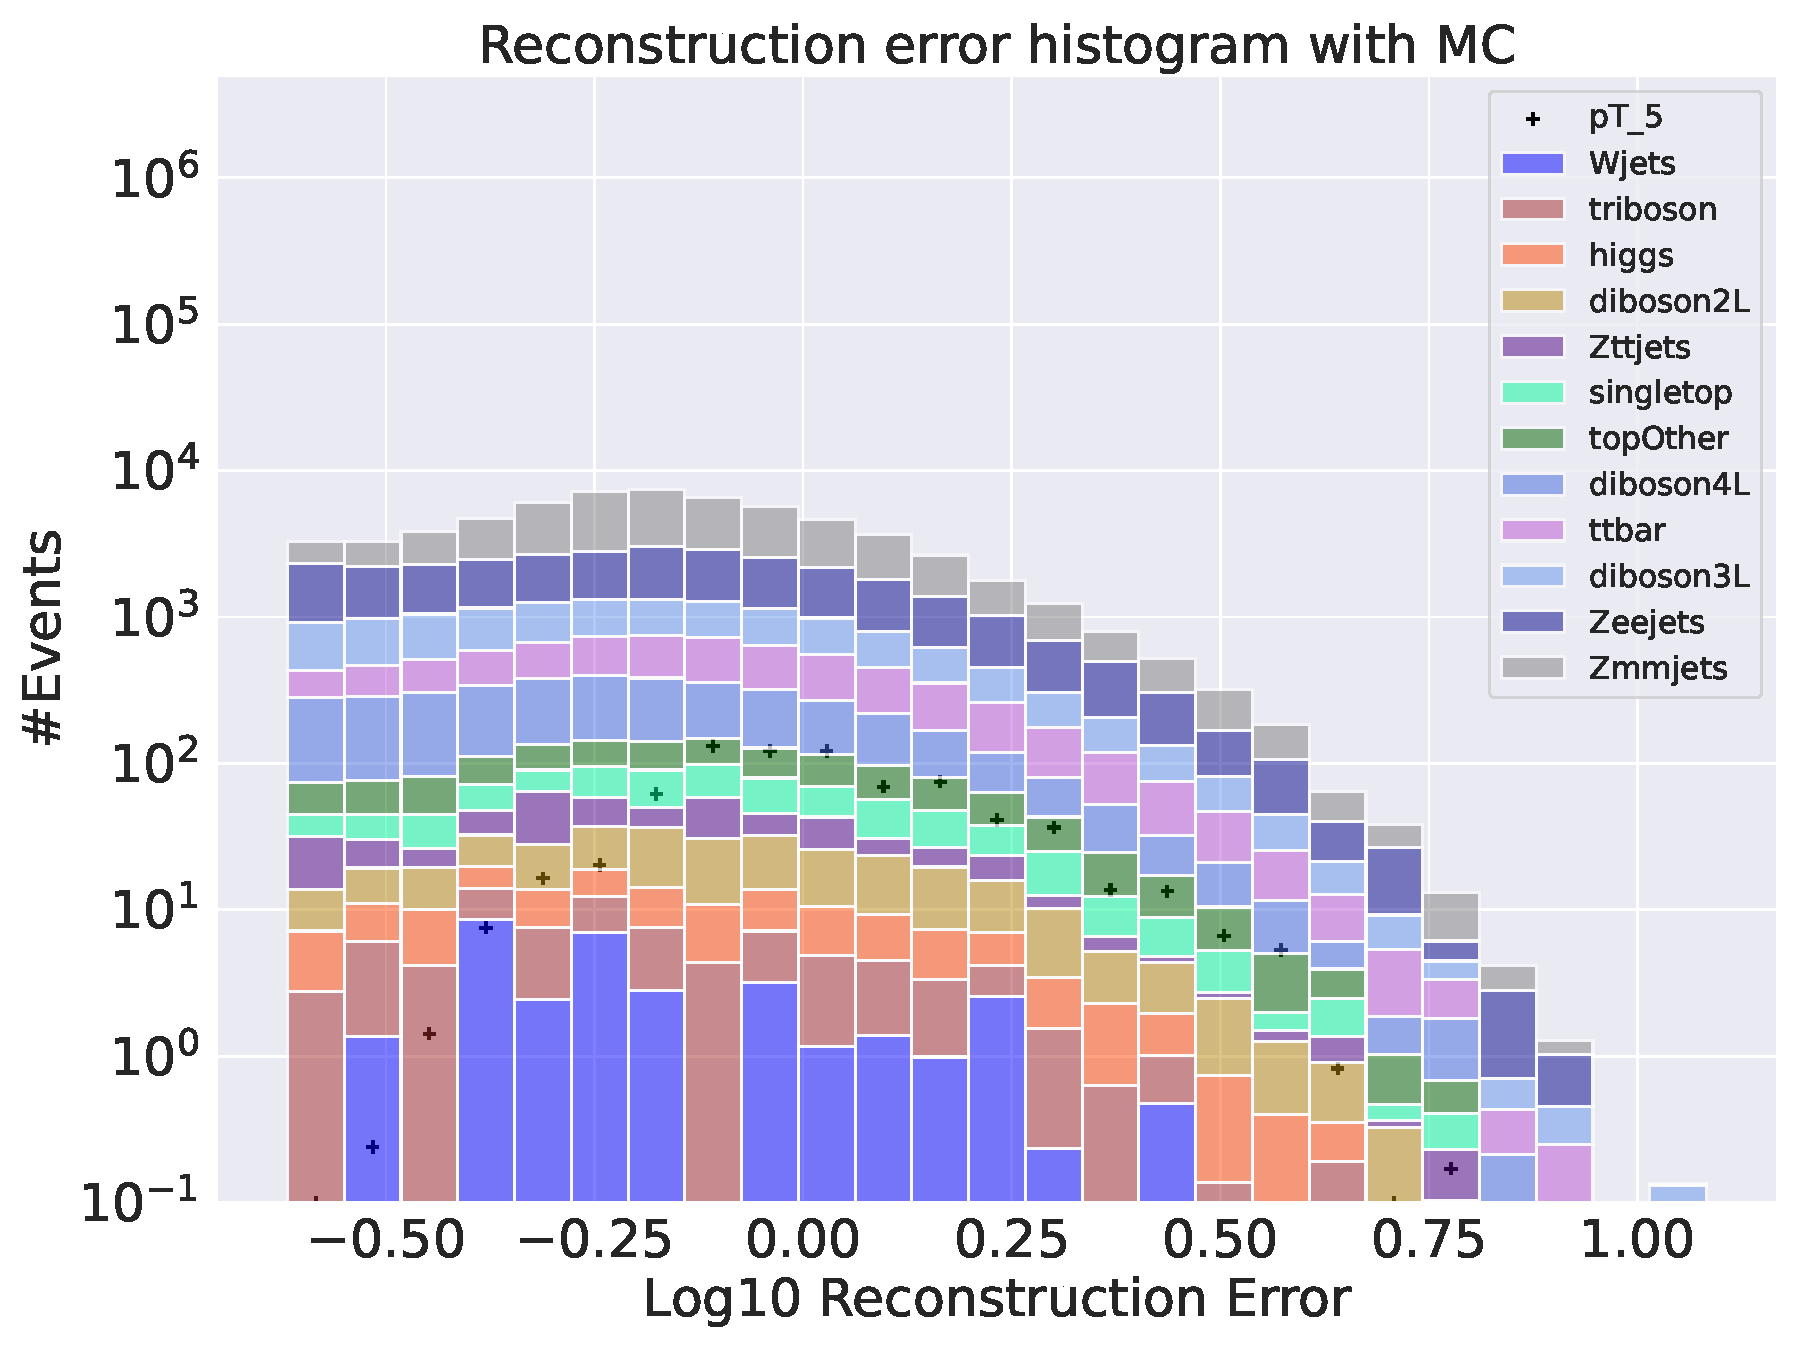
\includegraphics[width=\textwidth]{Figures/VAE_testing/small/b_data_recon_big_rm3_feats_sig_pT_5.pdf}
        \caption{}
        \label{fig:VAE_small_pt_5}
    \end{subfigure}
    \hfill 
    \begin{subfigure}{.45\textwidth}
        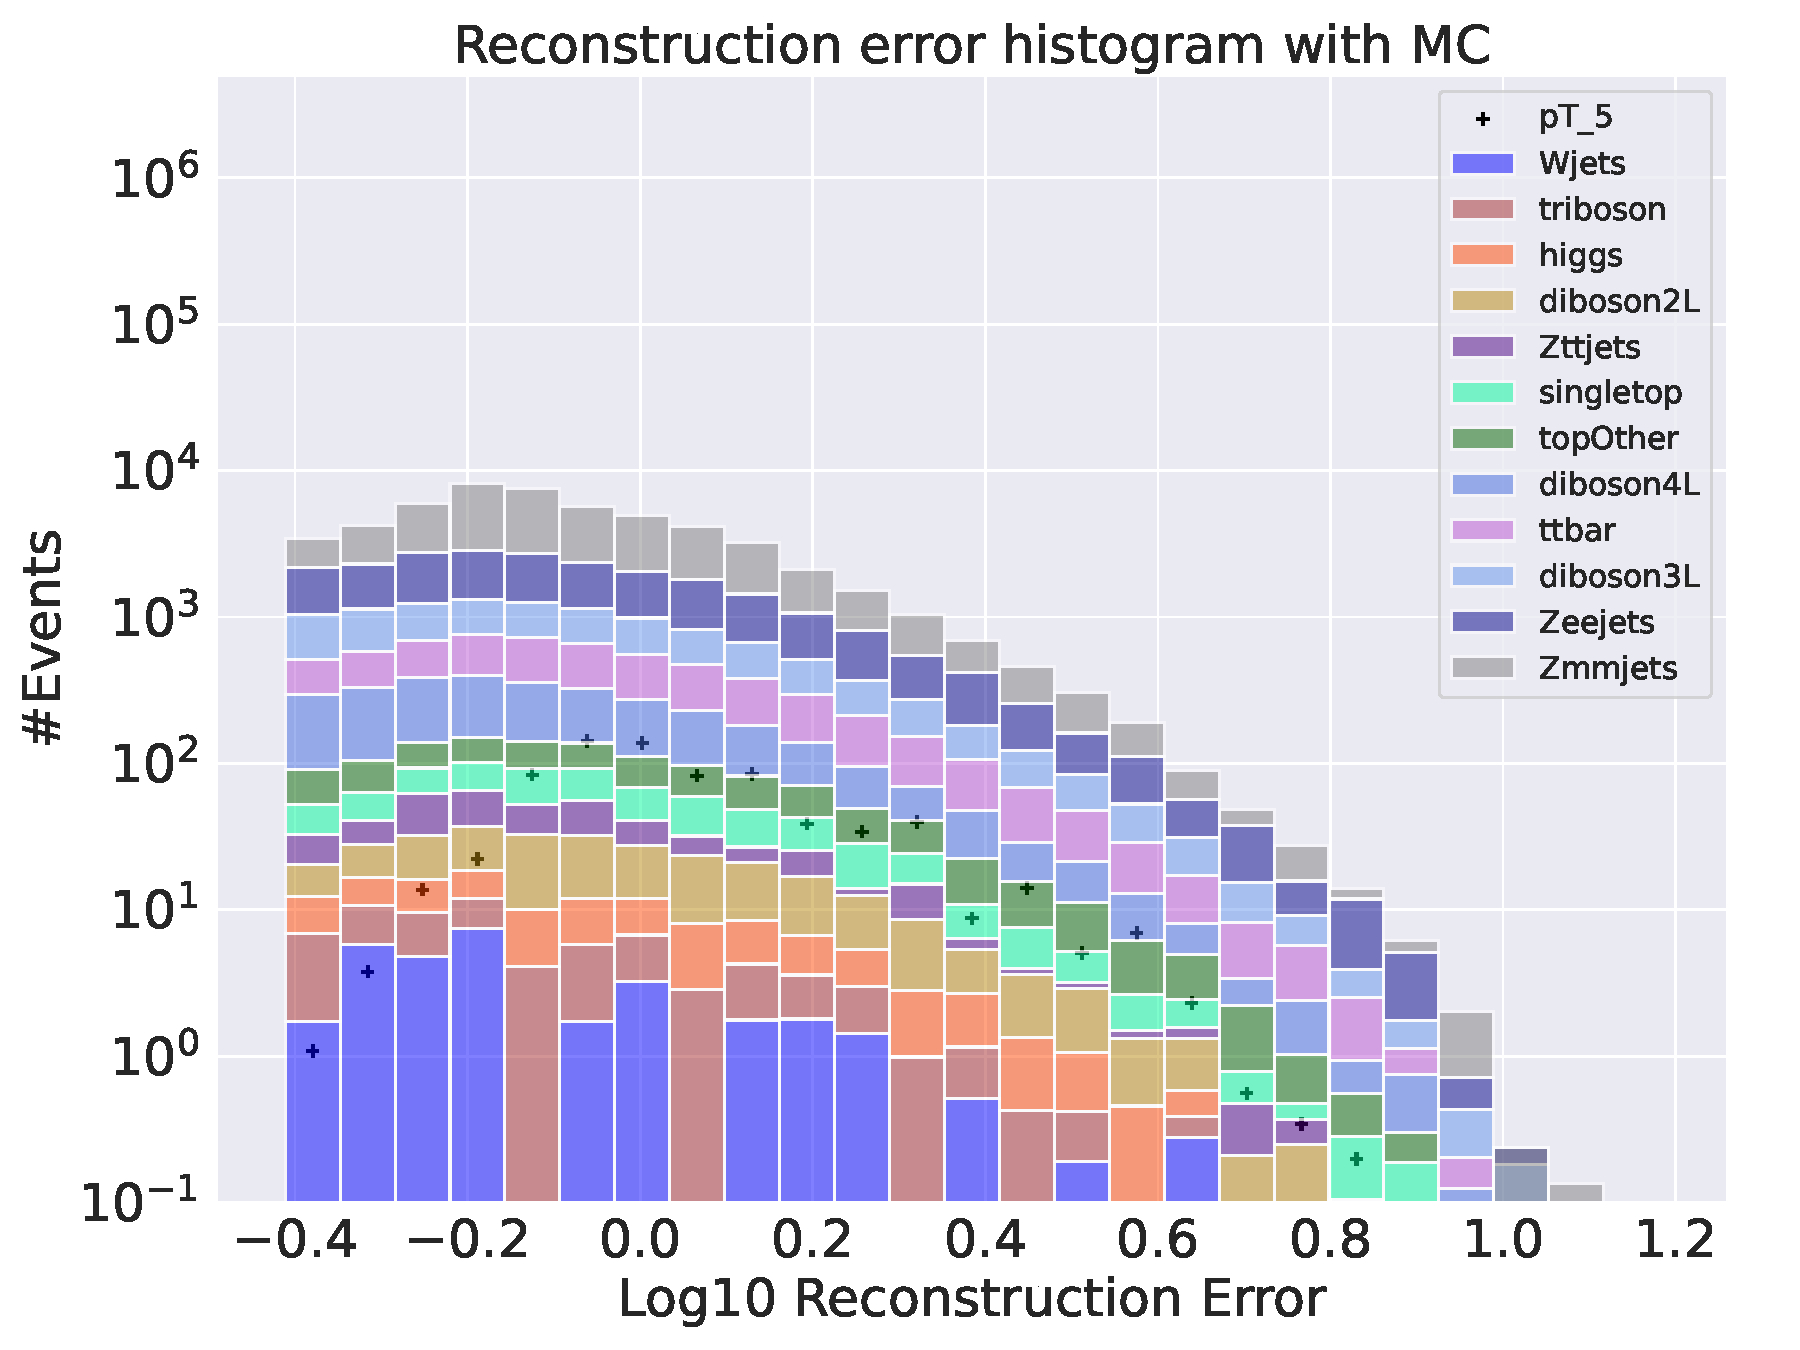
\includegraphics[width=\textwidth]{Figures/VAE_testing/big/b_data_recon_big_rm3_feats_sig_pT_5.pdf}
        \caption{ }
        \label{fig:VAE_big_pt_5}
    \end{subfigure}
    \hfill 
    \caption[VAE | Reconstruction error $p_T$ altering of 5]{Reconstruction error on validation SM MC from the small (a) and large (b) variational Autoencoder.The signal is a subsample of the validation 
    set where the transverse momentum of the first electron and the first muon has been increased with a scale of $5$. The change of transverse 
    energy has also been changed according to the scaling of transverse momentum.  No significant difference in distributions is found.  }
    \label{fig:VAE_big_small_pt_5}
\end{figure}


\begin{figure}[H]
    \centering
    \begin{subfigure}{.45\textwidth}
        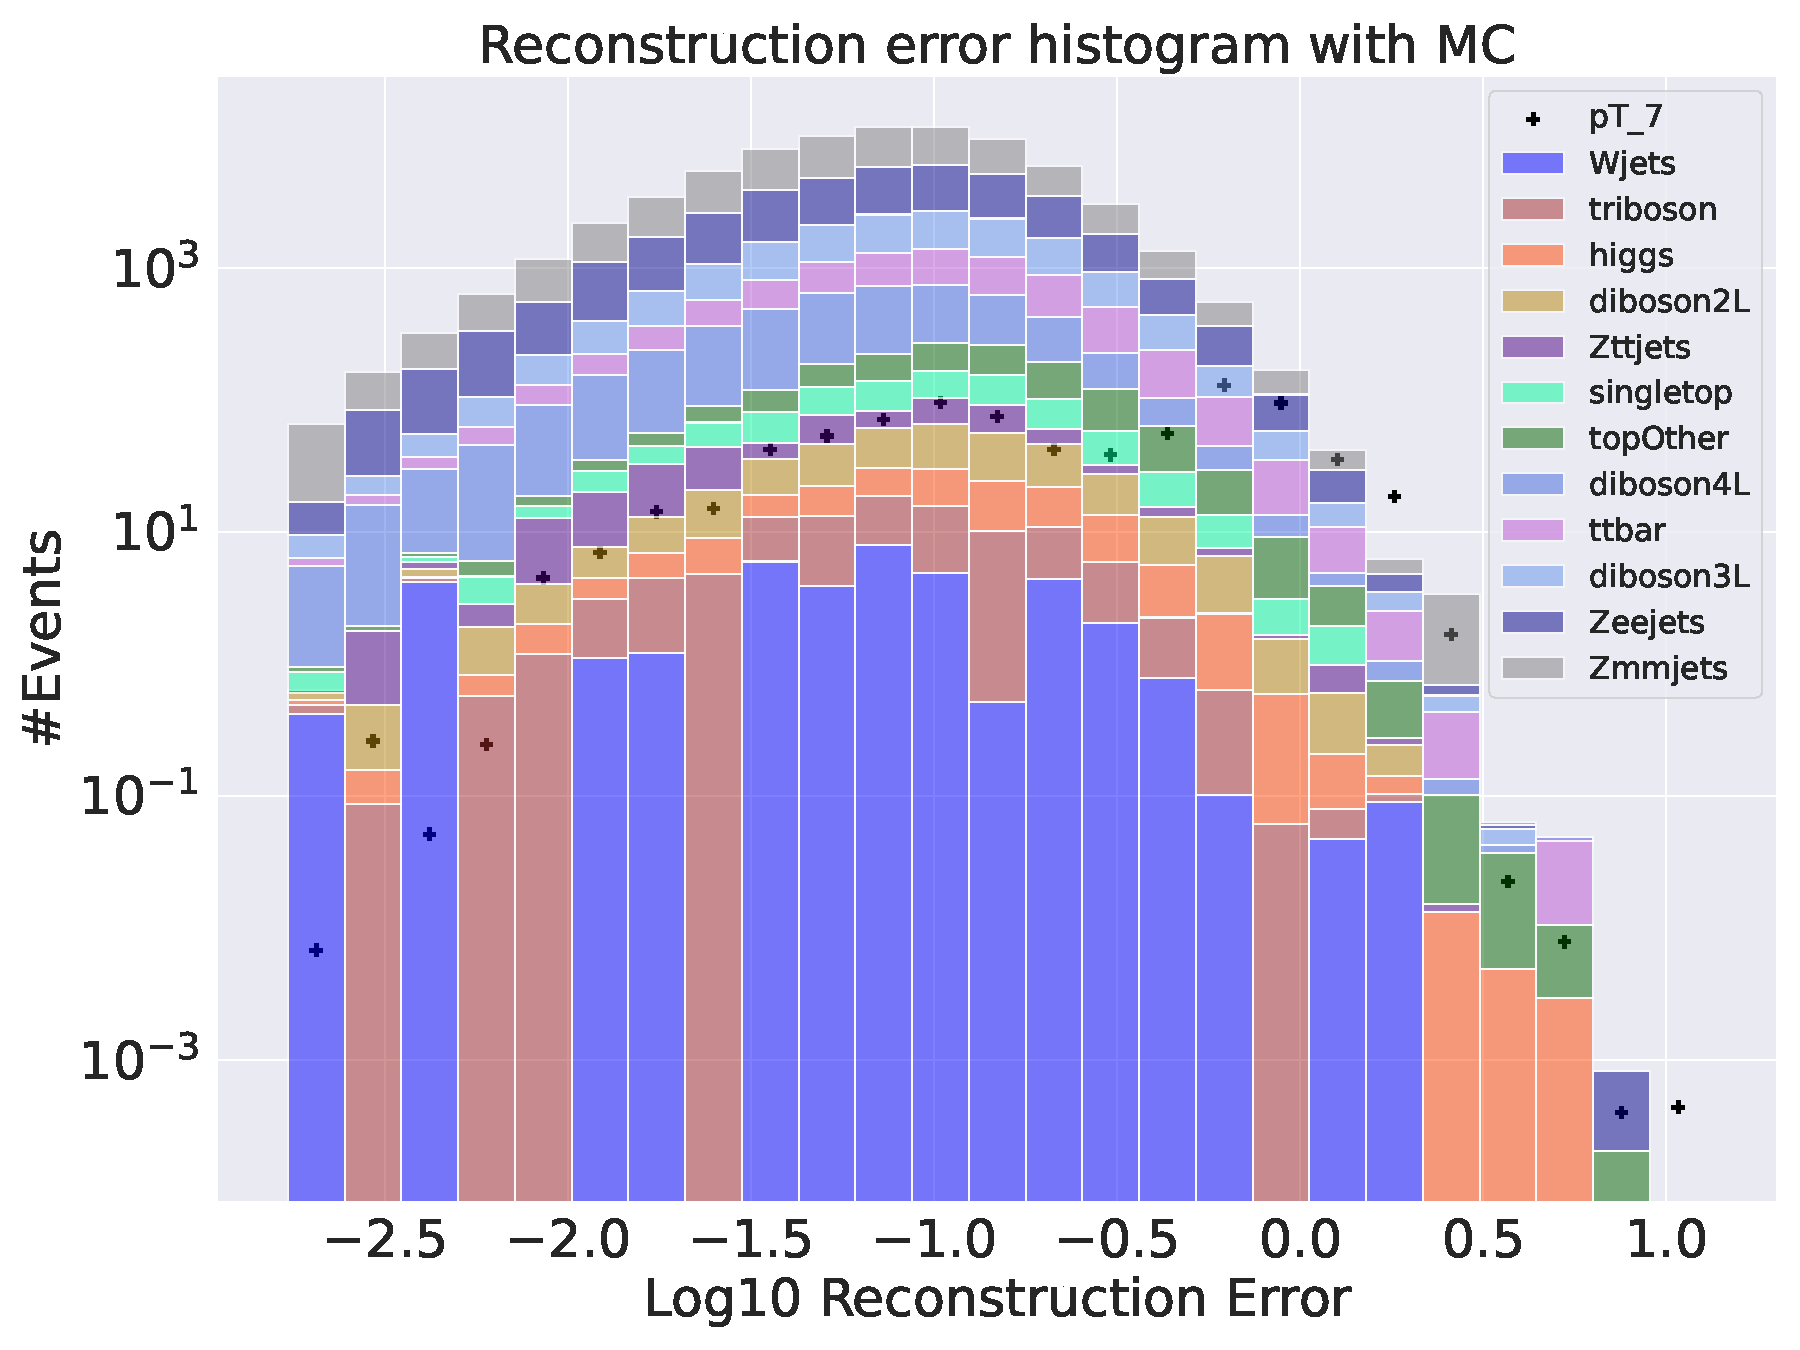
\includegraphics[width=\textwidth]{Figures/VAE_testing/small/b_data_recon_big_rm3_feats_sig_pT_7.pdf}
        \caption{}
        \label{fig:VAE_small_pt_7}
    \end{subfigure}
    \hfill 
    \begin{subfigure}{.45\textwidth}
        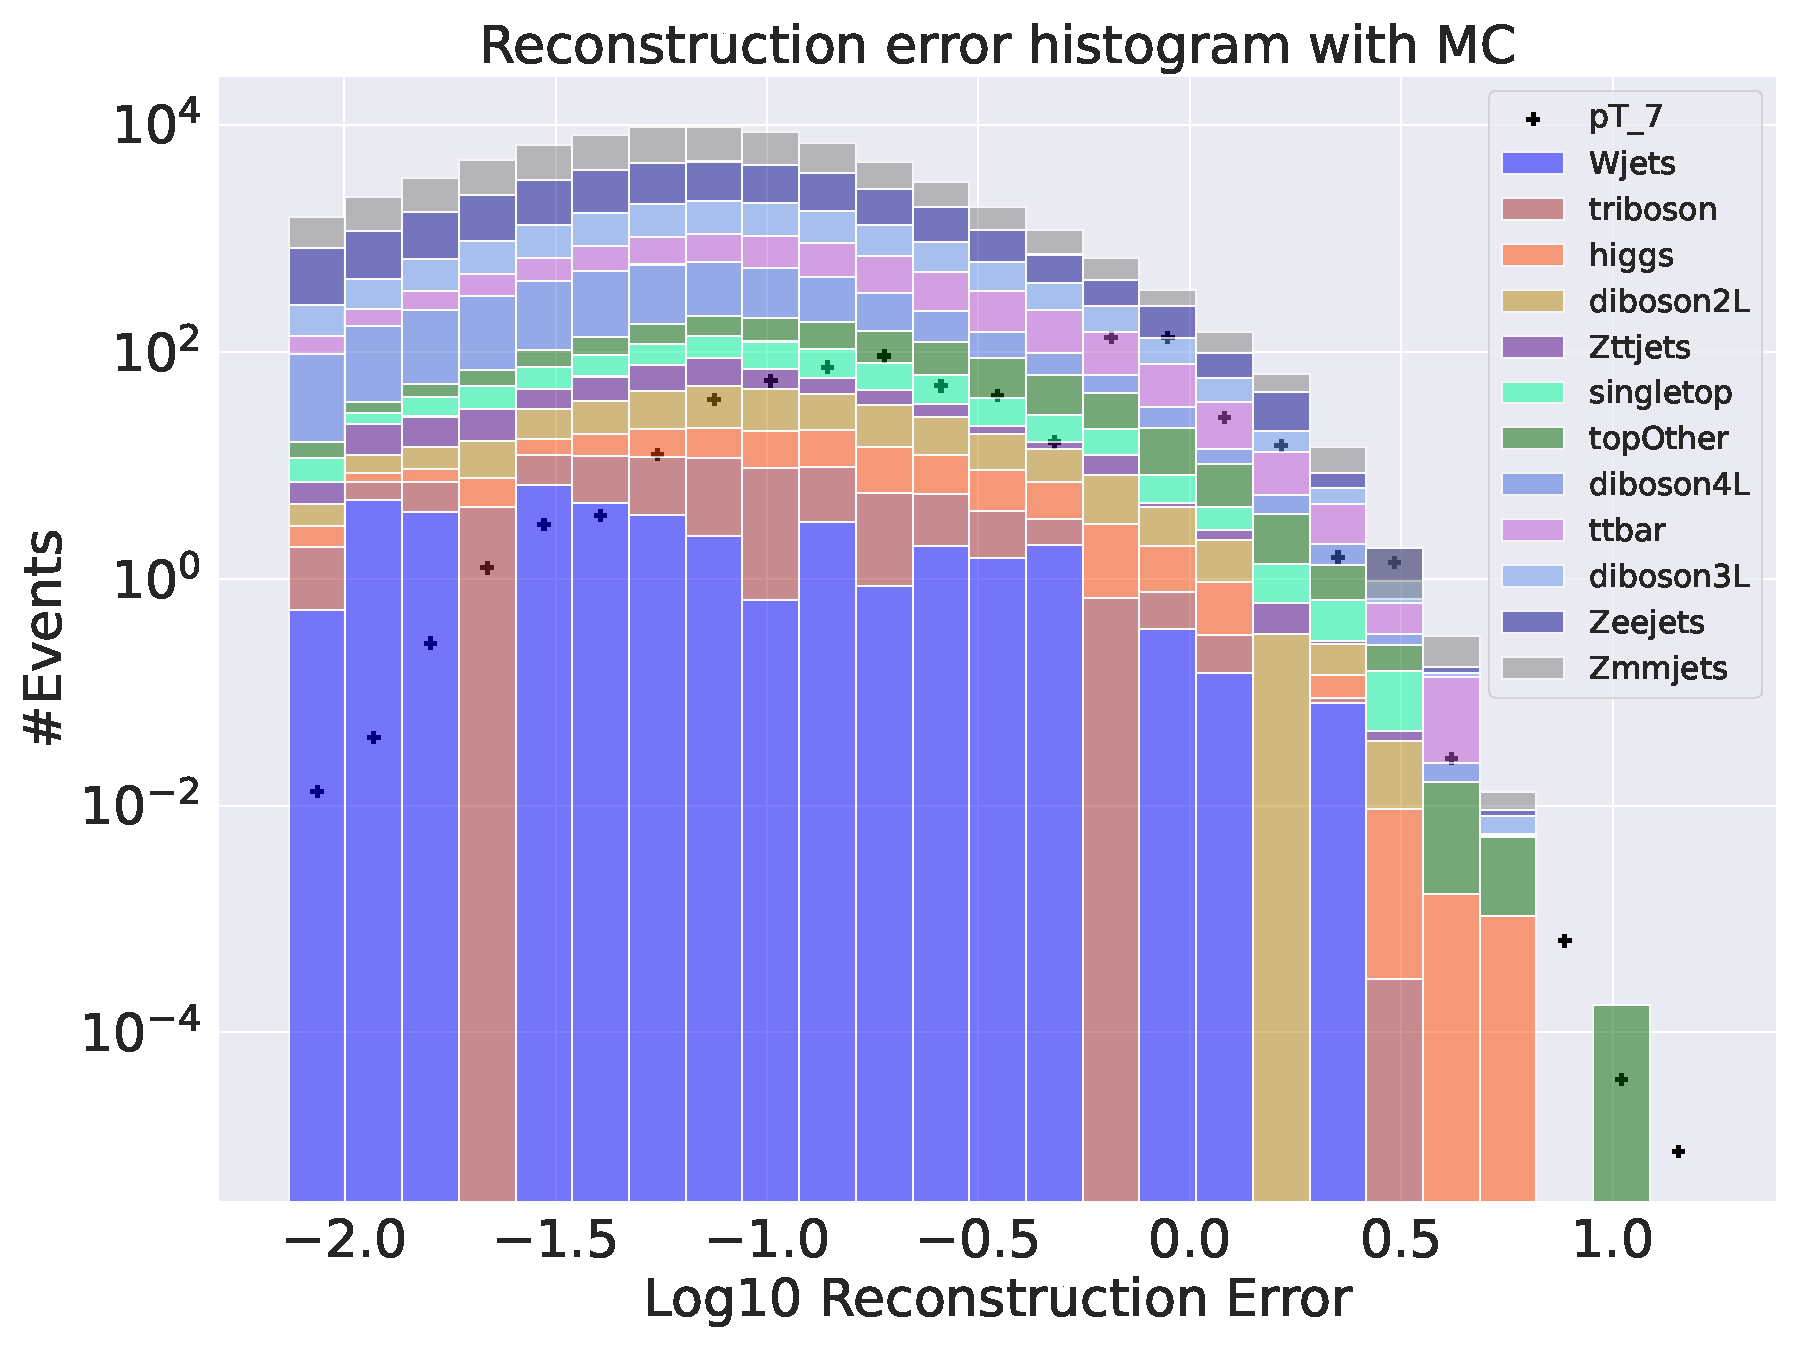
\includegraphics[width=\textwidth]{Figures/VAE_testing/big/b_data_recon_big_rm3_feats_sig_pT_7.pdf}
        \caption{ }
        \label{fig:VAE_big_pt_7}
    \end{subfigure}
    \hfill 
    \caption[VAE | Reconstruction error $p_T$ altering of 7]{Reconstruction error on validation SM MC from the small (a) and large (b) variational Autoencoder. The signal is a subsample of the validation 
    set where the transverse momentum of the first electron and the first muon has been increased with a scale of $7$. The change of transverse 
    energy has also been changed according to the scaling of transverse momentum. No significant difference in distributions is found.  }
    \label{fig:VAE_big_small_pt_7}
\end{figure}

\begin{figure}[H]
    \centering
    \begin{subfigure}{.45\textwidth}
        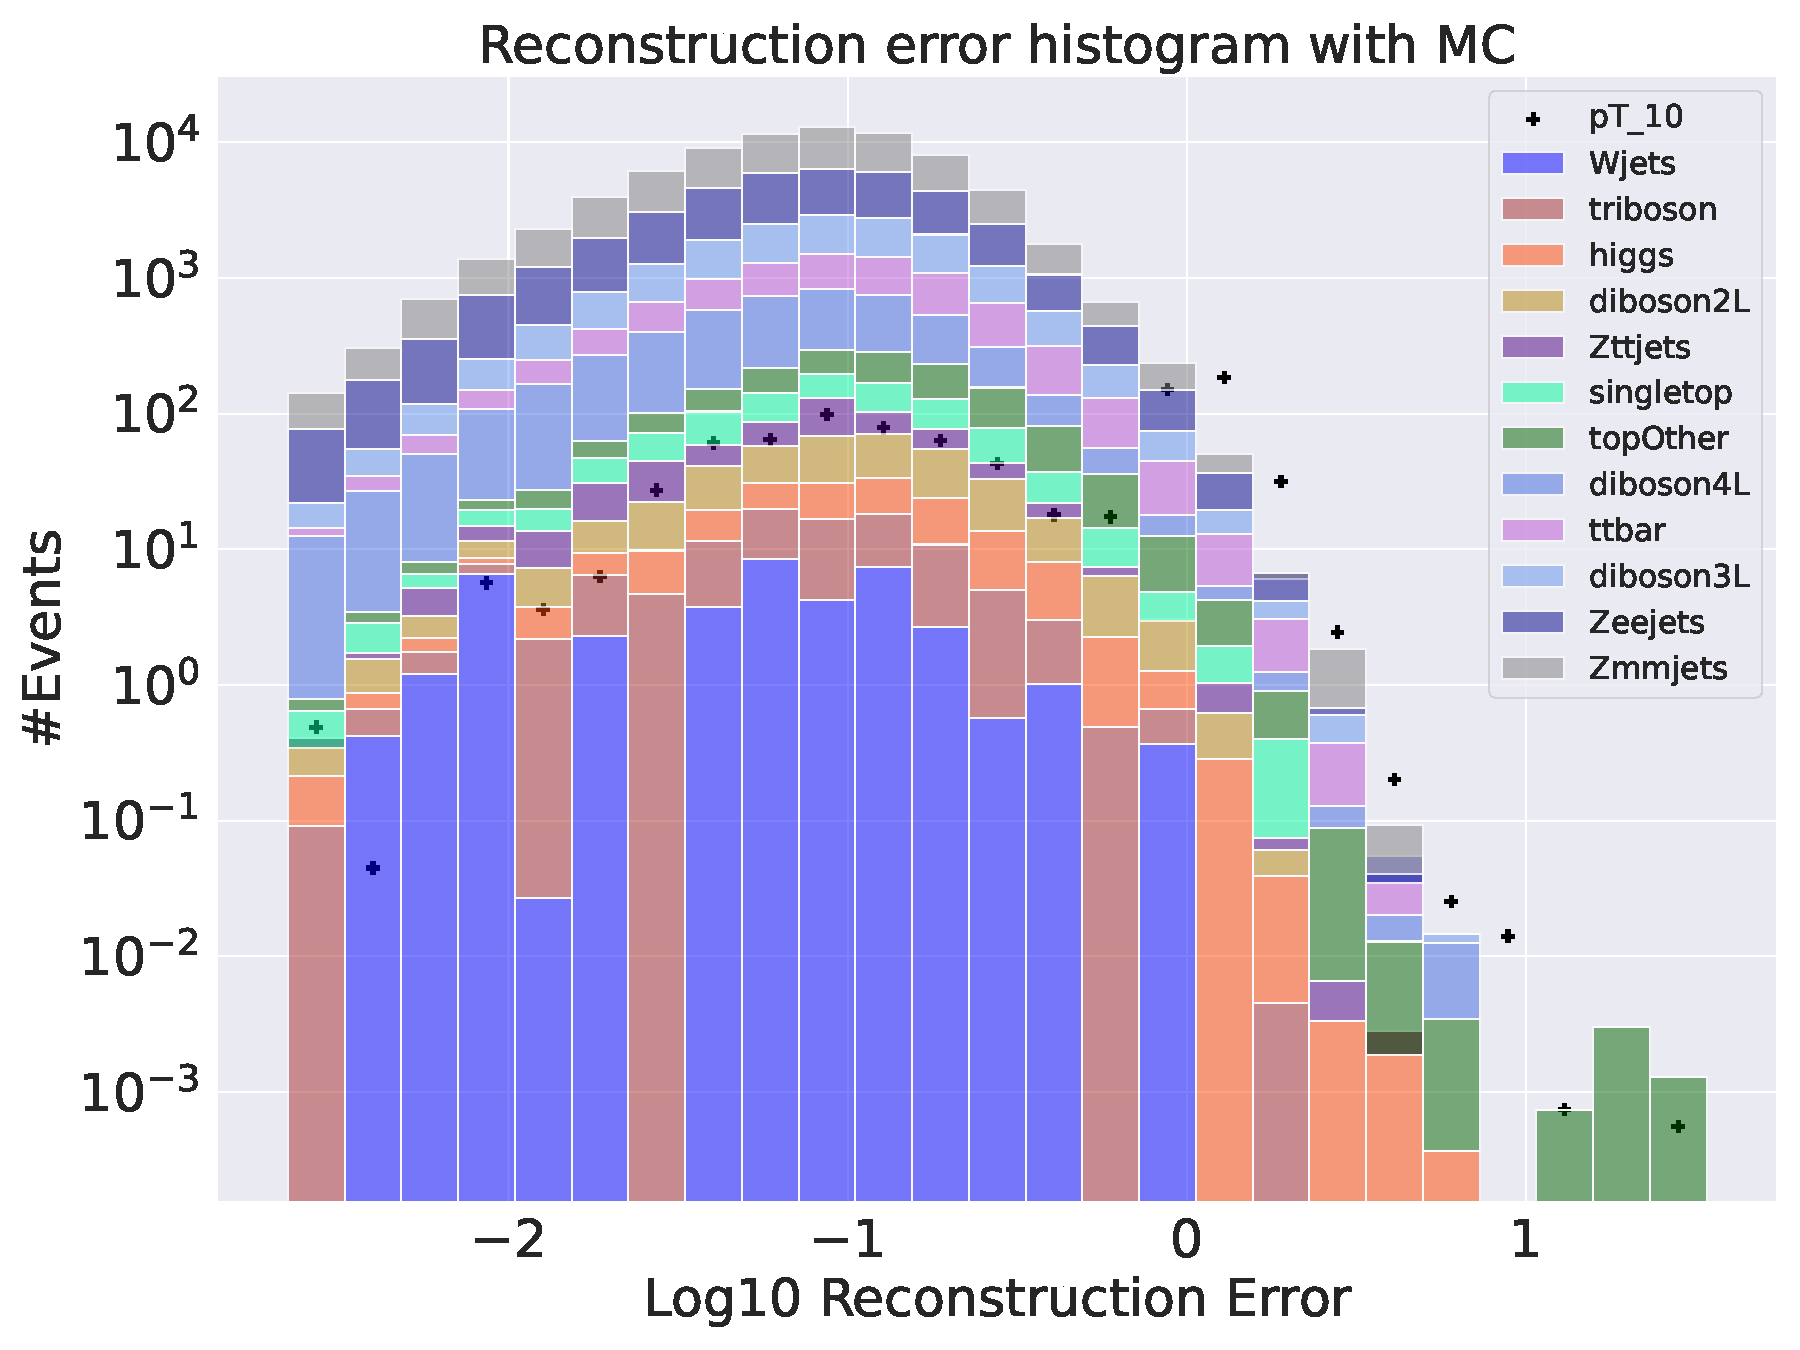
\includegraphics[width=\textwidth]{Figures/VAE_testing/small/b_data_recon_big_rm3_feats_sig_pT_10.pdf}
        \caption{ }
        \label{fig:VAE_small_pt_10}
    \end{subfigure}
    \hfill 
    \begin{subfigure}{.45\textwidth}
        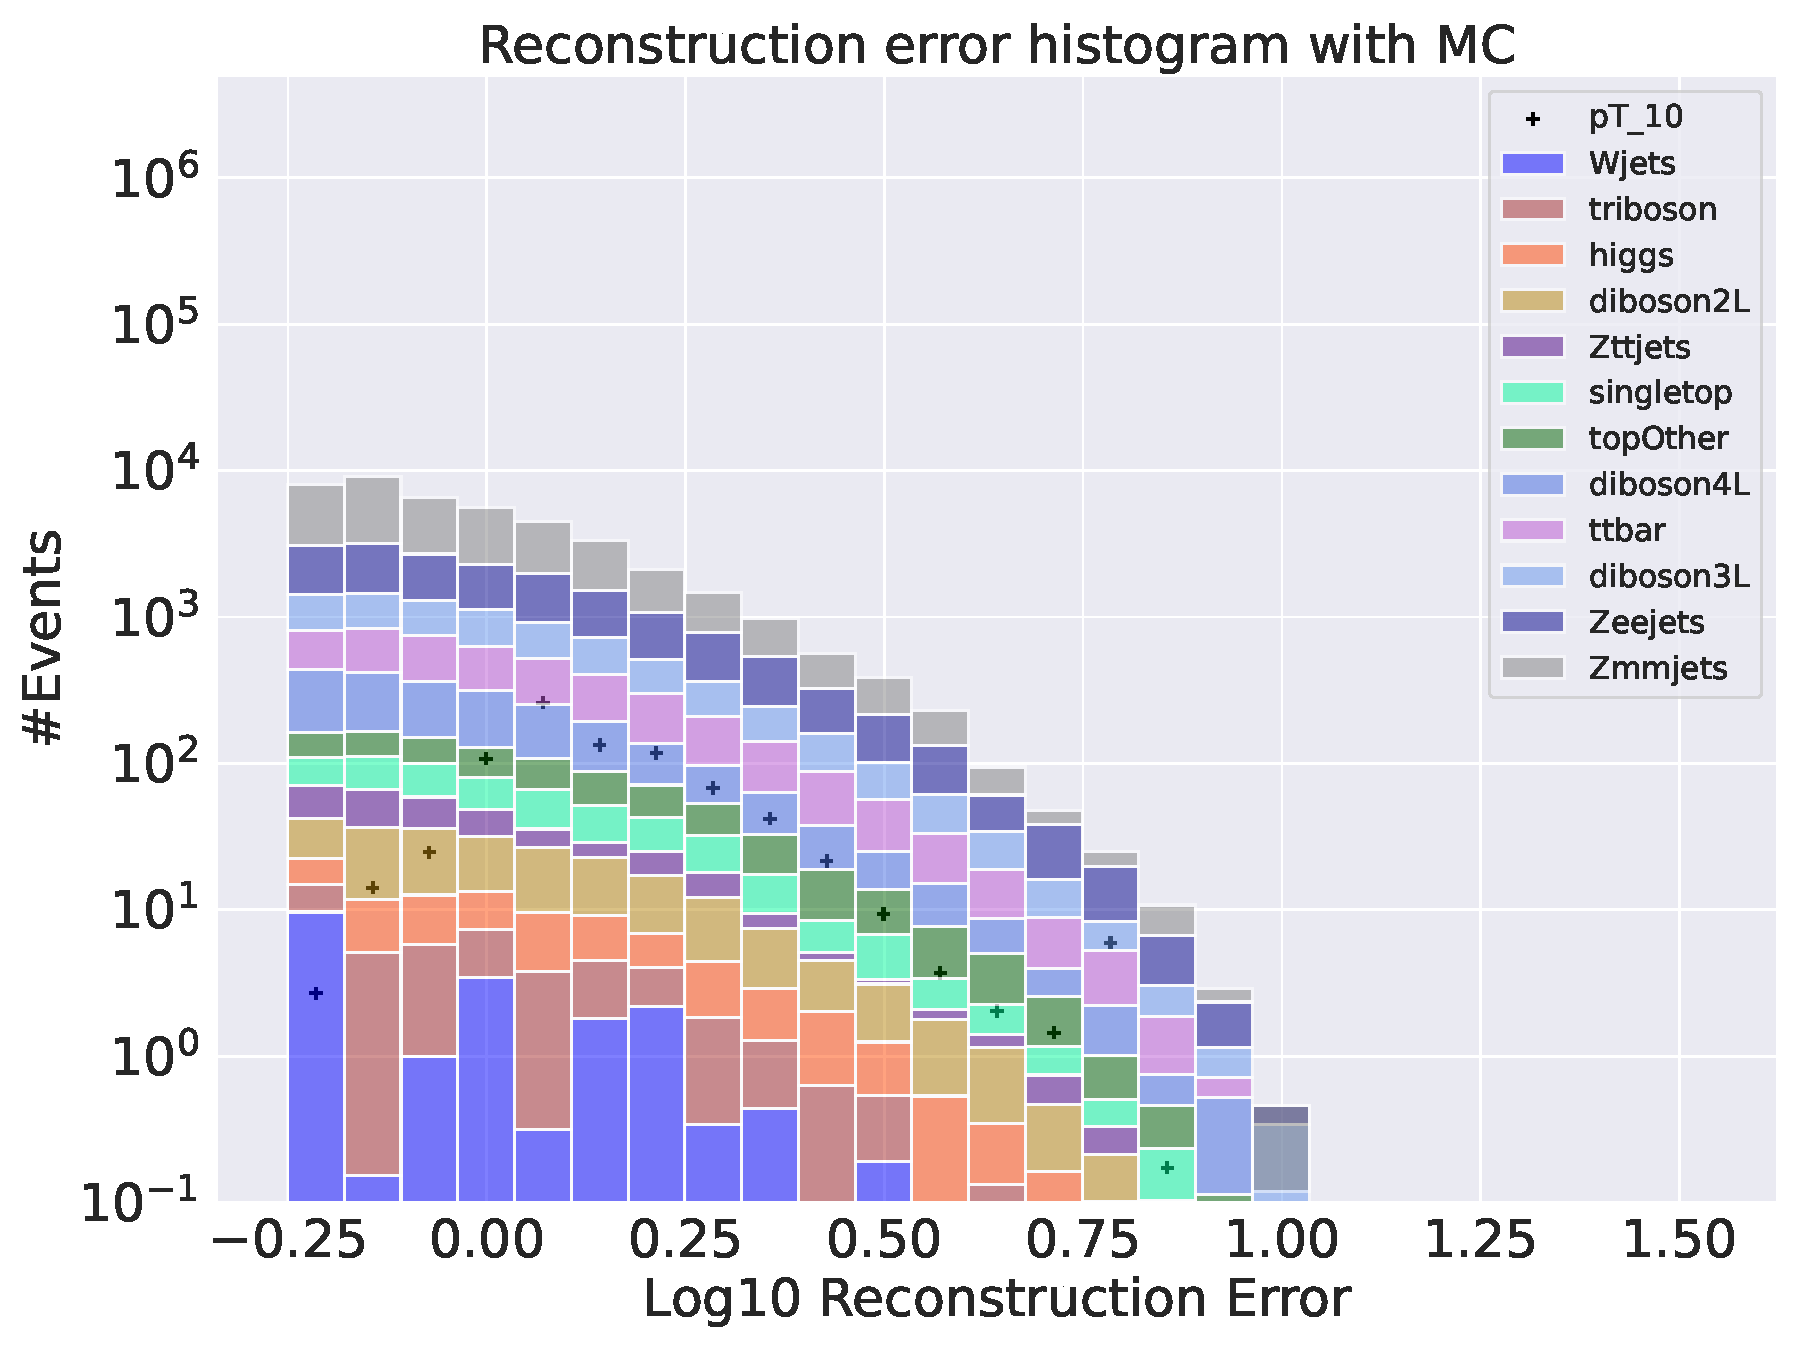
\includegraphics[width=\textwidth]{Figures/VAE_testing/big/b_data_recon_big_rm3_feats_sig_pT_10.pdf}
        \caption{}
        \label{fig:VAE_big_pt_10}
    \end{subfigure}
    \hfill 
    \caption[VAE | Reconstruction error $p_T$ altering of 10]{Reconstruction error on validation SM MC from the small (a) and large (b) variational Autoencoder. The signal is a subsample of the validation 
    set where the transverse momentum of the first electron and the first muon has been increased with a scale of $10$. The change of transverse 
    energy has also been changed according to the scaling of transverse momentum. No significant difference in distributions is found. }
    \label{fig:VAE_big_small_pt_10}
\end{figure}
\hl{Refer to figure names to distringuish between regular and variational in sentence below.}
The first thing to notice here is that, as with the channel removal, the distribution shape of the output from the regular autoencoder compared to the
variational autoencoder is different. The shape from the regular autoencoder is clearly shifted to the left end, with low reconstruction error compared 
to the shape from the variational autoencoder, where the peak of the distribution is around 1. From the $p_T$ altering test we also see here that the 
variational autoencoder falls short to the regular one. It is also interesting to observe here that the high $p_T$ events are picked up as anomalous from both
autoencoders, with both shallow and deep structure. In the regular autoencoder it is arguably even separated distributions. This is also a good sign as it 
indicates that the network has learned which ranges the $p_T$ should be in for the 3 lepton plus missing energy final state. The most extreme case is 
as expected in the case where the $p_T$ is multiplied by 10 \hl{Forklar hvorfor det er forventa}, and the $\delta e_T^{10}$. There is a clear separation in reconstruction error distributions for the
signal and background for the deep regular autoencoder, and a slightly more subtle separation of reconstruction error distributions for the shallow regular autoencoder.
In the variational autoencoder, the separation is not as clear, but the signal is still picked up as anomalous. The peaks are separated, but not to the same degree. 

